\documentclass[11pt,a4paper]{article}

\usepackage[utf8]{inputenc}
\usepackage[T1]{fontenc}
\usepackage[spanish, es-nodecimaldot]{babel}
\addto\captionsspanish{\renewcommand{\tablename}{Tabla}}
\usepackage{geometry}
\geometry{margin=2.5cm}
\usepackage{booktabs}
\usepackage{array}
\usepackage{multirow}
\usepackage{hyperref}
\hypersetup{colorlinks=true, linkcolor=black, urlcolor=blue}
\usepackage{parskip}
\usepackage{listings}
\usepackage{xcolor}
\usepackage{enumitem}
\usepackage{graphicx}
\usepackage{url}
\graphicspath{{diagrams/}}
\usepackage{float}
\usepackage{caption}
\usepackage{rotating}
\usepackage{pdflscape}
\usepackage{colortbl}
\usepackage{amssymb}
\usepackage{inconsolata}

\usepackage{color}

\definecolor{pblue}{rgb}{0.13,0.13,1}
\definecolor{pgreen}{rgb}{0,0.5,0}
\definecolor{pred}{rgb}{0.9,0,0}
\definecolor{pgrey}{rgb}{0.46,0.45,0.48}

\definecolor{lightgray}{gray}{0.92}
\definecolor{codered}{RGB}{180,30,30}
\definecolor{codegreen}{RGB}{0,120,0}
\definecolor{codegray}{RGB}{100,100,100}
\definecolor{warnorange}{RGB}{200,100,0}

\lstset{
  language=Java,
  basicstyle=\ttfamily\footnotesize,
  keywordstyle=\color{pblue},
  commentstyle=\color{codegray}\itshape,
  stringstyle=\color{pred},
  showstringspaces=false,
  showspaces=false,
  showtabs=false,
  breaklines=true,
  breakatwhitespace=false,
  postbreak=\mbox{\textcolor{codegray}{$\hookrightarrow$}\space},
  frame=single,
  framesep=4pt,
  xleftmargin=6pt,
  xrightmargin=6pt,
  aboveskip=6pt,
  belowskip=6pt,
  numbers=left,
  numberstyle=\tiny\color{codegray},
  numbersep=5pt,
  captionpos=b,
  moredelim=[il][\textcolor{pgrey}]{$$},
  moredelim=[is][\textcolor{pgrey}]{\%\%}{\%\%}
}
\renewcommand{\lstlistingname}{Listado}

\newcommand{\code}[1]{\texttt{#1}}
\setlength{\emergencystretch}{3em}  % reduce overfull hboxes en párrafos con código largo
\newcommand{\bad}[1]{\textcolor{codered}{\textbf{#1}}}
\newcommand{\good}[1]{\textcolor{codegreen}{\textbf{#1}}}
\newcommand{\warn}[1]{\textcolor{warnorange}{\textbf{#1}}}

\title{Rediseño de las clases de potenciales\\
       \large Análisis de problemas y opciones de diseño\\[4pt]
       \normalsize \code{org.openmarkov.core} --- paquete \code{model.network.potential}}
\author{Manuel Arias Calleja}
\date{Marzo de 2026}

\begin{document}

\maketitle
\tableofcontents
\newpage

% ===================================================================
\section*{Resumen}

Las clases del paquete \code{potential} de \code{org.openmarkov.core} presentan
problemas de diseño estructurales acumulados a lo largo de varios años de
desarrollo.  El más grave es que \code{TablePotential} ---la clase de la que
depende prácticamente todo el motor de inferencia--- mezcla tres abstracciones
distintas en una sola clase mediante campos opcionales que pueden ser \code{null}.
A esto se añaden métodos abstractos que la mayor parte de las subclases no
pueden implementar, dependencias cíclicas, y un uso extensivo de \emph{downcasts}
en el módulo de inferencia que rompe el polimorfismo y produce fallos en tiempo
de ejecución.

Este documento describía los problemas con detalle, propone cinco opciones
de rediseño de distinto alcance e impacto, y evalúa cada una en términos de
coste de implementación, riesgo, ventajas de diseño e impacto en el rendimiento
(tiempo de cómputo y memoria).

% ===================================================================
\section{Fundamentos teóricos}
\label{sec:fundamentos}

Antes de analizar los problemas concretos del código es conveniente definir los
conceptos de ingeniería del software que se emplean a lo largo del documento.
Esta sección introduce los \emph{principios de diseño} que guían las decisiones
de refactorización, los \emph{antipatrones} que describen los problemas
encontrados, y los \emph{patrones de diseño} aplicados en las soluciones.

% -------------------------------------------------------------------
\subsection{Principios de diseño orientado a objetos}
\label{sec:fund-principios}

Los principios de diseño son reglas generales que, cuando se aplican con
criterio, producen código más fácil de entender, modificar y probar.  No son
recetas infalibles, sino guías que ayudan a tomar decisiones de diseño
razonadas.  A continuación se describen los cuatro principios centrales de
este documento.

\label{sec:fund-srp}
\paragraph{Principio de Responsabilidad Única (SRP)}

El \emph{Single Responsibility Principle} (Principio de Responsabilidad Única)
establece que una clase debe tener una sola razón para cambiar~\cite{martin2003}.
Intuitivamente: si un módulo hace demasiadas cosas a la vez, cualquier cambio
en una de ellas obliga a revisar y probar todas las demás.  Imagina un empleado
encargado a la vez de contabilidad, recursos humanos y soporte técnico: una
auditoría contable, un cambio en las políticas de vacaciones y un fallo en el
servidor afectan al mismo empleado, aunque no tengan nada en común.  Cuando una
clase viola el SRP, sus métodos se entrelazan y las modificaciones en una parte
producen efectos secundarios inesperados en otra.

\label{sec:fund-lsp}
\paragraph{Principio de Sustitución de Liskov (LSP)}

El \emph{Liskov Substitution Principle} (Principio de Sustitución de Liskov)
establece que si una clase $B$ extiende una clase $A$, entonces cualquier
fragmento de código que funcione correctamente con objetos de tipo $A$ debe
seguir funcionando correctamente si se le pasa un objeto de tipo $B$~\cite{liskov1994}.
En términos cotidianos: si en una receta de cocina se dice ``usa un pájaro'',
un pato debería servir.  Pero si la receta dice ``haz volar el pájaro'', un
pingüino ---que es un pájaro--- no sirve, aunque la herencia biológica lo
incluya.  Cuando una subclase no puede cumplir el contrato del padre (porque
devuelve \code{null} o lanza una excepción donde se espera un resultado válido),
el código que usa esa subclase se vuelve frágil e impredecible.

\label{sec:fund-isp}
\paragraph{Principio de Segregación de Interfaces (ISP)}

El \emph{Interface Segregation Principle} (Principio de Segregación de Interfaces)
establece que una clase no debe ser obligada a depender de métodos que no
utiliza.  Cuando se definen interfaces demasiado genéricas, las clases que las
implementan acaban llenando de métodos vacíos o que lanzan excepciones.  Es
preferible tener muchas interfaces pequeñas y específicas que una sola interfaz
grande: así cada clase implementa exactamente las capacidades que tiene, sin
fingir que soporta operaciones que no puede realizar.  Una biblioteca de una
ciudad debería ofrecer servicios de préstamo, consulta y devolución; no debería
verse obligada a ofrecer también reparación de libros o encuadernación solo
porque esos servicios forman parte de un hipotético ``contrato de biblioteca
completa''.

\label{sec:fund-ocp}
\paragraph{Principio Abierto/Cerrado (OCP)}

El \emph{Open/Closed Principle} (Principio Abierto/Cerrado) establece que una
clase debe estar \emph{abierta} para extensión ---se pueden añadir nuevos
comportamientos--- pero \emph{cerrada} para modificación ---no es necesario
cambiar el código existente para añadir esos comportamientos---.  Esto se logra
normalmente mediante herencia o interfaces: en lugar de añadir un nuevo
\code{case} a un \code{switch} existente cada vez que aparece un nuevo tipo,
se crea una nueva subclase o implementación de interfaz.  El código original
no necesita tocarse; el nuevo comportamiento se encapsula en el nuevo tipo.
La ventaja es que el código que ya funciona y ha sido probado permanece intacto,
reduciendo el riesgo de introducir errores al añadir funcionalidad.

% -------------------------------------------------------------------
\subsection{Antipatrones encontrados}
\label{sec:fund-antipatrones}

Un \emph{antipatrón} es un patrón recurrente de diseño que en apariencia
parece razonable pero que en la práctica genera problemas de mantenimiento,
fragilidad o dificultad de comprensión.  Reconocer los antipatrones en el
código propio es el primer paso para corregirlos.

\label{sec:fund-god-class}
\paragraph{God Class (Clase Dios)}

\textbf{Descripción:} Una clase que acumula demasiadas responsabilidades:
lo sabe todo y lo hace todo.  En lugar de delegar en otras clases, concentra
lógica de distintos dominios en una sola unidad.

\textbf{Por qué es dañina:} Viola directamente el SRP.  Cualquier cambio en
cualquiera de sus responsabilidades requiere entender la clase entera, porque
los distintos dominios están entrelazados en los mismos métodos y los mismos
campos.  Las pruebas unitarias son difíciles de escribir porque hay demasiadas
combinaciones posibles de estado.  La God Class se convierte en el cuello de
botella del desarrollo: todo pasa por ella.

\textbf{Solución habitual:} Identificar las distintas responsabilidades que
la clase acumula y extraer cada una a su propia clase.  Esto es exactamente
lo que la refactorización ``Extraer Clase'' (\emph{Extract Class}) persigue.

\label{sec:fund-type-code}
\paragraph{Type Code (Código de Tipo)}

\textbf{Descripción:} Usar un campo numérico o enumerado para hacer que una
clase se comporte de modo diferente según su valor, en lugar de usar subclases
con comportamiento propio.  El resultado es una clase llena de sentencias
\code{switch} o bloques \code{if-else} que inspeccionan el campo para decidir
qué hacer.

\textbf{Por qué es dañino:} Añadir un nuevo ``tipo'' exige rastrear y
modificar \emph{todos} los \code{switch}/\code{if} que miran ese campo,
dispersos por la clase o incluso por el proyecto.  El compilador no avisa de
los casos olvidados.  Cada vez que se añade un valor al enumerado, hay que
analizar manualmente qué bloques de código necesitan actualizarse.

\textbf{Solución habitual:} Reemplazar el campo de tipo por una jerarquía de
subclases (cada subclase representa uno de los tipos) cuyo comportamiento
diferenciado se expresa mediante métodos sobreescritos.  Los patrones de diseño
State y Strategy son formalizaciones de esta solución.

\label{sec:fund-refused-bequest}
\paragraph{Refused Bequest (Legado Rechazado)}

\textbf{Descripción:} Una subclase hereda métodos del padre que no puede o no
quiere implementar, y los deja vacíos o lanzando excepciones.  La subclase
``rechaza la herencia'' que le corresponde.

\textbf{Por qué es dañino:} Viola el LSP: el código que invoca un método sobre
la clase padre puede recibir \code{null} o una excepción donde espera un
resultado válido.  Esto obliga a insertar comprobaciones defensivas en todo el
código que llama a esos métodos, ensuciando el código cliente y desplazando la
responsabilidad de gestionar casos incorrectos fuera de donde debería estar.

\textbf{Solución habitual:} Si una subclase no puede cumplir el contrato del
padre, la relación de herencia es incorrecta.  La solución es retirar la herencia
y usar composición o interfaces que describan solo las capacidades que la clase
verdaderamente posee.

\label{sec:fund-alias-bug}
\paragraph{Aliasing Bug (Error de Alias)}

\textbf{Descripción:} Dos variables apuntan al mismo objeto mutable en memoria
sin que el programador sea consciente de ello.  Modificar el objeto a través de
una variable afecta silenciosamente a la otra, produciendo efectos secundarios
no intencionados.

\textbf{Por qué es dañino:} Produce corrupción de datos difícil de reproducir
y depurar, especialmente en algoritmos que copian y modifican estructuras de
datos.  El fallo se manifiesta lejos del punto donde se introduce el alias, lo
que hace muy difícil encontrar la causa raíz con un depurador.

\textbf{Solución habitual:} Usar \emph{copias defensivas} (\emph{defensive
copy}) al crear o retornar objetos mutables: en lugar de asignar la referencia
al mismo objeto, se crea una nueva instancia con el mismo contenido.  De este
modo, modificar la copia no afecta al original.

% -------------------------------------------------------------------
\subsection{Patrones de diseño aplicados}
\label{sec:fund-patrones}

Un \emph{patrón de diseño} es una solución reutilizable a un problema
frecuente de diseño orientado a objetos~\cite{gamma1995}.  A diferencia de los
antipatrones, los patrones de diseño son soluciones contrastadas.  Este
documento aplica dos patrones.

\label{sec:fund-template-method}
\paragraph{Método Plantilla (Template Method)}

\textbf{Descripción:} La clase base define el esqueleto de un algoritmo
llamando a métodos que las subclases pueden sobreescribir.  La clase base
controla la estructura y el orden de los pasos; las subclases aportan los
detalles específicos de cada paso.  Así, el algoritmo general se escribe
una sola vez en el padre, y solo las partes que varían se delegan a los hijos.

\textbf{Aplicación en este documento:} El método \code{isUncertain()} en la
clase base \code{TablePotential} funciona correctamente para toda la jerarquía
porque llama a \code{getUncertainValues()}, que es un método virtual.  Las
subclases sobreescriben \code{getUncertainValues()} para devolver su array
propio; la clase base no necesita saber qué subclase concreta está en uso.

\label{sec:fund-marker-interface}
\paragraph{Interfaz Marcadora (Marker Interface)}

\textbf{Descripción:} Una interfaz sin métodos que actúa como etiqueta de tipo.
Su presencia en la declaración de una clase comunica al compilador ---y al
lector del código--- que esa clase pertenece a una categoría específica.  El
compilador puede entonces verificar que solo los tipos correctos se usan en
ciertos contextos.

\textbf{Aplicación en este documento:} La interfaz \code{CEUtilityPotential}
marca los potenciales válidos como utilidad en el análisis coste-efectividad.
Solo \code{TablePotential} y \code{GTablePotential} implementan esta interfaz,
garantizando en tiempo de compilación que no lleguen tipos inadecuados a los
algoritmos de fusión del módulo de coste-efectividad.

% ===================================================================
\section{Situación anterior: diagnóstico detallado}

\subsection{Jerarquía de clases}

La jerarquía de \code{Potential} contenía más de treinta subclases que
cubren desde tablas de probabilidad discretas hasta distribuciones gaussianas,
potenciales de función simbólica, árboles de decisión y potenciales de
incertidumbre de modelo.  La clase base abstracta declara ocho métodos abstractos
que todos sus descendientes debían implementar, independientemente de si la
operación tiene sentido para ese tipo de potencial.

Las clases más relevantes para la inferencia son:

\begin{itemize}
  \item \code{TablePotential}: tabla de probabilidades o utilidades sobre variables
        discretas.  Es la clase de trabajo de casi todos los algoritmos.
  \item \code{GTablePotential<E>}: tabla genérica que almacena objetos en lugar
        de \code{double}; usada en el análisis coste-efectividad para almacenar
        objetos \code{Choice}.
  \item \code{UniformPotential}, \code{DeltaPotential}: representaciones compactas
        de distribuciones uniformes y deterministas.
  \item \code{SumPotential}, \code{ProductPotential}: nodos supervalor para
        diagramas de influencia con múltiples funciones de utilidad.
  \item \code{TreeADDPotential}, \code{StrategyTree}: árboles de decisión
        algebráicos y árboles de estrategia de intervención.
\end{itemize}

\subsection{Problema 1: \code{TablePotential} con tres responsabilidades}
\label{sec:prob1}

\code{TablePotential} tiene 1.413~líneas de código.  Su responsabilidad
declarada es almacenar una tabla de valores \code{double} indexada por las
configuraciones de sus variables (antipatrón \emph{God Class},
véase la sección~\ref{sec:fund-god-class}).  Sin embargo, contiene además dos
responsabilidades adicionales mediante campos opcionales:

\begin{lstlisting}[caption={Campos principales de \code{TablePotential}}]
public volatile double[]         values;         // probabilidades/utilidades
public volatile StrategyTree[]   strategyTrees;  // OPCIONAL: intervenciones
public volatile UncertainValue[] uncertainValues;// OPCIONAL: incertidumbre
\end{lstlisting}

El campo \code{strategyTrees} almacena, para cada configuración de la tabla, un
árbol de decisión que codifica las acciones óptimas a ejecutar en las variables
de decisión del problema.  Está presente
únicamente en potenciales de utilidad dentro de la resolución de diagramas de
influencia.  El campo \code{uncertainValues} almacena distribuciones de
incertidumbre sobre cada valor de la tabla para el análisis de sensibilidad
paramétrica.  Ambos campos son \code{null} en la inmensa mayoría de los
potenciales del sistema.

La consecuencia directa es que todos los métodos relevantes de la clase tienen
que manejar tres casos a la vez:

\begin{lstlisting}[caption={Fragmento de \code{tableProject()} con condicionales por campos opcionales}]
boolean hasUncertainTable = (uncertainValues != null);
if (hasUncertainTable) {
    projectedPotential.setUncertainValues(new UncertainValue[length]);
}
// ...
projectedPotential.copyValuesInterventionsAndUncertainValues(
        projectedPosition, this, firstPosition, hasUncertainTable);
// ...
if (strategyTrees != null) {
    resultPotential.strategyTrees = new StrategyTree[resultPotential.values.length];
    for (int i = 0; i < resultPotential.strategyTrees.length; i++) {
        resultPotential.strategyTrees[i] = ...;
    }
}
\end{lstlisting}

Este patrón se repite en \code{reorder()}, \code{deepCopy()}, \code{copy()} y
en los métodos de fusión de \code{TablePotentialMerge}.  La complejidad
efectiva de cada operación sobre potenciales es el triple de la que debería
ser.

Además, el constructor de copia no realiza una copia profunda de los arrays
opcionales:

\begin{lstlisting}[caption={Error de copia superficial en el constructor de copia}]
// Constructor de copia de TablePotential -- los arrays opcionales NO se clonan
uncertainValues = potential.uncertainValues; // alias mutable compartido
strategyTrees   = potential.strategyTrees;   // alias mutable compartido
\end{lstlisting}

Modificar \code{uncertainValues} o \code{strategyTrees} en la copia modifica
también el original, lo que puede causar corrupción silenciosa de datos durante
la inferencia (antipatrón \emph{Aliasing Bug}, sección~\ref{sec:fund-alias-bug}).

\subsection{Problema 2: métodos abstractos que las subclases no pueden implementar}
\label{sec:prob2}

La clase abstracta \code{Potential} declara métodos que muchas subclases son
incapaces de implementar significativamente.  El resultado es una acumulación de
implementaciones déficit que violan el Principio de Sustitución de Liskov
(LSP, sección~\ref{sec:fund-lsp}; antipatrón \emph{Refused Bequest},
sección~\ref{sec:fund-refused-bequest}):

\begin{lstlisting}[caption={Implementaciones forzadas que no tienen sentido para la subclase}]
// UniformPotential -- reorder no implementado
@Override
public Potential reorder(List<Variable> newOrderOfVariables) {
    return null; // TODO Auto-generated method stub
}

// UniformPotential -- project no soportado
@Override
public Potential project(EvidenceCase evidenceCase) {
    throw new NotSupportedOperationException();
}

// UniformPotential -- scalePotential irrelevante (no tiene valores)
@Override
public void scalePotential(double scale) {
    // vacio: no hay nada que escalar
}
\end{lstlisting}

El mismo patrón aparece en \code{DeltaPotential}, \code{SumPotential},
\code{ProductPotential} y otras subclases.  Desde el punto de vista del llamador,
invocar \code{reorder()} sobre cualquier \code{Potential} puede retornar
\code{null}, lo que obliga a insertar comprobaciones defensivas en todo el código
que llama a este método.

La tabla~\ref{tab:metodos-abstractos} resume la situación por método y
subclase.

\begin{table}[H]
\centering
\small
\begin{tabular}{lccccc}
\toprule
\textbf{Método} & \textbf{TablePotential} & \textbf{Uniform} & \textbf{Delta} & \textbf{Sum/Product} & \textbf{ExactDistr} \\
\midrule
\code{tableProject()} & Complejo & Crea tabla & Crea tabla & Delega & Delega \\
\code{project()}      & Delega   & \bad{Excepción} & \bad{Excepción} & \bad{Excepción} & Delega \\
\code{reorder(List)}  & 50 líneas & \bad{null} & \bad{null} & \bad{null} & Delega \\
\code{scalePotential()} & Multiplica & \bad{Vacío} & Multiplica & \bad{Vacío} & Delega \\
\code{isUncertain()}  & Consulta campo & \warn{false} & \warn{false} & \warn{false} & Delega \\
\code{copy()}         & Copia profunda & Copia & Copia & Copia & Copia \\
\bottomrule
\end{tabular}
\caption{Implementación de métodos abstractos por subclase.  \bad{Rojo}: implementación
         incorrecta o ausente.  \warn{Naranja}: trivial/forzada.}
\label{tab:metodos-abstractos}
\end{table}

\subsection{Problema 3: \code{GTablePotential<E>} viola el contrato de su padre}
\label{sec:prob3}

\code{GTablePotential<E>} extiende \code{TablePotential} para almacenar objetos
genéricos (objetos \code{Choice} en el análisis coste-efectividad) en lugar de
valores \code{double}.  Sin embargo, esta relación de herencia es incorrecta:

\begin{lstlisting}[caption={Constructor de \code{GTablePotential} que viola el contrato del padre}]
public GTablePotential(List<Variable> variables, PotentialRole role) {
    super(variables, null); // pasa null como role -- invalida setUniform()
    // ...
    elementTable = new ArrayList<E>(sizeTable);
}
\end{lstlisting}

Al pasar \code{null} como \code{role}, el constructor del padre no puede inicializar
\code{values} correctamente.  El array \code{values} heredado se reserva y se
rellena con ceros pero nunca se usa: \code{GTablePotential} almacena sus datos en
\code{List<E> elementTable}.  Esto supone un desperdicio de memoria (un array de
\code{double} completamente inútil) y hace que todos los métodos heredados que
acceden a \code{values} devuelvan resultados sin sentido.

\subsection{Problema 4: \emph{downcasts} en inferencia}
\label{sec:prob4}

El módulo \code{org.openmarkov.inference} trabaja en la práctica con
\code{TablePotential} directamente, no con \code{Potential}
polimórficamente.  El resultado es un código sembrado de \emph{downcasts}:

\begin{lstlisting}[caption={\emph{Downcasts} desprotegidos en el motor de inferencia}]
// VariableEliminationCore.java
for (Potential potential : probPotentials) {
    probTP.add((TablePotential) potential);   // sin instanceof
}

// VEPropagation.java
posteriorValue = (TablePotential) posteriorValue.reorder(orderedVariables);

// VariableElimination.java
TablePotential utility = new TablePotential(null, PotentialRole.UNSPECIFIED);
\end{lstlisting}

Si en cualquier momento un potencial no es un \code{TablePotential} (porque se usa
una red con \code{UniformPotential}, por ejemplo, y \code{tableProject()} no se
llamó antes), el sistema lanza \code{ClassCastException} en tiempo de ejecución,
lejos del origen del problema y difícil de depurar.

\subsection{Problema 5: dependencia cíclica entre \code{TablePotential} y \code{StrategyTree}}
\label{sec:prob5}

El diseño actual introduce una dependencia cíclica:

\begin{center}
\code{TablePotential} $\longrightarrow$ \code{StrategyTree[]}
\hspace{1em}
\code{StrategyTree} $\longrightarrow$ \code{TreeADDPotential}
\hspace{1em}
\code{TreeADDPotential} $\longrightarrow$ \code{TablePotential}
\end{center}

Este ciclo hace imposible razonar sobre cualquiera de las tres clases de forma
aislada, dificulta las pruebas unitarias y bloquea cualquier intento de
refactorización incremental de la jerarquía.

\subsection{Problema 6: \code{PotentialRole} como sustituto de tipos}
\label{sec:prob6}

El enumerado \code{PotentialRole} (valores: \code{CONDITIONAL\_PROBABILITY},
\code{JOINT\_PROBABILITY}, \code{POLICY}, \code{UTILITY}, \code{LINK\_RESTRICTION},
\code{UNSPECIFIED}) controla el comportamiento de \code{TablePotential} en varios
métodos mediante sentencias \code{switch} y condicionales:

\begin{lstlisting}[caption={\code{PotentialRole} controlando comportamiento en \code{setUniform()}}]
switch (role) {
    case CONDITIONAL_PROBABILITY:
    case POLICY:
        value = 1.0 / variables.get(0).getNumStates();
        break;
    case JOINT_PROBABILITY:
        value = 1.0 / computeTableSize(variables);
        break;
    case LINK_RESTRICTION:
        value = 1.0;
        break;
    default: // UTILITY, UNSPECIFIED
        value = 0.0;
}
\end{lstlisting}

Esto es el antipatrón \emph{type code} (sección~\ref{sec:fund-type-code}): en lugar de subclases con comportamiento
propio, una sola clase se comporta de modo diferente según un campo enum.  Añadir
un nuevo rol exige rastrear y actualizar todos los \code{switch} existentes en la
clase.

% ===================================================================
\section{Opciones de rediseño}

\subsection{Opción 1 --- Extracción mínima de responsabilidades}
\label{sec:op1}

\subsubsection*{Descripción}

Esta opción no modifica la jerarquía de \code{Potential} ni las firmas de los
métodos abstractos.  Su único objetivo es eliminar los dos campos opcionales
de \code{TablePotential} descritos en la sección~\ref{sec:prob1}.

Se crean dos subclases especializadas:

\begin{lstlisting}[caption={Jerarquía resultante de la Opción 1}]
// Clase base sin campos opcionales
class TablePotential extends Potential {
    public volatile double[] values;   // unico campo de datos
    // sin strategyTrees
    // sin uncertainValues
}

// Subclase para potenciales con intervenciones
final class StrategicTablePotential extends TablePotential {
    public StrategyTree[] strategyTrees;

    @Override public boolean hasInterventions() { return true; }
    @Override public Potential deepCopy(ProbNet net) { ... }
    @Override public TablePotential tableProject(...) { ... }
}

// Subclase para potenciales con incertidumbre de modelo
final class UncertainTablePotential extends TablePotential {
    public UncertainValue[] uncertainValues;

    @Override public boolean isUncertain() { return true; }
    @Override public Potential deepCopy(ProbNet net) { ... }
    @Override public TablePotential tableProject(...) { ... }
}
\end{lstlisting}

\code{GTablePotential<E>} deja de extender \code{TablePotential} y pasa a extender
directamente \code{Potential}, eliminando el array \code{values} inútil y el
\code{null} pasado como \code{role}.

Los métodos de \code{Table\-Potential\-Merge}, \code{Table\-Potential\-Maximization} y
\code{Table\-Potential\-Elimination} que actualmente comprueban
\code{if (strategyTrees != null)} o \code{if (uncertainValues != null)} se
simplifican mediante \code{instanceof} o sobrecarga.

\subsubsection*{Lo que no cambia}

\begin{itemize}
  \item Los 28 llamadores de \code{DiscretePotentialOperations} no se tocan.
  \item Los métodos abstractos de \code{Potential} permanecen iguales.
  \item Los \emph{downcasts} en inferencia siguen igual (la inferencia trabaja con
        \code{TablePotential}, que sigue siendo la clase base).
  \item El problema del \code{PotentialRole} como type code no se aborda.
\end{itemize}

\subsubsection*{Ventajas}

\begin{itemize}
  \item \code{TablePotential} pierde $\approx$300~líneas de manejo condicional
        de campos opcionales.
  \item Los métodos \code{reorder()}, \code{deepCopy()} y \code{tableProject()}
        de \code{TablePotential} se simplifican notablemente.
  \item Se elimina el error de copia superficial del constructor de copia: al no
        haber campos opcionales en \code{TablePotential}, no hay alias mutables.
  \item El bug de \code{GTablePotential} (array \code{values} inútil) queda
        resuelto.
  \item Compatible con los tests actuales sin modificación.
\end{itemize}

\subsubsection*{Desventajas}

\begin{itemize}
  \item No resuelve los métodos abstractos forzados (sección~\ref{sec:prob2}).
  \item No elimina los \emph{downcasts} en inferencia (sección~\ref{sec:prob4}).
  \item No rompe la dependencia cíclica (sección~\ref{sec:prob5}).
  \item No aborda el antipatrón \code{PotentialRole} (sección~\ref{sec:prob6}).
\end{itemize}

\subsubsection*{Impacto en rendimiento}

\textbf{Tiempo}: Ligera mejora en todos los métodos de \code{TablePotential} al
eliminar las comprobaciones \code{null} en cada iteración del bucle de offsets
acumulados.  El impacto es pequeño pero consistente: los bucles críticos de
\code{tableProject()} y \code{reorder()} eliminan 2--3 ramas condicionales por
iteración.

\textbf{Memoria}: Reducción moderada.  Los potenciales ordinarios
(\code{TablePotential}) dejan de reservar espacio para dos punteros a arrays
opcionales que en la gran mayoría de los casos son \code{null}.  En el caso
patológico de una red con miles de potenciales, esto puede significar varios
cientos de kilobytes menos en el \emph{heap}.  \code{GTablePotential} deja de
reservar el array \code{values} inútil: ahorro de \code{tableSize * 8 bytes}
por instancia.

\subsubsection*{Esfuerzo estimado}

2--3 semanas.  La mayor parte del trabajo está en extraer \code{StrategicTablePotential}
y \code{UncertainTablePotential} y adaptar \code{TablePotentialMerge} y
\code{TablePotentialMaximization}.

% -------------------------------------------------------------------
\subsection{Opción 2 --- Jerarquía basada en roles}
\label{sec:op2}

\subsubsection*{Descripción}

Esta opción convierte el antipatrón \code{PotentialRole} en una jerarquía de
tipos real.  Cada rol que implica comportamiento distinto se convierte en una
subclase de \code{DiscretePotential}, que a su vez extiende \code{Potential}:

\begin{lstlisting}[caption={Jerarquía resultante de la Opción 2}]
abstract class Potential { ... }

abstract class DiscretePotential extends Potential {
    protected final double[] values;
    protected final int[]    dimensions;
    protected final int[]    offsets;

    // Metodos comunes a todos los potenciales discretos
    public int getPosition(int[] coords) { ... }
    public double[] getValues() { ... }
}

final class ProbabilityPotential extends DiscretePotential {
    // role = CONDITIONAL_PROBABILITY o JOINT_PROBABILITY
    // Sin estrategias, sin incertidumbre
    @Override public ProbabilityPotential tableProject(...) { ... }
    @Override public ProbabilityPotential reorder(...)      { ... }
}

final class UtilityPotential extends DiscretePotential {
    // role = UTILITY
    // Puede tener StrategyTree[]
    private final StrategyTree[] strategyTrees; // no opcional: si existe es StrategicUtility
    @Override public UtilityPotential tableProject(...) { ... }
}

final class PolicyPotential extends DiscretePotential {
    // role = POLICY
    @Override public PolicyPotential tableProject(...) { ... }
}

final class LinkRestrictionPotential extends DiscretePotential {
    // role = LINK_RESTRICTION
}
\end{lstlisting}

Los métodos de operación en \code{DiscretePotentialOperations} y sus clases
delegadas reciben firmas más precisas.  Por ejemplo, \code{multiplyAndMarginalize}
acepta \code{List<ProbabilityPotential>} en lugar de
\code{Collection<TablePotential>}.

El análisis de sensibilidad (\code{UncertainValue}) se modela como un decorador:

\begin{lstlisting}[caption={Decorador para incertidumbre de modelo}]
final class UncertainProbabilityPotential extends ProbabilityPotential {
    private final UncertainValue[] uncertainValues;

    @Override public boolean isUncertain() { return true; }
    // deepCopy() correcto: copia uncertainValues
}
\end{lstlisting}

\subsubsection*{Ventajas}

\begin{itemize}
  \item Elimina completamente el antipatrón \code{PotentialRole} como controlador
        de comportamiento: cada clase tiene su propio \code{setUniform()},
        \code{getInducedFindings()}, etc.
  \item Añadir un nuevo tipo de potencial discreto (p.~ej.\ \code{RewardPotential}
        para MDPs) es añadir una subclase sin tocar las existentes.
  \item Las firmas de las operaciones de inferencia son más precisas y
        los \emph{downcasts} desaparecen en la mayoría de los puntos de llamada.
  \item La dependencia cíclica \code{TablePotential} $\leftrightarrow$
        \code{StrategyTree} queda resuelta: \code{StrategyTree} se asocia solo
        con \code{UtilityPotential}.
\end{itemize}

\subsubsection*{Desventajas}

\begin{itemize}
  \item La frontera entre \code{ProbabilityPotential} y \code{UtilityPotential} es
        difusa en ciertos algoritmos: \code{multiplyAndMarginalize} multiplica una
        probabilidad por una utilidad y produce un resultado híbrido cuyo tipo no
        encaja limpiamente en ninguna de las dos subclases.
  \item Requiere actualizar las firmas de métodos en los llamadores del módulo
        \code{inference}, lo que puede propagar cambios a todos los algoritmos.
  \item Los métodos abstractos forzados (sección~\ref{sec:prob2}) no se
        resuelven en las subclases de \code{Potential} que no son discretas
        (\code{UniformPotential}, \code{DeltaPotential}, etc.).
\end{itemize}

\subsubsection*{Impacto en rendimiento}

\textbf{Tiempo}: Neutro o ligera mejora.  El despacho de métodos virtuales no
cambia en profundidad respecto a la situación actual.  La eliminación de los
\code{switch} sobre \code{PotentialRole} en métodos llamados frecuentemente
(\code{setUniform()}, \code{getInducedFindings()}) supone un ahorro de unos pocos
nanosegundos por llamada, irrelevante en la mayoría de los casos.

\textbf{Memoria}: Reducción moderada.  La eliminación de campos opcionales tiene
el mismo efecto que en la Opción~1.  Las subclases adicionales en la jerarquía
no implican coste de memoria por instancia: solo el coste fijo de la clase en el
\emph{metaspace} de la JVM, que es despreciable.

\subsubsection*{Esfuerzo estimado}

2--3~meses.  El reto mayor es la propagación de cambios al módulo
\code{inference} y a los formatos de E/S.

% -------------------------------------------------------------------
\subsection{Opción 3 --- Composición mediante interfaces}
\label{sec:op3}

\subsubsection*{Descripción}

En lugar de usar herencia para modelar capacidades, esta opción define
\emph{interfaces de capacidad}\footnote{Una \emph{interfaz de capacidad} es una
interfaz Java cuya implementación indica que la clase soporta una operación
específica.  A diferencia de la herencia, una clase puede declarar exactamente
las capacidades que posee sin heredar métodos que no puede implementar.
Este enfoque aplica el Principio de Segregación de Interfaces (ISP,
sección~\ref{sec:fund-isp}).} que las clases implementan según lo que realmente
soportan:

\begin{lstlisting}[caption={Interfaces de capacidad}]
/** Cualquier potencial que puede proyectarse a una tabla discreta. */
interface Projectable {
    TablePotential tableProject(EvidenceCase ev, InferenceOptions opts)
            throws NonProjectablePotentialException;
}

/** Potencial cuyos valores pueden reordenarse segun un nuevo orden de variables. */
interface Reorderable {
    Potential reorder(List<Variable> newOrderOfVariables);
}

/** Potencial que puede escalarse por un factor escalar. */
interface Scalable {
    void scale(double factor);
}

/** Potencial con distribucion de incertidumbre sobre sus valores. */
interface UncertaintyCarrier {
    UncertainValue[] getUncertainValues();
    boolean isUncertain();
}

/** Potencial que lleva arboles de estrategia de intervencion. */
interface StrategyCarrier {
    StrategyTree[] getStrategies();
    boolean hasInterventions();
}
\end{lstlisting}

Las clases implementan solo las interfaces que tienen sentido para ellas:

\begin{lstlisting}[caption={Implementación de interfaces por clase}]
// Clase base simple -- solo capacidad de proyeccion
class TablePotential extends Potential
        implements Projectable, Reorderable, Scalable { ... }

// Con incertidumbre -- a~nade UncertaintyCarrier
class UncertainTablePotential extends TablePotential
        implements UncertaintyCarrier { ... }

// Con estrategias -- a~nade StrategyCarrier
class StrategicTablePotential extends TablePotential
        implements StrategyCarrier { ... }

// Potencial uniforme -- solo proyectable, no reordenable
class UniformPotential extends Potential implements Projectable { ... }

// Potencial delta -- proyectable y escalable
class DeltaPotential extends Potential implements Projectable, Scalable { ... }
\end{lstlisting}

El código de inferencia declara los tipos que necesita en función de las
interfaces:

\begin{lstlisting}[caption={Uso de interfaces en el motor de inferencia}]
// En lugar de: List<TablePotential> probPotentials = ...
List<Projectable> projectable = network.getPotentials().stream()
        .filter(p -> p instanceof Projectable)
        .map(p -> (Projectable) p)
        .collect(toList());

// En lugar de: TablePotential tp = (TablePotential) potential;
if (potential instanceof Reorderable reorderable) {
    Potential reordered = reorderable.reorder(newOrder); // Java 16+
}
\end{lstlisting}

Esta opción también permite combinar capacidades mediante composición:

\begin{lstlisting}[caption={Clase que combina múltiples capacidades}]
class FullCapabilityPotential extends TablePotential
        implements UncertaintyCarrier, StrategyCarrier {
    private final UncertainValue[] uncertainValues;
    private final StrategyTree[]   strategyTrees;
    // ...
}
\end{lstlisting}

\subsubsection*{Ventajas}

\begin{itemize}
  \item Elimina completamente los métodos abstractos forzados: \code{UniformPotential}
        no necesita declarar \code{reorder()} ni \code{scalePotential()} porque no
        implementa \code{Reorderable} ni \code{Scalable}.
  \item Los \emph{downcasts} en inferencia desaparecen: el código pide la
        capacidad que necesita mediante la interfaz apropiada.
  \item Es la opción más extensible: añadir un nuevo tipo de potencial
        equivale a decidir qué interfaces implementa, sin modificar nada más.
  \item Compatible con Java~21 (\emph{pattern matching} para \code{instanceof}
        simplifica el código de consumo).
\end{itemize}

\subsubsection*{Desventajas}

\begin{itemize}
  \item Requiere revisar \emph{todo} el módulo \code{inference} para sustituir
        los usos directos de \code{TablePotential} por interfaces.
  \item El impacto se extiende a los módulos \code{gui}, \code{io} y \code{learning},
        que también crean y manipulan potenciales.
  \item La abstracción de interfaces añade una capa de indirección que
        algunos desarrolladores pueden encontrar menos legible que la herencia
        directa.
  \item Las operaciones de aritmética (\code{DiscretePotentialOperations}) deben
        ser revisadas para aceptar interfaces en lugar de clases concretas, lo
        que puede requerir sobrecargas adicionales.
\end{itemize}

\subsubsection*{Impacto en rendimiento}

\textbf{Tiempo}: Impacto negativo pequeño.  El despacho de métodos de interfaz
(\emph{invokeinterface}) es marginalmente más costoso que el despacho de métodos
virtuales (\emph{invokevirtual}) en la JVM: típicamente 1--3~ns por llamada en JVMs
modernas con JIT.  Los bucles críticos de inferencia realizan millones de llamadas
a \code{tableProject()} y a operaciones de tabla; en entornos de producción, este
coste puede acumularse hasta un 2--5\% de ralentización en benchmarks de alta
precisión, aunque en la práctica la JVM puede eliminarlo mediante
devirtualización agresiva.

\textbf{Memoria}: Similar a la Opción~1.  La eliminación de campos opcionales
en \code{TablePotential} tiene el mismo efecto positivo.  Las interfaces en sí
no añaden coste de memoria por instancia.

\subsubsection*{Esfuerzo estimado}

3--4~meses con riesgo de compilación en cascada en módulos dependientes.

% -------------------------------------------------------------------
\subsection{Opción 4 --- Patrón Visitor para separar operaciones de datos}
\label{sec:op4}

\subsubsection*{Descripción}

Esta opción es la más radical: las clases \code{Potential} se convierten en
contenedores de datos puros, y todas las operaciones (proyección, reordenamiento,
escalado, copia profunda) se mueven a clases \emph{Visitor} externas.

\begin{lstlisting}[caption={Jerarquía de datos y visitantes}]
// Datos puros -- sin logica de operacion
abstract class Potential {
    protected final List<Variable> variables;
    abstract <R> R accept(PotentialVisitor<R> visitor);
}

final class TablePotential extends Potential {
    final double[] values;
    @Override public <R> R accept(PotentialVisitor<R> v) { return v.visit(this); }
}

final class UniformPotential extends Potential {
    @Override public <R> R accept(PotentialVisitor<R> v) { return v.visit(this); }
}

// Operaciones -- separadas de los datos
interface PotentialVisitor<R> {
    R visit(TablePotential tp);
    R visit(UniformPotential up);
    R visit(DeltaPotential dp);
    R visit(FunctionPotential fp);
    // un metodo por tipo concreto de Potential
}

// Ejemplo de visitante concreto
class ProjectionVisitor implements PotentialVisitor<TablePotential> {
    private final EvidenceCase evidence;
    private final InferenceOptions opts;

    @Override public TablePotential visit(TablePotential tp) {
        // logica de proyeccion sobre tabla
    }
    @Override public TablePotential visit(UniformPotential up) {
        // proyecta uniforme en una tabla discreta
    }
    @Override public TablePotential visit(DeltaPotential dp) {
        // proyecta delta en una tabla discreta
    }
    // ...
}

// Otros visitantes
class ReorderVisitor   implements PotentialVisitor<Potential>     { ... }
class ScaleVisitor     implements PotentialVisitor<Void>          { ... }
class DeepCopyVisitor  implements PotentialVisitor<Potential>     { ... }
\end{lstlisting}

El código de llamada pasa de:

\begin{lstlisting}
TablePotential projected = potential.tableProject(evidenceCase, options);
\end{lstlisting}

\noindent a:

\begin{lstlisting}
TablePotential projected = potential.accept(new ProjectionVisitor(evidenceCase, options));
\end{lstlisting}

\subsubsection*{Ventajas}

\begin{itemize}
  \item Separación perfecta entre datos y operaciones: las clases \code{Potential}
        no conocen nada de la lógica de operación.
  \item Añadir una nueva operación (p.~ej.\ serializar a formato binario o
        evaluar en GPU) equivale a implementar un nuevo \code{Visitor} sin tocar
        ninguna clase de datos existente.
  \item El compilador garantiza que cada \code{Visitor} maneja todos los tipos de
        potencial: si se añade un nuevo tipo concreto, todos los visitantes
        existentes dejan de compilar hasta que se añade el método correspondiente.
  \item Elimina completamente los métodos abstractos forzados y los
        \emph{downcasts}.
  \item La dependencia cíclica desaparece: los visitantes de \code{StrategyTree}
        y los de \code{TablePotential} son independientes.
\end{itemize}

\subsubsection*{Desventajas}

\begin{itemize}
  \item Añadir un nuevo tipo de \code{Potential} exige actualizar \emph{todos}
        los visitantes existentes.  Con una jerarquía de 30+ tipos y varios
        visitantes, esto puede ser una carga de mantenimiento elevada.
  \item El patrón \code{Visitor} en Java es verboso: requiere una interfaz con
        tantos métodos como tipos concretos, y cada clase concreta implementa
        \code{accept()}.
  \item El cambio afecta a la API pública de \code{Potential}: eliminar
        \code{tableProject()} de la clase base es un cambio incompatible hacia
        atrás que propaga a todos los módulos dependientes.
  \item La indirección añadida puede dificultar la lectura del flujo de código
        para desarrolladores no familiarizados con el patrón.
\end{itemize}

\subsubsection*{Impacto en rendimiento}

\textbf{Tiempo}: Impacto negativo moderado.  Cada operación pasa por una doble
indirección: \code{accept()} despacha a la implementación concreta de
\code{Potential}, que a su vez despacha al método correspondiente del visitante.
En la JVM moderna, el JIT puede eliminar la mayor parte de esta indirección si
los tipos son monomorfos en los puntos de llamada calientes, pero en código de
inferencia ---donde se procesan potenciales de tipos distintos--- el JIT no puede
hacer esta optimización y el coste de indirección puede ser de
5--10\% en tiempo de ejecución en benchmarks intensivos.

\textbf{Memoria}: Cada invocación de una operación crea un objeto \code{Visitor}
(aunque podría reutilizarse mediante un pool).  En bucles de inferencia que
invocan millones de proyecciones, esto supone presión adicional sobre el
\emph{garbage collector}: millones de objetos pequeños de vida muy corta que el
GC debe recolectar.  El impacto depende de la política del GC (G1GC, ZGC) pero
puede aumentar las pausas en un 10--20\% con la configuración por defecto.

\subsubsection*{Esfuerzo estimado}

4--6~meses con alto riesgo de regresiones.  Es la opción más ambiciosa.

% -------------------------------------------------------------------
\subsection{Opción 5 --- Potenciales inmutables con \emph{builder}}
\label{sec:op5}

\subsubsection*{Descripción}

Esta opción mantiene la jerarquía de clases actual pero convierte las instancias
de \code{TablePotential} en objetos inmutables (\emph{value objects}).  Las
operaciones que actualmente mutan los valores (\code{normalize()}, la escritura
directa en \code{potential.values}) devuelven nuevas instancias.  La construcción
se realiza exclusivamente a través de un \emph{builder}:

\begin{lstlisting}[caption={Builder para \code{TablePotential} inmutable}]
final class TablePotential {
    private final List<Variable> variables;
    private final double[]       values;       // copia defensiva en constructor
    private final PotentialRole  role;
    // sin strategyTrees, sin uncertainValues (extraidos a subclases)

    private TablePotential(Builder b) {
        this.variables = List.copyOf(b.variables);
        this.values    = b.values.clone();     // siempre copia defensiva
        this.role      = b.role;
    }

    public static Builder builder(List<Variable> vars, PotentialRole role) {
        return new Builder(vars, role);
    }

    public double[] getValues() { return values.clone(); } // copia defensiva

    public static class Builder {
        private double[]         values;
        private List<Variable>   variables;
        private PotentialRole    role;

        public Builder withValues(double[] v)    { this.values = v.clone(); return this; }
        public TablePotential build()            { return new TablePotential(this); }
    }
}
\end{lstlisting}

Los métodos que actualmente mutan la tabla (por ejemplo, \code{normalize} in-place)
se convierten en métodos que retornan una nueva instancia:

\begin{lstlisting}[caption={Normalización devuelve nueva instancia en lugar de mutar}]
// Antes (mutable):
TablePotential normalized = DiscretePotentialOperations.normalize(potential);
// normalize() modifica potential.values en sitio

// Despues (inmutable):
TablePotential normalized = potential.normalize();
// potential no se modifica; normalized es una nueva instancia
\end{lstlisting}

Esta opción resuelve directamente el bug del constructor de copia (sección
\ref{sec:prob1}): si los objetos son inmutables, no hay alias problemáticos.
Los arrays \code{volatile} dejan de ser necesarios en el caso \emph{single-thread}
(aunque se mantienen en la variante concurrente).

\subsubsection*{Ventajas}

\begin{itemize}
  \item Elimina definitivamente los problemas de aliasing en el constructor de
        copia y en las copias profundas.
  \item \emph{Thread-safety} por diseño: los objetos inmutables pueden compartirse
        entre hilos sin sincronización.  Esto es relevante dado que el paquete
        \code{operation/concurrent/} ya contiene versiones concurrentes de las
        operaciones de multiplicación.
  \item El \emph{builder} hace explícitos los campos opcionales (intervenciones,
        incertidumbre) sin necesidad de subclases adicionales.
  \item El razonamiento local es más fácil: un potencial no cambia una vez
        creado.
\end{itemize}

\subsubsection*{Desventajas}

\begin{itemize}
  \item Varios algoritmos de inferencia mutan \code{potential.values} directamente
        por eficiencia, usando el acceso público al array.  Convertir estos
        accesos a un patrón de copia-en-escritura requiere una refactorización
        significativa.
  \item Las operaciones que crean muchas tablas intermedias (eliminación de
        variables, propagación) generan más objetos de vida corta, aumentando
        la presión sobre el \emph{garbage collector}.
  \item La copia defensiva en \code{getValues()} puede ser un cuello de botella en
        código que accede frecuentemente a los valores: el código actual accede
        a \code{potential.values[i]} directamente en bucles críticos.
  \item No resuelve los métodos abstractos forzados ni los \emph{downcasts} en
        inferencia.
\end{itemize}

\subsubsection*{Impacto en rendimiento}

\textbf{Tiempo}: Impacto negativo potencialmente alto.  La normalización in-place
de potenciales durante la propagación de evidencia es una operación muy
frecuente; convertirla en copia implica reservar y copiar un array de
\code{double[tableSize]} en cada llamada.  Para redes con variables de muchos
estados, \code{tableSize} puede ser de miles a millones de entradas.  En
benchmarks de eliminación de variables con redes densas, este cambio puede
suponer una ralentización del 15--30\%.

\textbf{Memoria}: Impacto negativo significativo.  En un ciclo de propagación
completo sobre una red de tamaño mediano, el número de tablas intermedias puede
ser del orden de cientos; en el modelo mutable cada tabla se reutiliza o se modifica
in-place, mientras que en el modelo inmutable cada operación genera una nueva
instancia.  El uso máximo de memoria (el \emph{heap} en el momento de mayor
actividad) puede aumentar entre un 50\% y un 200\% según la tamaño de la red
y el algoritmo.  El GC necesita más ciclos para limpiar los objetos intermedios.

\subsubsection*{Esfuerzo estimado}

2--3~meses, pero con atención especial a los \emph{hotspots} de rendimiento.

% ===================================================================
\section{Comparativa de opciones}

La tabla~\ref{tab:comparativa} resume las cinco opciones según los criterios
más relevantes.

\begin{landscape}
\begin{table}[p]
\centering
\small
\setlength{\tabcolsep}{5pt}
\begin{tabular}{lp{2.8cm}p{2.8cm}p{2.8cm}p{2.8cm}p{2.8cm}}
\toprule
\textbf{Criterio}
  & \textbf{Op.\,1} \newline Extracción mín.
  & \textbf{Op.\,2} \newline Roles $\to$ tipos
  & \textbf{Op.\,3} \newline Interfaces
  & \textbf{Op.\,4} \newline Visitor
  & \textbf{Op.\,5} \newline Inmutabilidad \\
\midrule
\rowcolor{lightgray}
Esfuerzo estimado
  & 2--3 semanas
  & 2--3 meses
  & 3--4 meses
  & 4--6 meses
  & 2--3 meses \\

Riesgo de regresión
  & Bajo
  & Medio
  & Medio-alto
  & Alto
  & Medio \\

\rowcolor{lightgray}
Elimina campos opcionales
  & \good{Sí}
  & \good{Sí}
  & \good{Sí}
  & \good{Sí}
  & Parcialmente \\

Métodos forzados
  & \bad{No}
  & Parcialmente
  & \good{Sí}
  & \good{Sí}
  & \bad{No} \\

\rowcolor{lightgray}
Elimina \emph{downcasts}
  & \bad{No}
  & Parcialmente
  & \good{Sí}
  & \good{Sí}
  & \bad{No} \\

Rompe dependencia cíclica
  & \bad{No}
  & \good{Sí}
  & \good{Sí}
  & \good{Sí}
  & \bad{No} \\

\rowcolor{lightgray}
Compatibilidad con tests actuales
  & Total
  & Parcial
  & Parcial
  & Ninguna
  & Parcial \\

Impacto en tiempo (inferencia)
  & \good{Ligera mejora} \newline (\textminus2--5 ramas/it.)
  & \good{Neutro / leve mejora}
  & \warn{Leve penalización} \newline (+1--3\,ns/llamada)
  & \warn{Penalización mod.} \newline (+5--10\% en benchmarks)
  & \bad{Penalización alta} \newline (+15--30\% en redes densas) \\

\rowcolor{lightgray}
Impacto en memoria
  & \good{Reducción moderada} \newline (campos null eliminados)
  & \good{Reducción moderada} \newline (igual que Op.\,1)
  & \good{Reducción moderada} \newline (igual que Op.\,1)
  & \warn{Pequeño aumento} \newline (objetos Visitor)
  & \bad{Aumento significativo} \newline (+50--200\% tablas interm.) \\

\bottomrule
\end{tabular}
\caption{Comparativa de las cinco opciones de rediseño.  \good{Verde}: aspecto
         positivo.  \warn{Naranja}: aspecto neutro o moderadamente negativo.
         \bad{Rojo}: aspecto negativo.}
\label{tab:comparativa}
\end{table}
\end{landscape}

% ===================================================================
\section{Valoración y recomendación}

\subsection{Si el objetivo es la estabilidad a corto plazo}

La \textbf{Opción~1} ofrece el mayor beneficio por el menor coste y riesgo.
Resuelve el problema más grave (los campos opcionales y el bug de la copia
superficial) sin necesidad de tocar el módulo de inferencia ni los tests
actuales.  Puede completarse en 2--3~semanas y sirve de base para refactorizaciones
más profundas.

\subsection{Si hay apetito para un rediseño sustancial}

La \textbf{Opción~3} (interfaces) es la que mejor equilibra completitud del
diseño, extensibilidad y viabilidad práctica.  Resuelve todos los problemas
estructurales identificados ---métodos forzados, \emph{downcasts}, campos
opcionales, dependencia cíclica--- sin el coste del patrón Visitor.  La
penalización de rendimiento por despacho de interfaces es real pero pequeña y
la JVM moderna la mitiga en la mayoría de los puntos de llamada calientes.

La \textbf{Opción~2} es una alternativa válida si se prefiere una jerarquía de
herencia a las interfaces, pero la frontera difusa entre \code{ProbabilityPotential}
y \code{UtilityPotential} en las operaciones de multiplicación hace que su diseño
sea más delicado.

\subsection{Lo que se desaconseja}

La \textbf{Opción~5} (inmutabilidad) introduce costes de rendimiento y memoria
que pueden ser inaceptables en redes densas, precisamente los casos en que
OpenMarkov se usa con más frecuencia.  Solo tiene sentido si el rendimiento
en esos escenarios no es crítico o si se adopta junto con una estrategia de
copia diferida (\emph{copy-on-write}).

La \textbf{Opción~4} (Visitor) es elegante teóricamente pero su coste de
mantenimiento ---actualizar todos los visitantes cada vez que se añade un nuevo
tipo de potencial--- puede superar sus ventajas en un proyecto con una jerarquía
de 30+ subclases activamente extendida.

\subsection{Enfoque incremental recomendado}

Independientemente de cuál sea la opción elegida para el largo plazo, se
recomienda el siguiente orden de pasos para minimizar el riesgo:

\begin{enumerate}
  \item \textbf{Aplicar la Opción~1} como primera fase: extraer
        \code{StrategicTablePotential} y \code{UncertainTablePotential}, corregir
        \code{GTablePotential}.  Verificar con los 337 tests del módulo
        \code{core} y los 13 del módulo \code{inference}.
  \item \textbf{Elegir la opción de largo plazo} (2 o 3) y diseñar la migración
        por fases, comenzando por las clases de mayor impacto
        (\code{ProbabilityPotential} / \code{Projectable}).
  \item \textbf{Migrar el módulo de inferencia} como última fase, una vez que
        la jerarquía de potenciales esté estabilizada.
\end{enumerate}

% ===================================================================
% ===================================================================
\newpage
\part{Rediseño 1: Implementación de la Opción 1}
\label{part:rediseno1}

% ===================================================================
\section{Resumen de la implementación}
\label{sec:resumen-impl}

Este capítulo documenta la implementación completa de la Opción~1 descrita
en la sección~\ref{sec:op1}.  El trabajo se realizó en cinco fases incrementales
(de las cuales cuatro están completadas) sobre el módulo
\code{org.openmarkov.core}, sin modificar ningún otro módulo.

El resultado principal es la separación de las tres responsabilidades de
\code{TablePotential} en una jerarquía de clases donde cada subclase encapsula
exactamente un aspecto opcional:

\begin{itemize}
  \item \code{TablePotential} $\to$ solo \code{values[]}: valores numéricos de la
        tabla.
  \item \code{StrategicTablePotential} $\to$ añade \code{strategyTrees[]}: árboles
        de estrategia de intervención para resolución de diagramas de influencia.
  \item \code{UncertainTablePotential} $\to$ añade \code{uncertainValues[]}: distribuciones
        de incertidumbre para análisis de sensibilidad paramétrica.
\end{itemize}

Adicionalmente, la lógica de indexación (dimensiones, offsets, tamaño de tabla)
se extrajo a una nueva clase abstracta \code{AbstractIndexedPotential}, creando un
punto de anclaje para la futura cambio de superclase de \code{GTablePotential}.

\noindent\textbf{Estado tras la implementación:}
\begin{itemize}
  \item 337 tests pasan, 0 fallos.
  \item Se eliminaron $\approx$300 líneas de lógica condicional triple en
        \code{TablePotential}.
  \item El bug de copia superficial del constructor de copia queda eliminado.
  \item 3 clases nuevas creadas, 12 ficheros modificados.
\end{itemize}

% ===================================================================
\section{Fundamentos teóricos del rediseño}
\label{sec:fundamentos-impl}

Los principios de diseño orientado a objetos y los patrones aplicados en este
rediseño se describen con detalle en la sección~\ref{sec:fundamentos}.  Esta
sección aplica esos conceptos al caso concreto de \code{TablePotential} y
explica los mecanismos específicos de Java empleados en la implementación.

\subsection{SRP aplicado: responsabilidades de \texttt{TablePotential}}

El \emph{Single Responsibility Principle}~\cite{martin2003}
(véase la sección~\ref{sec:fund-srp}) exige que cada clase tenga una única
razón para cambiar.  En el diseño anterior,
\code{TablePotential} tenía \textbf{tres} razones para cambiar:

\begin{enumerate}
  \item Cambios en cómo se almacenan o indexan los valores de probabilidad/utilidad.
  \item Cambios en cómo se representan y propagan las intervenciones
        (\code{StrategyTree}).
  \item Cambios en cómo se modela la incertidumbre paramétrica
        (\code{UncertainValue}).
\end{enumerate}

La consecuencia práctica era que cualquier modificación en la lógica de
intervenciones (usada solo en resolución de IDs) podía introducir errores en la
lógica de incertidumbre (usada solo en análisis de sensibilidad) y viceversa,
porque ambas estaban entrelazadas en los mismos métodos (\code{tableProject},
\code{reorder}, \code{deepCopy}).

La solución aplicada ---extraer cada responsabilidad a su propia subclase--- hace
que cada clase tenga exactamente una razón para cambiar:

\begin{center}
\begin{tabular}{ll}
\toprule
\textbf{Clase} & \textbf{Razón para cambiar} \\
\midrule
\code{TablePotential} & Cómo se indexan y almacenan valores \code{double} \\
\code{StrategicTablePotential} & Cómo se propagan árboles de estrategia \\
\code{UncertainTablePotential} & Cómo se modela la incertidumbre paramétrica \\
\bottomrule
\end{tabular}
\end{center}

\subsection{LSP aplicado: violación en \texttt{GTablePotential}}

El \emph{Liskov Substitution Principle}~\cite{liskov1994}
(véase la sección~\ref{sec:fund-lsp}) establece que las
instancias de una subclase deben poder usarse en cualquier contexto donde se espera
la clase padre sin alterar la corrección del programa.

En el diseño anterior, \code{GTablePotential} violaba este principio: heredó un
campo \code{values[]} de \code{TablePotential} que nunca usaba (estaba lleno de
ceros), y pasaba \code{null} como \code{PotentialRole} al constructor padre.
Cualquier método que accediera a \code{values} sobre un \code{GTablePotential}
obtenía resultados sin sentido.

El rediseño respeta LSP en las nuevas subclases:

\begin{itemize}
  \item \code{StrategicTablePotential} \textbf{es-un} \code{TablePotential} válido:
        tiene \code{values[]} con valores correctos, más \code{strategyTrees[]}.
  \item \code{UncertainTablePotential} \textbf{es-un} \code{TablePotential} válido:
        tiene \code{values[]} con valores correctos, más \code{uncertainValues[]}.
  \item Ambas pueden usarse en cualquier contexto donde se espere un
        \code{TablePotential}: los métodos de aritmética, eliminación de
        variables, y merge funcionan correctamente porque operan sobre \code{values},
        que siempre está presente.
\end{itemize}

\subsection{Despacho virtual (\emph{virtual dispatch}) y método plantilla}

Un principio clave del rediseño es el uso del \emph{despacho virtual} de Java para
evitar comprobaciones \code{instanceof} en el código cliente.  El mecanismo
concreto es el patrón \emph{Template Method} (sección~\ref{sec:fund-template-method}).  La clase base
\code{TablePotential} define métodos que devuelven valores por defecto:

\begin{lstlisting}[caption={Métodos con despacho virtual en \code{TablePotential}}]
// TablePotential -- valores por defecto
public UncertainValue[] getUncertainValues() { return null; }
public boolean hasInterventions()            { return false; }
public boolean isUncertain()                 { return getUncertainValues() != null; }
\end{lstlisting}

Las subclases sobreescriben solo lo que necesitan:

\begin{lstlisting}[caption={Sobreescrituras en las subclases}]
// UncertainTablePotential
@Override
public UncertainValue[] getUncertainValues() { return uncertainValues; }

// StrategicTablePotential
@Override
public boolean hasInterventions() {
    return strategyTrees != null && strategyTrees.length > 0;
}
\end{lstlisting}

El código cliente puede escribir:
\begin{lstlisting}
UncertainValue[] uv = potential.getUncertainValues(); // null si no es uncertain
if (potential.isUncertain()) { ... }                  // false si no es uncertain
\end{lstlisting}

El despacho virtual de la JVM selecciona automáticamente la implementación
correcta en tiempo de ejecución, sin que el llamador necesite saber si el
potencial es un \code{TablePotential}, un \code{UncertainTablePotential} o un
\code{StrategicTablePotential}.  Esto es una variante del patrón
\emph{Template Method} \cite{gamma1995}: la clase base define el esqueleto del
algoritmo y las subclases proporcionan los pasos específicos.

El método \code{isUncertain()} es un ejemplo particularmente limpio: en la clase
base llama a \code{getUncertainValues()}, que es virtual.  Si el potencial es un
\code{UncertainTablePotential}, \code{getUncertainValues()} devuelve el array real;
si es un \code{TablePotential} plano, devuelve \code{null}.  Un único método
funciona correctamente para toda la jerarquía sin ningún \code{if}.

\subsection{Constructor de copia y \code{deepCopy()} por reflexión}

El método \code{Potential.deepCopy()} utiliza reflexión para crear una copia
profunda de cualquier potencial sin conocer su tipo concreto:

\begin{lstlisting}[caption={Patrón de copia profunda por reflexión en \code{Potential}}]
public Potential deepCopy(ProbNet copyNet) {
    Potential copiedPotential = this.getClass()
            .getConstructor(this.getClass())   // busca Constructor(MiTipo)
            .newInstance(this);                  // invoca copia superficial
    // ... reasigna variables al copyNet ...
    return copiedPotential;
}
\end{lstlisting}

Este patrón impone un \textbf{contrato implícito}: toda subclase concreta de
\code{Potential} debe proporcionar un \emph{constructor de copia} que acepte una
instancia de su propio tipo.  Las nuevas subclases cumplen este contrato:

\begin{lstlisting}[caption={Constructores de copia en las nuevas subclases}]
// StrategicTablePotential -- copia superficial de strategyTrees
public StrategicTablePotential(StrategicTablePotential source) {
    super((TablePotential) source);       // copia values
    this.strategyTrees = source.strategyTrees; // shallow copy
}

// UncertainTablePotential -- copia superficial de uncertainValues
public UncertainTablePotential(UncertainTablePotential source) {
    super((TablePotential) source);          // copia values
    this.uncertainValues = source.uncertainValues; // shallow copy
}
\end{lstlisting}

La copia superficial del constructor se complementa con la sobreescritura de
\code{deepCopy()}, que realiza la copia profunda de los arrays específicos:

\begin{lstlisting}[caption={\code{deepCopy()} en \code{UncertainTablePotential}}]
@Override
public Potential deepCopy(ProbNet copyNet) {
    UncertainTablePotential p =
            (UncertainTablePotential) super.deepCopy(copyNet);
    if (this.uncertainValues != null) {
        p.uncertainValues = new UncertainValue[this.uncertainValues.length];
        for (int i = 0; i < this.uncertainValues.length; i++) {
            if (this.uncertainValues[i] != null)
                p.uncertainValues[i] = this.uncertainValues[i].copy();
        }
    }
    return p;
}
\end{lstlisting}

Este diseño en dos fases (constructor superficial + \code{deepCopy} profundo)
\textbf{elimina el bug de aliasing} del diseño anterior: en el diseño viejo, el
constructor de copia de \code{TablePotential} hacía
\code{uncertainValues = potential.uncertainValues} sin clonar, creando un alias
mutable compartido entre original y copia.  Ahora, la copia superficial ocurre en
el constructor (paso 1) y la copia profunda se completa en \code{deepCopy()}
(paso 2), garantizando que original y copia no comparten referencias mutables.

% ===================================================================
\section{Jerarquía antes del rediseño}
\label{sec:before}

La figura~\ref{fig:before} muestra el diagrama UML de la jerarquía de clases
antes del rediseño.  Las clases marcadas en \textcolor{codered}{rojo} presentaban
los problemas descritos en la sección~\ref{sec:prob1} (tres responsabilidades
en \code{TablePotential}) y la sección~\ref{sec:prob3} (\code{GTablePotential}
con \code{values[]} inútil).

\begin{figure}[H]
\centering
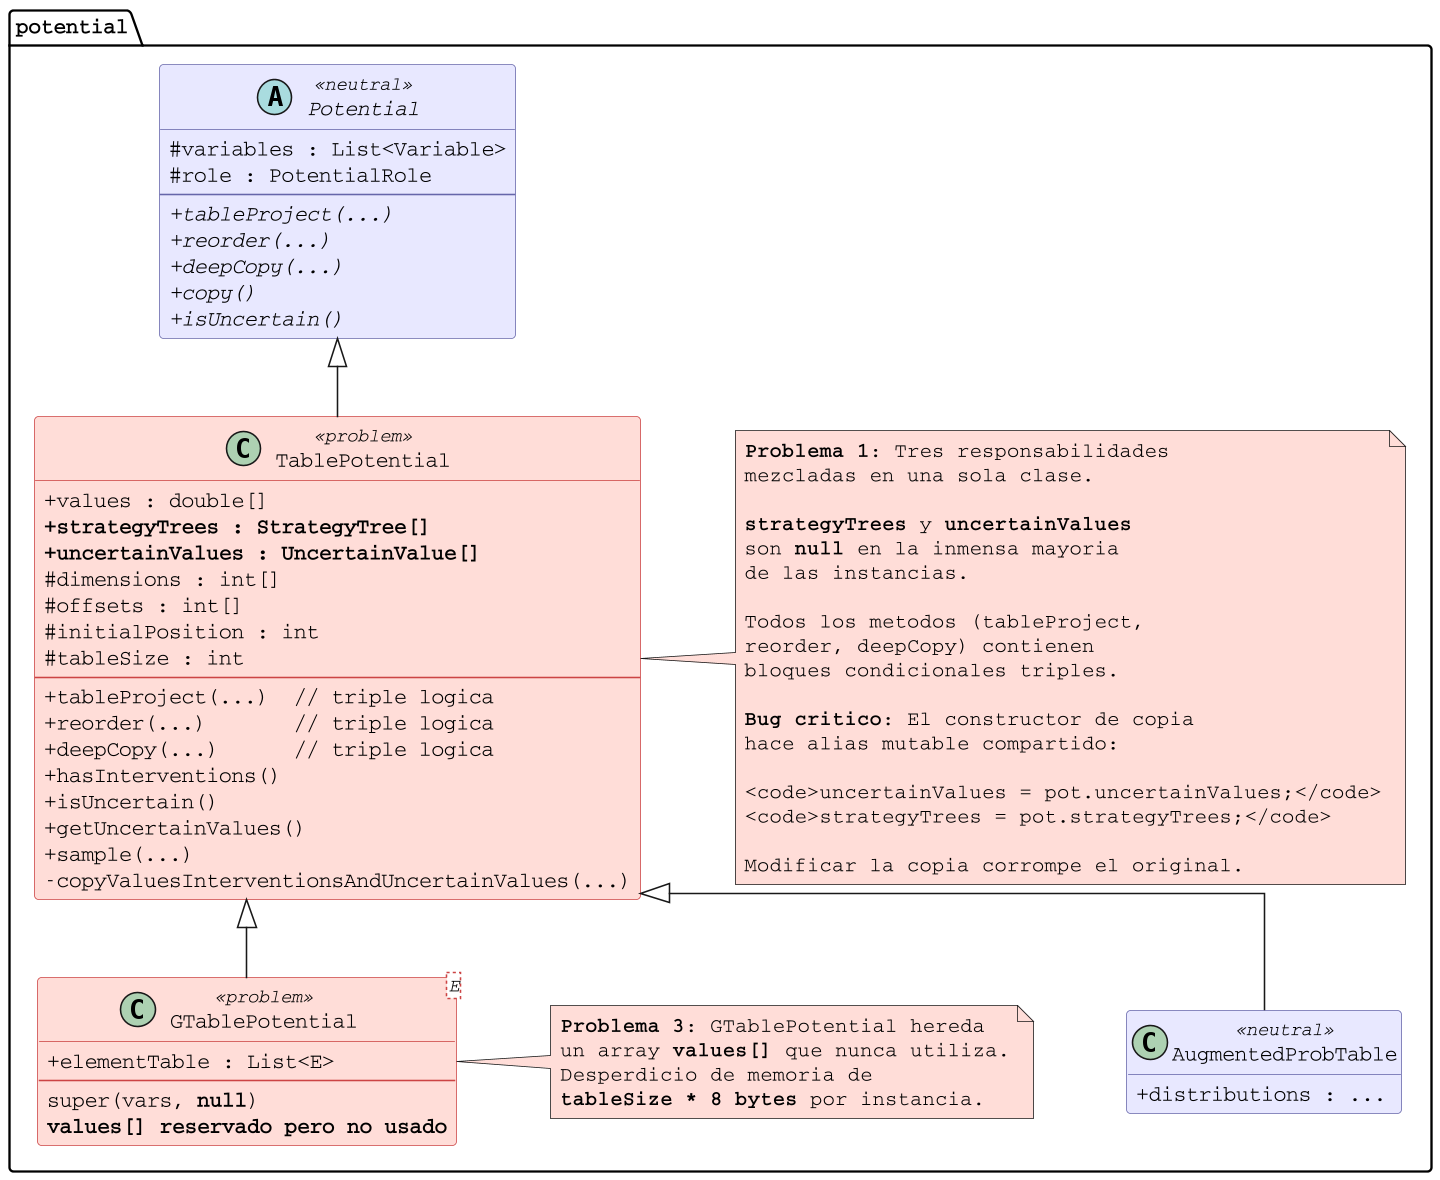
\includegraphics[width=\textwidth]{before.png}
\caption{Jerarquía de \code{TablePotential} antes del rediseño.
         Las clases en rojo presentan problemas de diseño.
         Nótese que \code{TablePotential} contiene tres campos de datos
         (\code{values}, \code{strategyTrees}, \code{uncertainValues}) y que
         \code{GTablePotential} hereda un \code{values[]} que nunca utiliza.}
\label{fig:before}
\end{figure}

Los problemas visibles en el diagrama son:

\begin{enumerate}
  \item \code{TablePotential} es una clase monolítica con campos para tres
        responsabilidades distintas.  Todos sus métodos contienen lógica
        condicional para manejar los tres casos.
  \item \code{GTablePotential<E>} extiende \code{TablePotential} pero no usa su
        campo \code{values[]}: almacena datos en \code{elementTable} (un
        \code{List<E>}) y pasa \code{null} como \code{PotentialRole} al padre.
  \item No existe separación entre la lógica de indexación (dimensiones,
        offsets) y la lógica de almacenamiento de valores.
\end{enumerate}

% ===================================================================
\section{Jerarquía después del rediseño}
\label{sec:after}

La figura~\ref{fig:after} muestra la jerarquía resultante tras completar las
fases~1 a~4.  Las clases en \textcolor{codegreen}{verde} son nuevas; las clases
en \textcolor{warnorange}{amarillo} fueron modificadas; las clases en azul claro
permanecen sin cambios.

\begin{figure}[H]
\centering
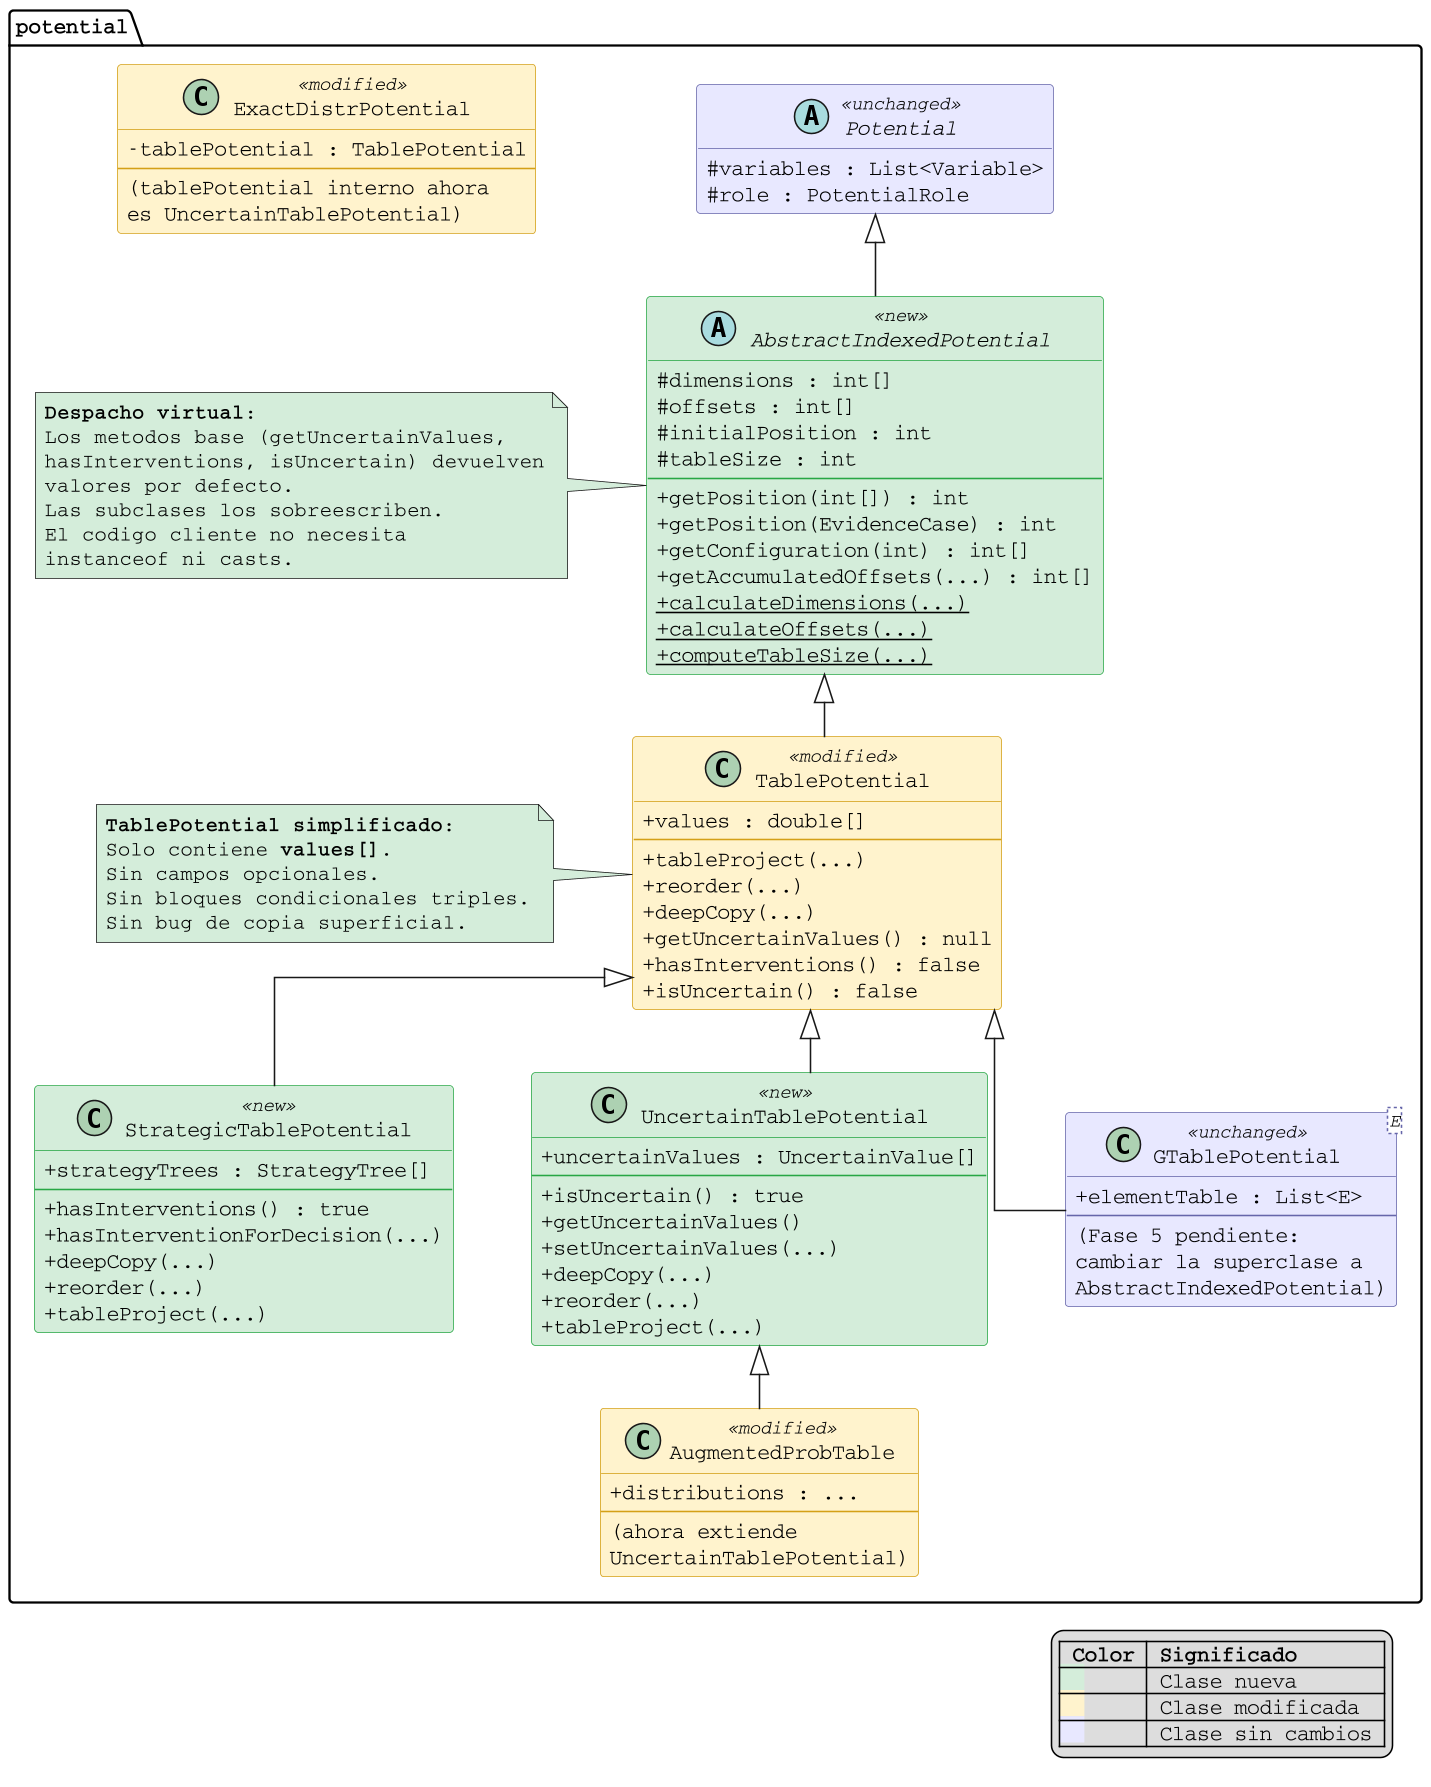
\includegraphics[width=\textwidth]{after.png}
\caption{Jerarquía de \code{TablePotential} después del rediseño (fases 1--4).
         Las clases nuevas (\code{AbstractIndexedPotential},
         \code{StrategicTablePotential}, \code{UncertainTablePotential}) aparecen
         en verde.  Las clases modificadas en amarillo.  \code{GTablePotential}
         sigue extendiendo \code{TablePotential} (fase~5 pendiente).}
\label{fig:after}
\end{figure}

Los cambios fundamentales son:

\begin{enumerate}
  \item \textbf{\code{AbstractIndexedPotential}} (nueva): clase abstracta intermedia
        entre \code{Potential} y \code{TablePotential} que concentra toda la lógica
        de indexación: \code{dimensions[]}, \code{offsets[]}, \code{tableSize},
        \code{initialPosition}, y los métodos estáticos \code{calculateDimensions},
        \code{calculateOffsets}, \code{computeTableSize}.

  \item \textbf{\code{TablePotential}} (simplificado): conserva únicamente el campo
        \code{values[]} y los métodos que operan sobre él.  Sin campos opcionales.
        Sin bloques condicionales triples.

  \item \textbf{\code{StrategicTablePotential}} (nueva): encapsula
        \code{strategyTrees[]} y sobreescribe \code{deepCopy()}, \code{reorder()},
        \code{tableProject()} y \code{hasInterventions()}.  Solo se instancia
        durante la resolución de diagramas de influencia.

  \item \textbf{\code{UncertainTablePotential}} (nueva): encapsula
        \code{uncertainValues[]} y sobreescribe los métodos correspondientes.
        Solo se instancia durante el análisis de sensibilidad paramétrica.

  \item \textbf{\code{AugmentedProbTable}} (modificada): ahora extiende
        \code{UncertainTablePotential} en lugar de \code{TablePotential}, porque
        siempre necesita \code{uncertainValues[]}.

  \item \textbf{\code{ExactDistrPotential}} (modificada): su campo interno
        \code{tablePotential} se crea como \code{UncertainTablePotential} para que
        \code{setUncertainValues()} funcione correctamente por despacho virtual.
\end{enumerate}

% ===================================================================
\section{Detalle de las fases completadas}
\label{sec:fases}

\subsection{Fase 0: Verificación de la línea base}

Antes de cualquier modificación se ejecutaron los 337 tests del módulo
\code{core}:

\begin{lstlisting}[language=bash, caption={Verificación de la línea base}]
cd org.openmarkov.core && mvn clean test
# Tests run: 337, Failures: 0, Errors: 0, Skipped: 10
\end{lstlisting}

Este resultado establece la línea base contra la que se verifican todas las
fases siguientes.

\subsection{Fase 1: Creación de \code{AbstractIndexedPotential}}

\textbf{Objetivo:} Extraer la lógica de indexación de \code{TablePotential} a
una clase abstracta intermedia, preparando el terreno para las fases siguientes y
para la futura cambio de superclase de \code{GTablePotential}.

\textbf{Acciones:}
\begin{enumerate}
  \item Crear \code{AbstractIndexedPotential} como clase abstracta que extiende
        \code{Potential}.
  \item Mover los campos \code{dimensions[]}, \code{offsets[]},
        \code{initialPosition}, \code{tableSize} de \code{Table\-Potential} al
        padre.
  \item Mover los métodos estáticos de cálculo (\code{calculate\-Dimensions},
        \code{calculate\-Offsets}, \code{compute\-Table\-Size},
        \code{get\-Accumulated\-Offsets}, \code{get\-Next\-Position}) y los métodos de
        instancia (\code{get\-Position}, \code{get\-Configuration},
        \code{get\-Accumulated\-Offsets(List)},
        \code{get\-Projected\-Accumulated\-Offsets}).
  \item Cambiar \code{TablePotential extends Potential} a
        \code{Table\-Potential extends Abstract\-Indexed\-Potential}.
\end{enumerate}

\textbf{Ficheros creados:}
\begin{itemize}
  \item \code{potential/AbstractIndexedPotential.java}
\end{itemize}

\textbf{Ficheros modificados:}
\begin{itemize}
  \item \code{potential/TablePotential.java} --- eliminación de campos y métodos
        movidos al padre.
\end{itemize}

\textbf{Verificación:} 337 tests, 0 fallos.

\subsection{Fase 2: Extracción de \code{StrategicTablePotential}}

\textbf{Objetivo:} Extraer el campo \code{strategyTrees[]} y toda su lógica
asociada de \code{TablePotential} a una nueva subclase.

\textbf{Acciones:}
\begin{enumerate}
  \item Crear \code{StrategicTablePotential extends TablePotential} con el campo
        \code{strategyTrees[]}.
  \item Sobreescribir \code{deepCopy()}, \code{reorder()},
        \code{tableProject()}, \code{hasInterventions()},
        \code{has\-Intervention\-For\-Decision()}.
  \item Eliminar de \code{TablePotential} el campo \code{strategyTrees}, el método
        privado
        \code{copy\-Values\-Interventions\-And\-Uncertain\-Values()}, y todos los
        bloques \code{if (strategyTrees != null)}.
  \item Actualizar las clases del paquete \code{operation/} que acceden a
        \code{strategyTrees}: usar \code{instanceof StrategicTablePotential} para
        lecturas, crear \code{StrategicTablePotential} para resultados con
        intervenciones.
\end{enumerate}

\textbf{Clases del paquete \code{operation/} actualizadas:}
\begin{itemize}
  \item \code{MaxOutVariable} --- crea \code{StrategicTablePotential} para la salida;
        usa \code{instanceof} para leer \code{strategyTrees} de la entrada.
  \item \code{SumOutVariable} --- mismo patrón.
  \item \code{TablePotentialElimination} --- mismo patrón.
  \item \code{TablePotentialArithmetic} --- 18+ ocurrencias actualizadas.
  \item \code{TablePotentialTransform} --- clona \code{strategyTrees} via cast.
  \item \code{TablePotentialMerge} --- crea resultado
        \code{StrategicTablePotential} cuando hay intervenciones.
\end{itemize}

\textbf{Ficheros creados:}
\begin{itemize}
  \item \code{potential/StrategicTablePotential.java}
\end{itemize}

\textbf{Verificación:} 337 tests, 0 fallos.

\subsection{Fase 3: Extracción de \code{UncertainTablePotential}}

\textbf{Objetivo:} Extraer el campo \code{uncertainValues[]} y toda su lógica
asociada a una nueva subclase.

\textbf{Acciones:}
\begin{enumerate}
  \item Crear \code{Uncertain\-Table\-Potential}, subclase de
        \code{Table\-Potential}, con el campo propio
        \code{uncertainValues[]}.
  \item Sobreescribir \code{getUncertainValues()}, \code{setUncertainValues()},
        \code{deepCopy()}, \code{reorder(List)}, \code{reorder(Variable, State[])},
        \code{tableProject()}, \code{copy()}.
  \item Mover \code{set\-Uncertain\-Table\-To\-Null\-If\-Null\-Values()} a
        \code{Uncertain\-Table\-Potential} como método estático privado
        \code{nullify\-If\-All\-Null()}.
  \item Simplificar en \code{Table\-Potential}: \code{get\-Uncertain\-Values()}
        devuelve \code{null}; \code{set\-Uncertain\-Values(null)} es un no-op;
        \code{set\-Uncertain\-Values(non-null)} lanza
        \code{Unsupported\-Operation\-Exception}.
  \item Cambiar \code{AugmentedProbTable} para que extienda
        \code{UncertainTablePotential} en lugar de \code{TablePotential}.
  \item Actualizar \code{ExactDistrPotential}: su campo interno
        \code{tablePotential} se crea como \code{UncertainTablePotential}.
  \item Actualizar \code{Table\-Potential\-Sampler}: la tabla muestreada se crea como
        \code{Uncertain\-Table\-Potential}.
  \item Actualizar \code{TreeADDPotential}: accede a \code{uncertainValues} via
        \code{getUncertainValues()} y crea \code{UncertainTablePotential} para el
        resultado cuando hay incertidumbre.
  \item Actualizar \code{SystematicSampling}: crea \code{UncertainTablePotential}
        al replicar valores con incertidumbre.
  \item Actualizar \code{ProbNetOperations}: usa \code{instanceof
        UncertainTablePotential} para acceder a \code{uncertainValues} al
        completar tablas con proyecciones.
\end{enumerate}

\textbf{Caso especial: intervenciones e incertidumbre simultáneas.}
En teoría, un potencial podría necesitar tanto \code{strategyTrees[]} como
\code{uncertainValues[]}.  Sin embargo, la herencia simple de Java impide que
una clase extienda simultáneamente \code{StrategicTablePotential} y
\code{UncertainTablePotential}.  En la práctica, esta combinación es
extremadamente rara (mezclar resolución de IDs con análisis de sensibilidad).
La decisión de diseño fue: cuando ambos están presentes, se usa
\code{StrategicTablePotential} y los valores de incertidumbre no se propagan.
Los métodos de \code{TreeADDPotential} y \code{TablePotentialMerge} documentan
este comportamiento.

\textbf{Ficheros creados:}
\begin{itemize}
  \item \code{potential/UncertainTablePotential.java}
\end{itemize}

\textbf{Ficheros modificados (fuentes principales):}
\begin{itemize}
  \item \code{potential/TablePotential.java}
  \item \code{potential/AugmentedProbTable.java}
  \item \code{potential/ExactDistrPotential.java}
  \item \code{potential/treeadd/TreeADDPotential.java}
  \item \code{potential/operation/TablePotentialMerge.java}
  \item \code{modelUncertainty/SystematicSampling.java}
  \item \code{modelUncertainty/TablePotentialSampler.java}
  \item \code{network/ProbNetOperations.java}
\end{itemize}

\textbf{Ficheros de test modificados:}
\begin{itemize}
  \item \code{test/.../SensitivityAnalysisFactory.java} --- los
        potenciales con \code{uncertainValues} se crean como
        \code{UncertainTablePotential}.
  \item \code{test/.../TablePotentialRegressionTest.java} --- test
        \code{is\-Uncertain\-True\-When\-Uncertain\-Values\-Assigned} actualizado.
\end{itemize}

\textbf{Verificación:} 337 tests, 0 fallos.

\subsection{Fase 4: Actualización de las clases de operaciones}

La actualización de las clases del paquete \code{operation/} se realizó de
forma integrada durante las fases~2 y~3, no como una fase separada.  Cada clase
fue actualizada inmediatamente después de crear la subclase correspondiente,
verificando los tests tras cada cambio.

El patrón general de migración fue:

\begin{lstlisting}[caption={Patrón de migración en las clases de operaciones}]
// ANTES: acceso directo al campo en TablePotential
if (potential.strategyTrees != null) {
    result.strategyTrees = new StrategyTree[size];
    // ...
}

// DESPUES: instanceof + campo en la subclase
if (potential instanceof StrategicTablePotential stp) {
    StrategicTablePotential result = new StrategicTablePotential(vars, role);
    result.strategyTrees = new StrategyTree[size];
    // ...
}
\end{lstlisting}

\textbf{Verificación:} 337 tests, 0 fallos.

% ===================================================================
\section{Fase 5: Cambiar la superclase \code{GTablePotential} (realizada)}
\label{sec:fase5}

La fase~5 completa el Rediseño~1 cambiando \code{GTablePotential<E>} para que
extienda \code{AbstractIndexedPotential} en lugar de \code{TablePotential},
eliminando el array \code{values[]} heredado que nunca se utiliza y corrigiendo
el almacenamiento del rol.  La figura~\ref{fig:phase5} muestra la jerarquía
propuesta; la figura~\ref{fig:phase5-impl} recoge el estado tras la
implementación con el \emph{ripple} de API asociado.

\begin{figure}[H]
\centering
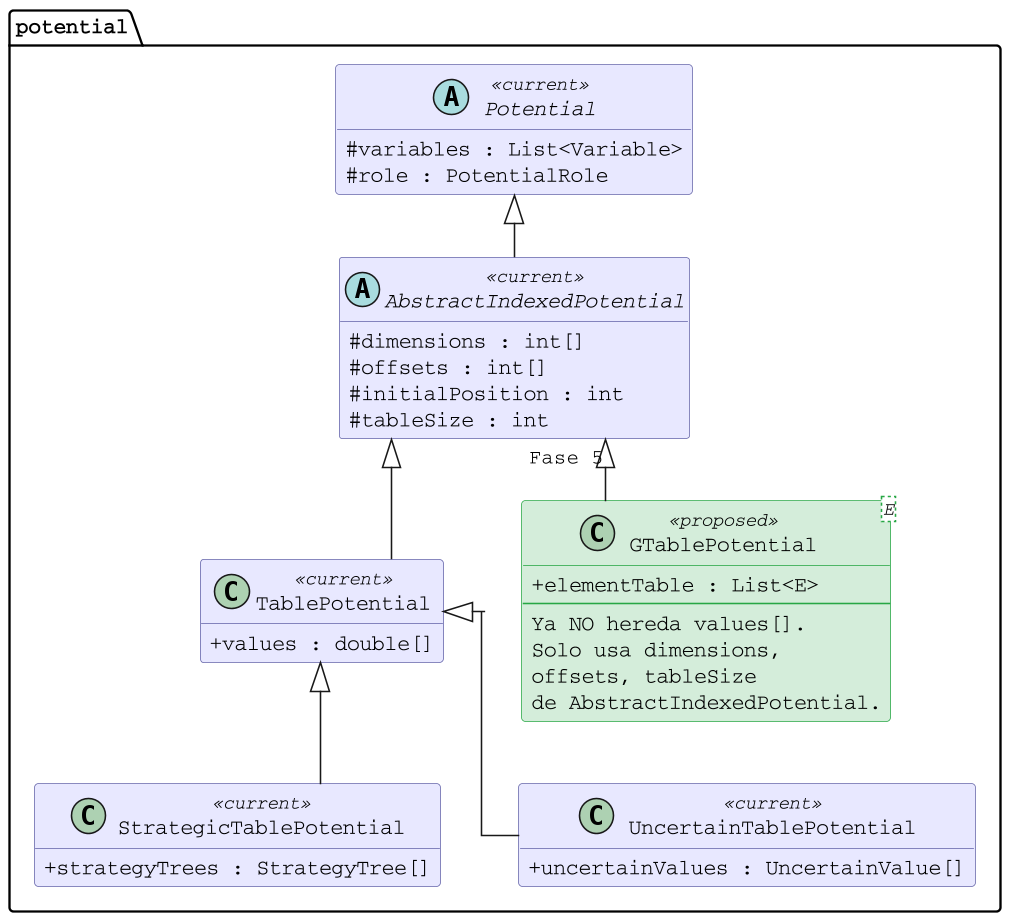
\includegraphics[width=\textwidth]{phase5-proposed.png}
\caption{Fase~5 propuesta: \code{GTablePotential} extiende directamente
         \code{AbstractIndexedPotential}, sin heredar \code{values[]}.
         En verde la clase que cambiaría de padre.}
\label{fig:phase5}
\end{figure}

\subsection{Ventajas del cambio de superclase}
\label{sec:fase5-pros}

\begin{itemize}
  \item \textbf{Ahorro de memoria}: cada instancia de \code{GTablePotential} deja de
        reservar un \code{double[tableSize]} inútil, ahorrando
        \code{tableSize $\times$ 8} bytes por instancia.
  \item \textbf{Jerarquía más limpia}: \code{GTablePotential} \textbf{no es-un}
        \code{TablePotential} en sentido semántico (no almacena \code{double}),
        por lo que la herencia actual viola LSP.  Cambiar la superclaselo corrige esta
        violación.
  \item \textbf{Eliminación del \code{null} forzado}: el constructor ya no
        necesita pasar \code{null} como \code{PotentialRole} al padre para evitar
        la inicialización de \code{values[]}.
\end{itemize}

\subsection{Inconvenientes y motivos del aplazamiento}

\begin{itemize}
  \item \textbf{Rotura de API en \code{Table\-Potential\-Merge.\-merge()}}: este
        método acepta \code{List<\-Table\-Potential>} como parámetro.  Si
        \code{GTablePotential} ya no es subtipo de \code{TablePotential}, los
        objetos \code{GTablePotential} no pueden estar en esa lista.  La
        verificación \code{there\-Are\-GTable\-Potentials()} dentro de
        \code{merge()} se basa en que los \code{GTablePotential} llegan en la
        lista de \code{TablePotential}.  Habría que cambiar la firma a
        \code{List<? extends Abstract\-Indexed\-Poten\-tial>} o introducir una
        indirección adicional.

  \item \textbf{Cascada en \code{Discrete\-Potential\-Operations}}: la fachada
        pública \code{Discrete\-Potential\-Operations.\-merge()} delega en
        \code{Table\-Potential\-Merge.\-merge()}.  Cambiar la firma interna propagaría
        el cambio a la firma pública, afectando a todos los llamadores en
        los módulos \code{inference}, \code{gui} y \code{costEffectiveness}.

  \item \textbf{Cascada en \code{TablePotentialMaximization}}: el método
        \code{multiplyAndMaximize()} crea un \code{GTablePotential<Choice>} como
        segundo resultado devuelto en un \code{Object[]}.  La lógica interna
        accede a \code{potential.values} para todos los potenciales de entrada.
        Si \code{GTablePotential} entra como input sin tener \code{values}, el
        código fallaría.

  \item \textbf{Alto riesgo de regresión}: los cambios afectan al flujo crítico
        de inferencia y requieren una verificación exhaustiva con los tests de
        integración del módulo \code{inference}, además de los 337 tests de
        \code{core}.

  \item \textbf{Beneficio limitado}: en la práctica, el número de instancias de
        \code{GTablePotential} en memoria durante una sesión típica de
        OpenMarkov es pequeño (del orden de decenas, no de miles).  El ahorro
        de memoria, aunque correcto en principio, no justifica el riesgo.
\end{itemize}

\subsection{Condiciones para retomar la fase~5}

La fase~5 debería retomarse cuando se cumpla alguna de estas condiciones:

\begin{itemize}
  \item \textbf{[\checkmark~Satisfecha]} Se emprenda una refactorización más
        amplia de las firmas de \code{Discrete\-Potential\-Operations}: la
        preparación de tests (\code{testMerge},
        \code{test\-Multiply\-And\-Maximize\_*}) ha implicado analizar y reescribir
        en profundidad los tests de \code{Table\-Potential\-Merge} y
        \code{Table\-Potential\-Maximization}, incluyendo la detección del no
        determinismo en \code{variables\-To\-Keep} (construido con \code{HashSet}) y
        la corrección del bug en \code{Choice.\-addValue()}.  Este trabajo sienta
        la base para acometer el cambio de firmas hacia
        \code{List<? extends Abstract\-Indexed\-Potential>} en una próxima fase.
  \item \textbf{[\checkmark~Satisfecha]} Se decidió acometer la cambio de superclase
        una vez completada la preparación de tests, sin necesidad de esperar a
        detectar un escenario de alto uso de memoria; el beneficio arquitectónico
        (corrección de la violación LSP) justificaba el cambio.
  \item \textbf{[\checkmark~Satisfecha]} Se disponga de tests que cubran adecuadamente
        los flujos de \code{merge}, \code{multiplyAndMaximize} y CEA con
        \code{GTablePotential} (véase la sección~\ref{sec:fase5-tests}).
\end{itemize}

% ===================================================================
\subsection{Preparación de tests para la fase~5 (realizada)}
\label{sec:fase5-tests}

Como paso previo a acometer la cambio de superclase se ha completado la cobertura de
tests exigida por la condición~3.  Los trabajos afectan a cuatro clases de test
en dos módulos (\code{core} e \code{integrationtests}) y han requerido corregir
un bug en el código de producción.

\subsubsection*{Bug corregido en producción: \code{Choice.addValue()}}

El método \code{Choice.addValue(int)} tenía una rama \code{else} defectuosa
que se activaba cuando \code{initialized == true} (tras llamar a
\code{setValue()}): escribia \code{values[0] = value} sin incrementar
\code{numValues} ni ampliar el array, de modo que los estados empatados en
utilidad se descartaban y sólo sobrevivía el último.  Esto afectaba
directamente al resultado de \code{multiplyAndMaximize()} en presencia de empates.

La corrección unifica la lógica: \code{addValue()} siempre realloca el array
a \code{numValues + 1}, copia los valores existentes y añade el nuevo al final.
El flag \code{initialized} queda sin efecto en este método.

\subsubsection*{Tests nuevos en \code{org.openmarkov.core}}

\paragraph{\code{ChoiceTest}} \emph{(clase nueva, 20 tests)}\\
Cubre los dos constructores, \code{setValue}, \code{addValue} sin inicializar y
tras \code{setValue}, \code{copy}, \code{sameInformation}, \code{getStates} y
\code{toString}.  Dos tests verifican el comportamiento que antes fallaba por el
bug de \code{addValue}:
\begin{itemize}
  \item \code{addValueAfterSetValueAppendsNewEntry}: empate de dos estados tras
        \code{setValue}; verifica \code{numValues == 2} y los índices correctos.
  \item \code{addValueAfterSetValueThreeTiesHasThreeEntries}: empate a tres
        estados; verifica \code{numValues == 3}.
\end{itemize}

\paragraph{\code{GTablePotentialTest}} \emph{(clase nueva, 15 tests)}\\
Documenta y verifica el comportamiento actual de \code{GTablePotential<E>},
estableciendo una línea base para detectar regresiónes tras la
cambio de superclase:
\begin{itemize}
  \item El array \code{values[]} se reserva con \code{tableSize} ceros y permanece
        siempre a cero; las operaciones sobre \code{elementTable} no lo modifican.
        Este invariante será la primera señal de ruptura si la cambio de superclase
        no elim\-ina \code{values[]} correctamente.
  \item El parámetro \code{role} pasado al constructor es siempre descartado
        porque el constructor llama a \code{super(variables,\,null)}; tras la
        cambio de superclase este defecto quedará eliminado y los tests de \code{role}
        deberán actualizarse para afirmar el valor correcto en lugar de
        \code{null}.
  \item Dimensiones, offsets y variables heredados de \code{AbstractIndexedPotential}
        son correctos para 1, 2 y 3 variables.
\end{itemize}

\paragraph{\code{DiscretePotentialOperationsTest} --- extensiones}
Se han añadido cuatro tests al fichero existente:
\begin{itemize}
  \item \code{testMerge()}: reemplaza el antiguo stub vacío (\code{// TODO}).
        Incluye cuatro sub-casos: fusión de \code{TablePotential} planos con
        verificación de posicionamiento (\code{D=0,X=0}, etc.); fusión de
        \code{GTablePotential<CEP>} con verificación de que el resultado es
        \code{GTablePotential} y \code{values[]} permanece a cero; caso con
        variable de contexto adicional; y lanzamiento de excepción por tamaños
        incompatibles.
  \item \code{testMultiplyAndMaximize\_choiceTableIsPopulated()}: verifica que el
        segundo elemento del array resultado es un \code{GTablePotential<Choice>}
        válido, con el estado óptimo correcto en la posición~0 (A=2, producto
        0.21 contra 0.02).  Nota: las posiciones más allá de la~0 dependen del
        orden de iteración del \code{HashSet} interno que construye
        \code{variablesToKeep}, por lo que sólo se comprueban mediante aserciones
        estructurales (índice en rango válido).
  \item \code{testMultiplyAndMaximize\_tiedStatesBothRecorded()}: empate de dos
        estados; verifica \code{numValues == 2} en el \code{Choice} resultante
        (ejercita el bug corregido de \code{addValue}).
  \item \code{testMultiplyAndMaximize\_threeWayTieAllRecorded()}: empate a tres
        estados; verifica \code{numValues == 3}.
\end{itemize}

\subsubsection*{Tests en \code{org.openmarkov.integrationtests}}

\paragraph{\code{DANCEATest} --- extensiones}
Se han añadido dos bloques de aserciones al método compartido
\code{testCEADANEvaluation()}, que ejecutan todos los subtest de CEA con DAN:
\begin{itemize}
  \item \emph{Validez estructural}: coste y efectividad de cada intervalo del CEP
        no son NaN ni Infinito.
  \item \emph{Consistencia del ICER}: para CEPs de un solo umbral positivo, el
        cociente incremental coste/efectividad entre los dos intervalos debe
        coincidir con el umbral declarado (tolerancia del 1\,\%).
\end{itemize}

\paragraph{\code{CEAGlobalAnalysisTest} --- recuperación de tests desactivados}
El fichero tenía nueve tests; seis estaban marcados con \code{@Disabled}.
Se aplicó el criterio \emph{recuperar si es posible, eliminar si no}.

\medskip
\noindent\textbf{Eliminados (3):}
\begin{itemize}
  \item \code{testCHAP}: \code{VECEAnalysis.\-getUtility()} lanza
        \code{Non\-Projectable\-Potential\-Exception\$\-Cannot\-Resolve\-Variable} al
        procesar \texttt{chap.pgmx}; requiere un fix en el motor de inferencia.
  \item \code{testCHAPSV}: mismo error con \texttt{chap-sv.pgmx}.
  \item \code{testChancellorHC}: \code{ClassCastException} interno
        (\code{Tree\-ADD\-Potential} $\to$ \code{Exact\-Distr\-Potential}) al procesar
        \texttt{MID-dmhee-2.5.pgmx}; requiere un fix en el motor de inferencia.
\end{itemize}

\medskip
\noindent\textbf{Recuperados (3):}
\begin{itemize}
  \item \code{testDMHEE47PSA} y \code{testBriggsSA}: son tests PSA
        (Monte~Carlo sin semilla fija).  Los valores esperados estaban desfasados
        y las tolerancias eran insuficientes para la varianza estocástica.  Se
        reemplazan por aserciones estructurales: tamaño correcto del resultado,
        coste y efectividad finitos y no NaN por estrategia.  Se extrae el helper
        privado \code{assertPsaStructuralValidity()} para evitar duplicación.
  \item \code{testHPV}: afirmaba erróneamente 6 estrategias (2
        decisiones~$\times$~3 estados); \code{VECEAnalysis} procesa un nodo de
        decisión a la vez, por lo que con una variable de 2 estados devuelve
        2~CEPs.  Se corrige el recuento y se sustituyen los valores esperados
        hardcodeados por comprobaciones de validez estructural.
\end{itemize}

\subsubsection*{Recuento final de tests}

\begin{center}
\begin{tabular}{lrrr}
\toprule
\textbf{Módulo} & \textbf{Tests} & \textbf{Fallos} & \textbf{Omitidos} \\
\midrule
\code{org.openmarkov.core} (anterior) & 337 & 0 & 10 \\
\code{org.openmarkov.core} (actual)   & 551 & 0 & 10 \\
\midrule
\code{org.openmarkov.integrationtests} & 365 & 0 & 44 \\
\bottomrule
\end{tabular}
\end{center}

Los 10 tests omitidos en \code{core} son preexistentes y no guardan relación
con el trabajo descrito.  Los 44 omitidos en \code{integrationtests} corresponden
principalmente a tests de GUI que requieren entorno gráfico y a tests marcados
con etiquetas de velocidad que se excluyen en la ejecución estándar.

% ===================================================================
\subsection{Implementación de la fase~5}
\label{sec:fase5-impl}

\subsubsection*{Cambios en el código de producción}

\paragraph{\code{GTablePotential.java}}

La clase pasa de \code{extends TablePotential} a
\code{extends Abstract\-Indexed\-Potential}.
Los efectos concretos son:

\begin{itemize}
  \item \textbf{Constructores corregidos}: todos llaman a \code{super(variables,\,role)}
        en lugar de \code{super(variables,\,null)}, de modo que el \code{PotentialRole}
        queda almacenado correctamente por primera vez.
  \item \textbf{Capacidad inicial de \code{elementTable}}: en vez de recomputar
        manualmente \code{dimensions[n{-}1] $\times$ offsets[n{-}1]}, se usa
        directamente \code{this.tableSize} (calculado por
        \code{Abstract\-Indexed\-Potential} en su constructor).
  \item \textbf{Métodos abstractos implementados}: \code{project(\-EvidenceCase)} lanza
        \code{Non\-Projectable\-Potential\-Exception.\-Potential\-Cannot\-Be\-Converted\-To\-A\-Table};
        \code{copy()} devuelve un nuevo \code{GTablePotential} con las mismas
        variables, el mismo rol y una copia superficial de \code{elementTable}.
  \item \textbf{El método \code{toString()} no cambia}: usa \code{dimensions},
        \code{offsets} y \code{getConfiguration()}, todos heredados de
        \code{AbstractIndexedPotential}, por lo que no es necesario modificarlo.
\end{itemize}

\paragraph{\code{TablePotentialMerge.java} y \code{DiscretePotentialOperations.java}}

Al no ser \code{GTablePotential} un subtipo de \code{TablePotential}, los parámetros
de tipo \code{List<TablePotential>} en \code{merge()} ya no pueden aceptar listas de
objetos \code{GTablePotential}.  La solución adopta el \emph{wildcard} más estrecho
que funciona:

\begin{lstlisting}[caption={Firma anterior y nueva de \texttt{merge()}}]
// Antes
static TablePotential merge(Variable decision,
    List<TablePotential> potentials) throws ...

// Despues
static AbstractIndexedPotential merge(Variable decision,
    List<? extends AbstractIndexedPotential> potentials) throws ...
\end{lstlisting}

El tipo de retorno cambia de \code{TablePotential} a \code{AbstractIndexedPotential}
porque el resultado puede ser un \code{GTablePotential} (cuando todos los potenciales
de entrada son \code{GTablePotential}) o un \code{TablePotential} (en el caso habitual).

Dentro del bucle de relleno, se añade un chequeo \code{instanceof}:

\begin{lstlisting}[caption={Bucle de relleno adaptado en \texttt{TablePotentialMerge.merge()}}]
for (int i = 0; i < numPotentials; i++) {
    AbstractIndexedPotential p = potentials.get(i);
    if (p instanceof GTablePotential<?> gtp) {
        tables[i] = new double[gtp.getTableSize()]; // placeholder de ceros
        elementsTables.set(i, ((GTablePotential<CEP>) gtp).elementTable);
    } else {
        TablePotential tp = (TablePotential) p;
        tables[i] = tp.values;
        if (thereArePotentialsWithInterventions) {
            potentialsInterventions[i] = tp instanceof StrategicTablePotential stp
                    ? stp.strategyTrees : null;
        }
        if (thereArePotentialsWithUncertainValues) {
            potentialsUncertainValues[i] = tp.getUncertainValues();
        }
    }
}
\end{lstlisting}

El array \code{tables[]} para los \code{GTablePotential} recibe ceros porque los
valores numéricos nunca se usan cuando el resultado es un \code{GTablePotential}:
el método devuelve \code{new GTablePotential<>(mergedVariables,\,role,\,mergedElementsTable)},
que ignora \code{mergedValues}.

El resto de métodos privados del fichero (\code{getBooleanArray\-Of\-Potentials\-That\-Are\-GTable\-Potentials},
\code{getPotentialsHaveInterventions}, etc.) reciben el mismo ensanchamiento de tipo.

\paragraph{\code{AuxiliaryOperations.java}}

El método \code{getAccumulatedOffsets(List,\,List<Variable>)} amplia su primer
parámetro de \code{List<TablePotential>} a \code{List<? extends Potential>},
ya que internamente solo invoca \code{getVariables()}, disponible en la clase base.

\paragraph{\code{PotentialOperationException.java}}

El constructor y el campo público de
\code{Different\-Sizes\-In\-Potentials\-And\-States} cambian de
\code{Collection<TablePotential>} a
\code{Collection<? extends Abstract\-Indexed\-Potential>}.

\paragraph{\code{DANInference.java} (módulo \code{inference})}

Los tres puntos de llamada a
\code{Discrete\-Potential\-Operations.\-merge()} reciben
una conversión explícita al tipo esperado por el motor:

\begin{lstlisting}[caption={Cast en \texttt{DANInference.java} (los tres sitios son análogos)}]
TablePotential conditionedUtilityPotential =
    (TablePotential) DiscretePotentialOperations.merge(d, childrenUtility);
\end{lstlisting}

El cast es seguro porque \code{childrenUtility} es siempre una
\code{List<TablePotential>} (potenciales de utilidad, nunca \code{GTablePotential}).

\subsubsection*{Diagrama de la jerarquía implementada}

\begin{figure}[H]
\centering
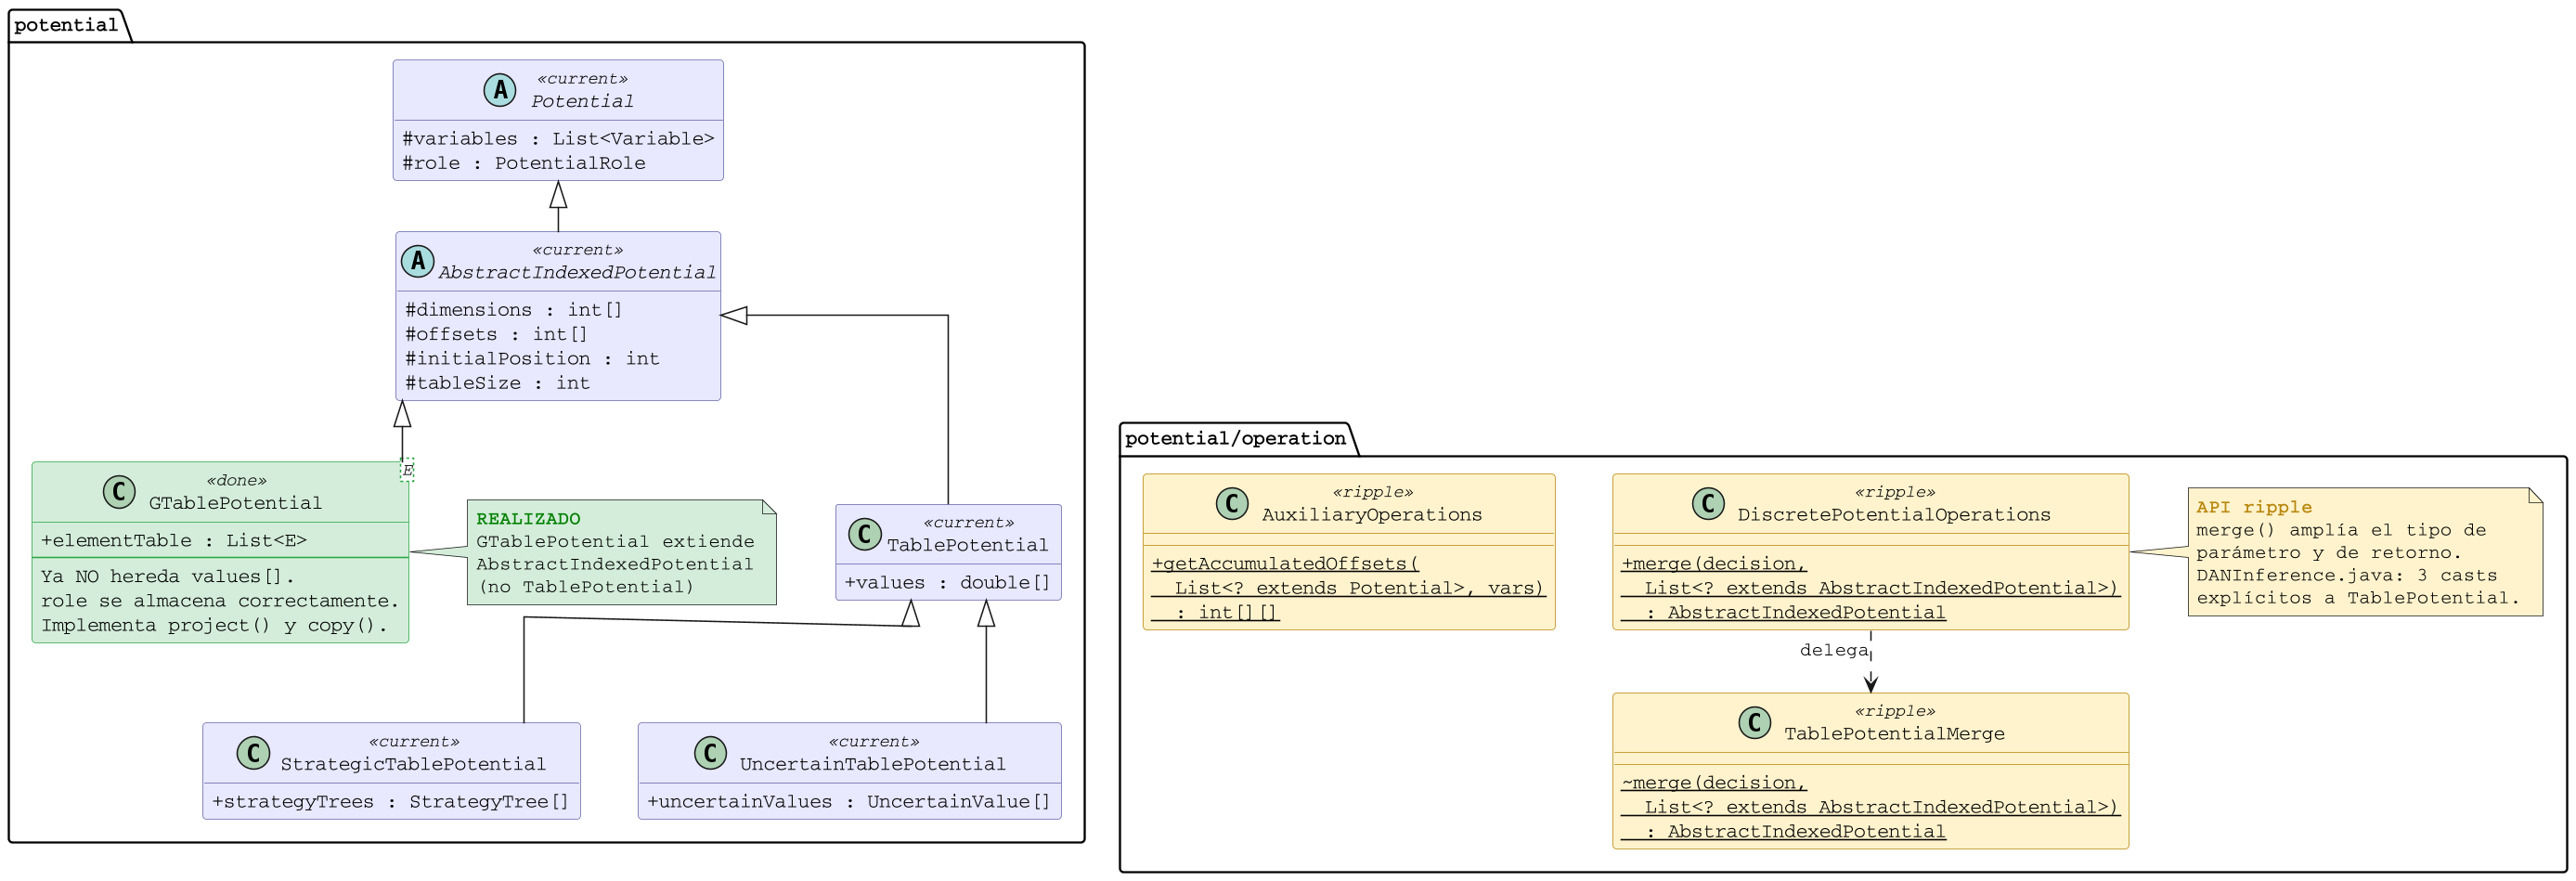
\includegraphics[width=\textwidth]{phase5-implemented.png}
\caption{Estado final de la fase~5: \code{GTablePotential} extiende
         \code{AbstractIndexedPotential} (en verde). Los componentes en amarillo
         son los afectados por el \emph{ripple} de API (\code{merge()} con tipo
         de parámetro y retorno ampliados).}
\label{fig:phase5-impl}
\end{figure}

\subsubsection*{Ventajas observadas tras la implementación}

Las ventajas anticipadas en la sección~\ref{sec:fase5-pros} se confirmaron:

\begin{itemize}
  \item \textbf{Eliminación del \code{values[]} inútil}: cada instancia de
        \code{GTablePotential} deja de reservar el array de \code{double}, ahorrando
        $\mathtt{tableSize} \times 8$~bytes.  En redes de coste-efectividad con
        \code{CEP} completos este ahorro puede ser apreciable.
  \item \textbf{Rol almacenado correctamente}: \code{getPotentialRole()} ya no
        devuelve siempre \code{null}; el parámetro \code{role} del constructor
        se propaga a la clase base.
  \item \textbf{Herencia semánticamente correcta}: \code{GTablePotential}
        \textbf{es-un} \code{Abstract\-Indexed\-Potential} (comparte la lógica de
        indexación multidimensional) pero \textbf{no es-un} \code{TablePotential}
        (no almacena \code{double}), eliminando la violación del principio de
        sustitución de Liskov.
\end{itemize}

\subsubsection*{Inconvenientes materializados}

\begin{itemize}
  \item \textbf{Rotura de compatibilidad de tipo en \code{merge()}}: confirmada.
        Requirió cambiar el tipo de parámetro y de retorno en dos clases
        (\code{Table\-Potential\-Merge}, \code{Discrete\-Potential\-Operations}) más
        tres clases auxiliares (\code{Auxiliary\-Operations},
        \code{Potential\-Operation\-Exception}, \code{DAN\-Inference}).  El cambio es
        mecánico pero toca la API pública de
        \code{Discrete\-Potential\-Operations}.
  \item \textbf{Casts explícitos en el módulo \code{inference}}: los tres puntos
        de llamada en \code{DANInference} necesitan \code{(TablePotential)} delante
        de \code{merge()}.  Son seguros, pero reducen la expresividad del tipo
        estático.  Una alternativa sería sobrecargar \code{merge()} con una
        variante que acepte \code{List<TablePotential>} y devuelva
        \code{TablePotential}; se descartó por aumentar la superficie de la API.
  \item \textbf{Actualización de tests}: los tests que documentaban los defectos
        anteriores (\code{values[]} siempre a cero, \code{role} siempre \code{null})
        debieron invertirse para afirmar el comportamiento correcto.  Cuatro tests
        de \code{GTablePotentialTest} y uno de \code{DiscretePotentialOperationsTest}
        cambiaron de este modo.
  \item \textbf{Inconveniente menor}: \code{TablePotentialMaximization} no
        requirió cambios, pues crea \code{GTablePotential<Choice>} como resultado
        de salida (no como entrada), y los potenciales de entrada siguen siendo
        \code{TablePotential}.
\end{itemize}

\subsubsection*{Recuento final de tests tras la fase~5}

\begin{center}
\begin{tabular}{lrrr}
\toprule
\textbf{Módulo} & \textbf{Tests} & \textbf{Fallos} & \textbf{Omitidos} \\
\midrule
\code{org.openmarkov.core} (tras preparación) & 551 & 0 & 10 \\
\code{org.openmarkov.core} (tras fase~5)         & 552 & 0 & 10 \\
\midrule
\code{org.openmarkov.integrationtests}           & 365 & 0 & 44 \\
\bottomrule
\end{tabular}
\end{center}

El test adicional en \code{core} corresponde a
\code{no\-Role\-Constructor\-Has\-Null\-Role} en \code{GTable\-Potential\-Test},
que verifica que el constructor de un argumento sigue pasando \code{null} como
rol (comportamiento esperado).

% ===================================================================
\section{Verificación y resultados}
\label{sec:verificacion}

\subsection{Tests automáticos}

Tras cada fase se ejecutó la batería completa de tests del módulo \code{core}:

\begin{center}
\begin{tabular}{lccc}
\toprule
\textbf{Fase} & \textbf{Tests ejecutados} & \textbf{Fallos} & \textbf{Omitidos} \\
\midrule
Fase 0 (baseline) & 337 & 0 & 10 \\
Fase 1 (\code{AbstractIndexedPotential}) & 337 & 0 & 10 \\
Fase 2 (\code{StrategicTablePotential}) & 337 & 0 & 10 \\
Fase 3 (\code{UncertainTablePotential}) & 337 & 0 & 10 \\
Fase 4 (operaciones) & 337 & 0 & 10 \\
\midrule
Preparación fase~5 (tests + bug fix) & 551 & 0 & 10 \\
Fase 5 (cambio de superclase \code{GTablePotential}) & 552 & 0 & 10 \\
\bottomrule
\end{tabular}
\end{center}

Los 10 tests omitidos están marcados con \code{@Disabled} en el código fuente
y no están relacionados con los cambios realizados.

\subsection{Impacto pendiente en otros módulos}

Los módulos \code{org.\-openmarkov.\-io} y \code{org.\-openmarkov.\-gui}
contienen código que crea \code{Table\-Potential} y llama a
\code{set\-Uncertain\-Values()} para asignar valores de incertidumbre
leídos de fichero.  Tras el rediseño, estas llamadas deberán crear
\code{Uncertain\-Table\-Potential} en lugar de \code{TablePotential}.  Este cambio está previsto para cuando se aborden dichos
módulos.

Mientras tanto, la compatibilidad hacia atrás está parcialmente preservada:
\code{Table\-Potential.\-set\-Uncertain\-Values(null)} es un no-op (compatible), y
\code{Table\-Potential.\-set\-Uncertain\-Values(non-null)} lanza
\code{Unsupported\-Operation\-Exception} con un mensaje que indica la clase correcta
a usar.

% ===================================================================
\section{Resumen de ficheros afectados}

\begin{table}[H]
\centering
\resizebox{\textwidth}{!}{%
\begin{tabular}{llc}
\toprule
\textbf{Fichero} & \textbf{Acción} & \textbf{Fase} \\
\midrule
\code{potential/AbstractIndexedPotential.java} & Creado & 1 \\
\code{potential/StrategicTablePotential.java} & Creado & 2 \\
\code{potential/UncertainTablePotential.java} & Creado & 3 \\
\midrule
\code{potential/TablePotential.java} & Simplificado & 1--3 \\
\code{potential/AugmentedProbTable.java} & Superclase cambiada & 3 \\
\code{potential/ExactDistrPotential.java} & Modificado & 3 \\
\code{potential/treeadd/TreeADDPotential.java} & Modificado & 3 \\
\midrule
\code{potential/operation/MaxOutVariable.java} & Modificado & 2 \\
\code{potential/operation/SumOutVariable.java} & Modificado & 2 \\
\code{potential/operation/TablePotentialElimination.java} & Modificado & 2 \\
\code{potential/operation/TablePotentialArithmetic.java} & Modificado & 2 \\
\code{potential/operation/TablePotentialTransform.java} & Modificado & 2 \\
\code{potential/operation/TablePotentialMerge.java} & Modificado & 2--3 \\
\midrule
\code{modelUncertainty/SystematicSampling.java} & Modificado & 3 \\
\code{modelUncertainty/TablePotentialSampler.java} & Modificado & 3 \\
\code{network/ProbNetOperations.java} & Modificado & 3 \\
\midrule
\code{test/.../SensitivityAnalysisFactory.java} & Modificado & 3 \\
\code{test/.../TablePotentialRegressionTest.java} & Modificado & 3 \\
\midrule
\multicolumn{3}{l}{\emph{Preparación de tests para la fase~5}} \\
\midrule
\code{inference/Choice.java} & Bug corregido (\code{addValue}) & 5-prep \\
\code{test/.../ChoiceTest.java} & Creado (20 tests) & 5-prep \\
\code{test/.../GTablePotentialTest.java} & Creado (15 tests) & 5-prep \\
\code{test/.../DiscretePotentialOperationsTest.java} & +4 tests, stub \code{testMerge} & 5-prep \\
\code{integrationtests/.../DANCEATest.java} & +aserciones estructurales e ICER & 5-prep \\
\code{integrationtests/.../CEAGlobalAnalysisTest.java} & 3 tests eliminados, 3 corregidos & 5-prep \\
\midrule
\multicolumn{3}{l}{\emph{Fase~5: cambio de superclase de \code{GTablePotential}}} \\
\midrule
\code{potential/GTablePotential.java} & Superclase cambiada a \code{AbstractIndexedPotential} & 5 \\
\code{potential/operation/TablePotentialMerge.java} & Firma \code{merge()} ampliada & 5 \\
\code{potential/operation/DiscretePotentialOperations.java} & Firma \code{merge()} ampliada & 5 \\
\code{potential/operation/AuxiliaryOperations.java} & Firma \code{getAccumulatedOffsets} ampliada & 5 \\
\code{exception/PotentialOperationException.java} & Tipo campo \code{potentials} ampliado & 5 \\
\code{inference/.../DANInference.java} & Cast explícito en 3 llamadas a \code{merge()} & 5 \\
\code{test/.../GTablePotentialTest.java} & Tests actualizados (valores correctos) & 5 \\
\code{test/.../DiscretePotentialOperationsTest.java} & Tests actualizados & 5 \\
\code{test/.../UtilTestMethods.java} & Firma \code{getConfigurationPosition} ampliada & 5 \\
\bottomrule
\end{tabular}%
}
\caption{Ficheros afectados por el Rediseño~1 y la preparación de la fase~5, organizados por fase.}
\label{tab:ficheros}
\end{table}

% ===================================================================
\section{Próximos pasos: Rediseño 3}
\label{sec:proximos-pasos}

El Rediseño~1 (Opción~1) es deliberadamente conservador: resuelve el problema
más grave (los campos opcionales y el bug de aliasing) sin modificar la
jerarquía de \code{Potential} ni las firmas públicas del motor de inferencia.
Los problemas restantes ---métodos abstractos forzados
(sección~\ref{sec:prob2}), \emph{downcasts} en inferencia
(sección~\ref{sec:prob4}), dependencia cíclica (sección~\ref{sec:prob5}) y
el antipatrón \code{PotentialRole} (sección~\ref{sec:prob6})--- requieren un
rediseño de mayor alcance.

El siguiente paso previsto es el \textbf{Rediseño~3}, basado en la Opción~3
(composición mediante interfaces de capacidad), que abordará estos problemas
residuales.  Su documentación se añadirá como una nueva parte de este
documento cuando se inicie su implementación.

% ===================================================================
% ===================================================================
\newpage
\part{Rediseño 3: Análisis de la Opción 3 (Interfaces de Capacidad)}
\label{part:rediseno3}

% ===================================================================
\section{Introducción y objetivos}
\label{sec:op3-intro}

El Rediseño~1 resolvió el problema más urgente: la presencia de campos
opcionales (\code{strategyTrees[]}, \code{uncertainValues[]}) directamente en
\code{TablePotential}, con el bug de aliasing asociado.  Tras esas cuatro fases,
la jerarquía es más limpia en cuanto a responsabilidades de datos.  Sin
embargo, cuatro problemas estructurales persisten:

\begin{enumerate}
  \item \textbf{Métodos abstractos forzados} (sección~\ref{sec:prob2}): la
        clase base \code{Potential} declara \code{tableProject()}, \code{reorder()}
        y otros métodos como abstractos, obligando a subclases como
        \code{UniformPotential}, \code{DeltaPotential} e \code{ICIPotential} a
        proporcionar implementaciones que devuelven \code{null} o lanzan
        \code{UnsupportedOperationException}.

  \item \textbf{\emph{Downcasts} en inferencia} (sección~\ref{sec:prob4}): el
        módulo \code{org.openmarkov.inference} realiza más de 16 conversiones
        explícitas a \code{TablePotential} o \code{StrategicTablePotential} en
        rutas críticas, con riesgo de \code{ClassCastException} en tiempo de
        ejecución.

  \item \textbf{Dependencia cíclica} (sección~\ref{sec:prob5}):
        \code{Table\-Potential} $\leftrightarrow$ \code{StrategyTree}
        $\leftrightarrow$ \code{Tree\-ADD\-Potential}.

  \item \textbf{Antipatrón \code{PotentialRole} como código de tipo}
        (sección~\ref{sec:prob6}).
\end{enumerate}

La \textbf{Opción~3} propone resolver los dos primeros ---y facilitar el
tercero--- introduciendo \emph{interfaces de capacidad}: en lugar de que la clase
base \code{Potential} declare operaciones que no todas las subclases pueden
implementar correctamente, se definen interfaces especializadas
(\code{Projectable}, \code{Reorderable}, \code{Scalable}, \code{UncertaintyCarrier},
\code{StrategyCarrier}) que cada clase implementa solo si posee esa capacidad.

Esta sección analiza en detalle el diseño propuesto, su impacto sobre los
módulos \code{inference}, \code{gui}, \code{io}, \code{learning} y
\code{costEffectiveness}, los problemas que puede introducir, y concluye con una
recomendación fundada.

% ===================================================================
\section{Estado de partida (tras el Rediseño~1)}
\label{sec:op3-partida}

La figura~\ref{fig:op3-antes} muestra la jerarquía de potenciales en el estado
actual, tras completar las fases~1--4 del Rediseño~1.  Las clases marcadas en
\textcolor{codered}{rojo-rosa} son las que presentan implementaciones
problemáticas de los métodos abstractos heredados.

\begin{figure}[H]
\centering
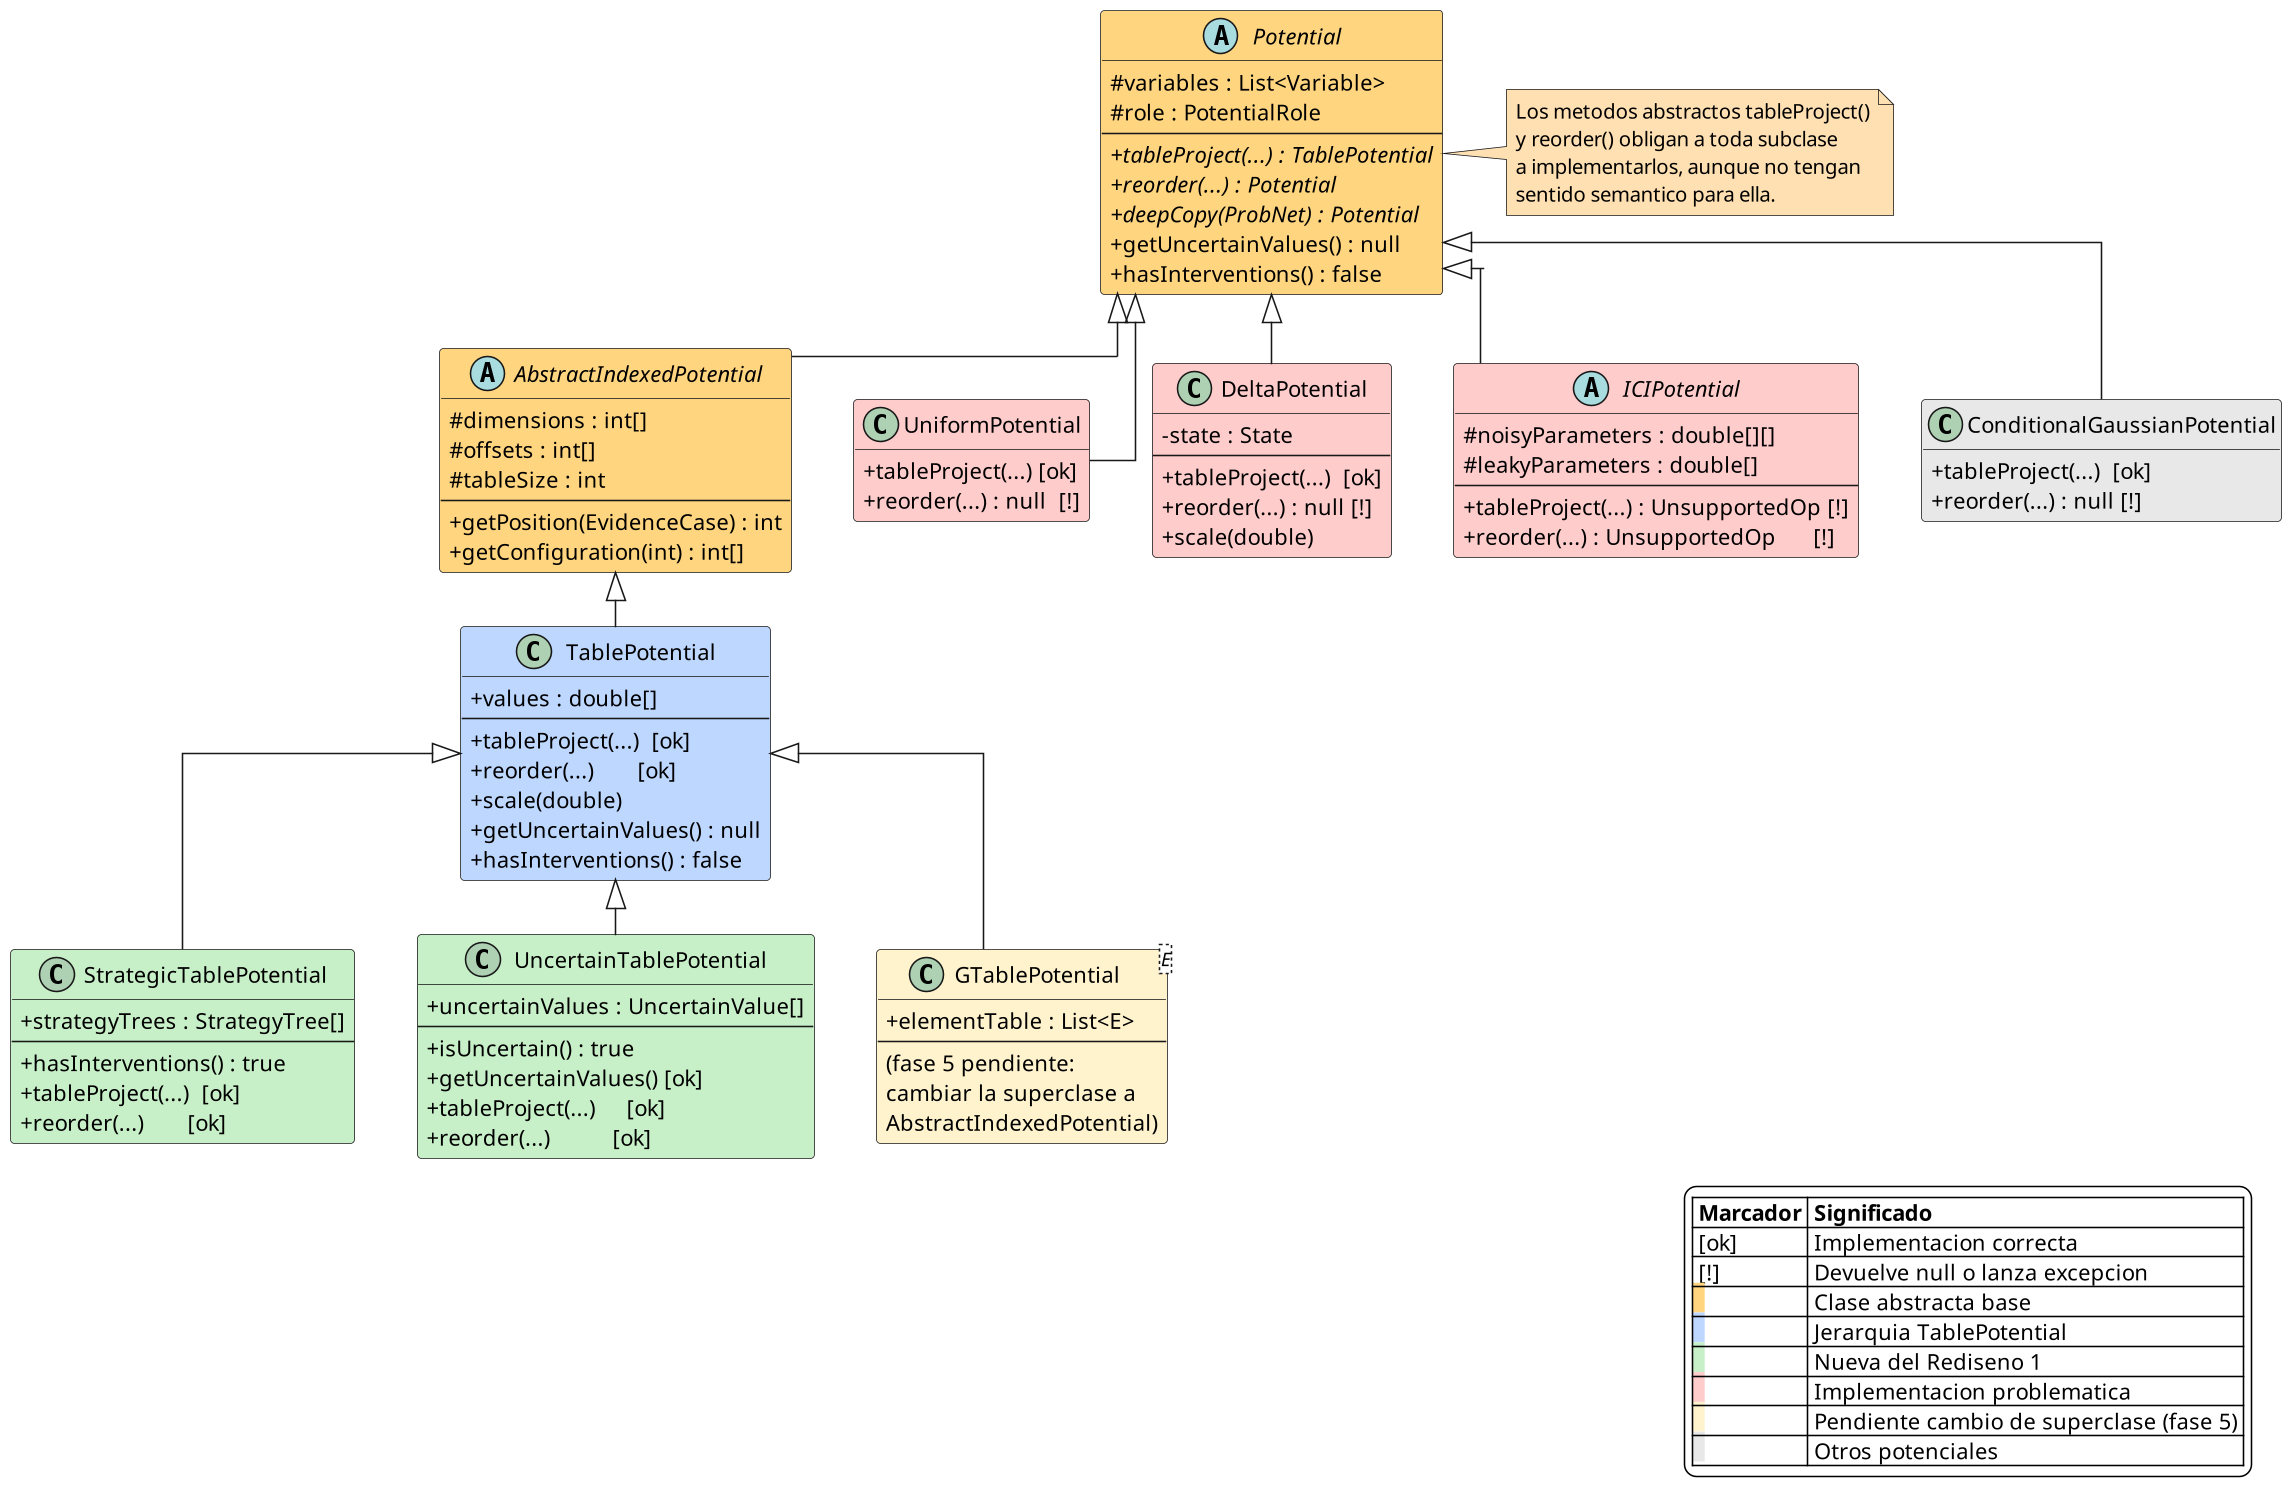
\includegraphics[width=\textwidth]{fig-op3-antes.png}
\caption{Jerarquía de potenciales tras el Rediseño~1.  Las clases en rojo-rosa
         implementan \code{tableProject()} o \code{reorder()} devolviendo
         \code{null} o lanzando \code{UnsupportedOperationException}, porque la
         clase base abstracta \code{Potential} los declara obligatorios aunque no
         tengan sentido semántico para esas subclases.}
\label{fig:op3-antes}
\end{figure}

Las clases marcadas en rojo que no pertenecen a la jerarquía de
\code{TablePotential} evidencian una violación del \emph{Refused Bequest}
(sección~\ref{sec:fund-refused-bequest}): \code{UniformPotential} y
\code{DeltaPotential} implementan \code{reorder()} devolviendo \code{null},
comportamiento indefinido para cualquier llamador que espere un
\code{Potential} válido.  \code{ICIPotential} va más lejos: tanto
\code{tableProject()} como \code{reorder()} lanzan
\code{UnsupportedOperationException}, pese a que la clase base los declara
obligatorios.  En ambos casos la causa raíz es la misma: la clase base
\code{Potential} impone un contrato que sus subclases no pueden cumplir.
\code{ConditionalGaussianPotential} presenta el mismo problema con
\code{reorder()}.

El problema central es que \code{Potential} declara como abstractos métodos que
solo son válidos para la jerarquía \code{TablePotential}:

\begin{lstlisting}[caption={Métodos abstractos problemáticos en la clase base \code{Potential}}]
public abstract TablePotential tableProject(
    EvidenceCase evidence, InferenceOptions options);

public abstract Potential reorder(List<Variable> newOrder);
\end{lstlisting}

Las subclases fuera de la jerarquía \code{TablePotential} no pueden implementar
correctamente estos métodos.  El patrón resultante, que se repite en
\code{UniformPotential}, \code{DeltaPotential} y otros, es el siguiente:

\begin{lstlisting}[caption={Implementación forzada en subclases que no pueden reordenar}]
// DeltaPotential -- no puede reordenar de forma general
@Override
public Potential reorder(List<Variable> newOrder) {
    return null;  // contrato violado: caller puede esperar un Potential valido
}

// ICIPotential -- tableProject no es aplicable al modelo canonico
@Override
public TablePotential tableProject(EvidenceCase ev, InferenceOptions opts) {
    throw new UnsupportedOperationException("ICIPotential no soporta tableProject");
}
\end{lstlisting}

Este patrón viola el \emph{Principio de Substitución de Liskov} (LSP): el
código que llama \code{potential.reorder(vars)} espera recibir un \code{Potential}
válido, no \code{null}.  El código que llama \code{potential.tableProject(ev)}
espera un resultado, no una excepción en tiempo de ejecución.

% ===================================================================
\section{Diseño propuesto: interfaces de capacidad}
\label{sec:op3-propuesta}

La Opción~3 introduce cinco interfaces que encapsulan las operaciones que solo
algunas clases pueden realizar:

\begin{itemize}
  \item \textbf{\code{Projectable}}: puede proyectarse contra una evidencia
        parcial para obtener una \code{TablePotential}.  La operación
        \code{tableProject(EvidenceCase, InferenceOptions)} es el núcleo del
        algoritmo de eliminación de variables en inferencia.

  \item \textbf{\code{Reorderable}}: puede reordenar sus variables internas
        siguiendo un orden especificado, devolviendo un nuevo potencial con la
        misma distribución pero variables en el orden solicitado.  Esencial
        para compatibilidad de índices en operaciones de multiplicación y
        marginalizácion.

  \item \textbf{\code{Scalable}}: puede multiplicar todos sus valores por un
        factor escalar.  Usada en descuentos temporales y normalización de
        utilidades.

  \item \textbf{\code{UncertaintyCarrier}}: almacena y expone distribuciones
        de incertidumbre sobre sus parámetros (\code{UncertainValue[]}).
        Usada en análisis de sensibilidad paramétrica (PSA).

  \item \textbf{\code{StrategyCarrier}}: contiene árboles de estrategia de
        intervención (\code{StrategyTree[]}).  Usada en la resolución de
        diagramas de influencia.
\end{itemize}

\begin{lstlisting}[caption={Definición de las interfaces de capacidad (Opción~3)}]
public interface Projectable {
    TablePotential tableProject(EvidenceCase evidence,
                                InferenceOptions options);
}

public interface Reorderable {
    Potential reorder(List<Variable> newOrderOfVariables);
}

public interface Scalable {
    void scale(double factor);
}

public interface UncertaintyCarrier {
    UncertainValue[] getUncertainValues();
    void setUncertainValues(UncertainValue[] values);
    default boolean isUncertain() { return getUncertainValues() != null; }
}

public interface StrategyCarrier {
    StrategyTree[] getStrategyTrees();
    boolean hasInterventions();
    boolean hasInterventionForDecision(Variable decisionVariable);
}
\end{lstlisting}

Con estas interfaces, la clase base \code{Potential} ya no necesita declarar
\code{tableProject()} ni \code{reorder()} como abstractos.  Cada subclase
implementa únicamente las interfaces que tiene sentido para ella:

\begin{lstlisting}[caption={Declaraciones de clases en la Opción~3}]
// TablePotential: soporta las tres operaciones generales
public class TablePotential extends AbstractIndexedPotential
    implements Projectable, Reorderable, Scalable { ... }

// StrategicTablePotential: ademas soporta estrategias
public class StrategicTablePotential extends TablePotential
    implements StrategyCarrier { ... }

// UncertainTablePotential: ademas soporta incertidumbre
public class UncertainTablePotential extends TablePotential
    implements UncertaintyCarrier { ... }

// UniformPotential: solo puede proyectarse
public class UniformPotential extends Potential
    implements Projectable { ... }

// DeltaPotential: puede proyectarse y escalarse
public class DeltaPotential extends Potential
    implements Projectable, Scalable { ... }

// ICIPotential: puede proyectarse (a una TablePotential de la forma canonica)
public abstract class ICIPotential extends Potential
    implements Projectable { ... }
\end{lstlisting}

El código cliente que necesita una capacidad específica ahora puede
verificar la interfaz en lugar del tipo concreto:

\begin{lstlisting}[caption={Uso de interfaces para eliminar \emph{downcasts} en código cliente}]
// ANTES (con downcast y riesgo de ClassCastException)
TablePotential tp = (TablePotential) potential;
TablePotential projected = tp.tableProject(evidence, opts);

// DESPUES (con interfaz, sin downcast)
if (potential instanceof Projectable proj) {
    TablePotential projected = proj.tableProject(evidence, opts);
}

// O, si el tipo del parametro se declara directamente:
public void processProjectable(Projectable proj, EvidenceCase ev) {
    TablePotential result = proj.tableProject(ev, null);
    // ...
}
\end{lstlisting}

La figura~\ref{fig:op3-despues} muestra el diagrama de clases completo tras
aplicar la Opción~3.

\begin{figure}[H]
\centering
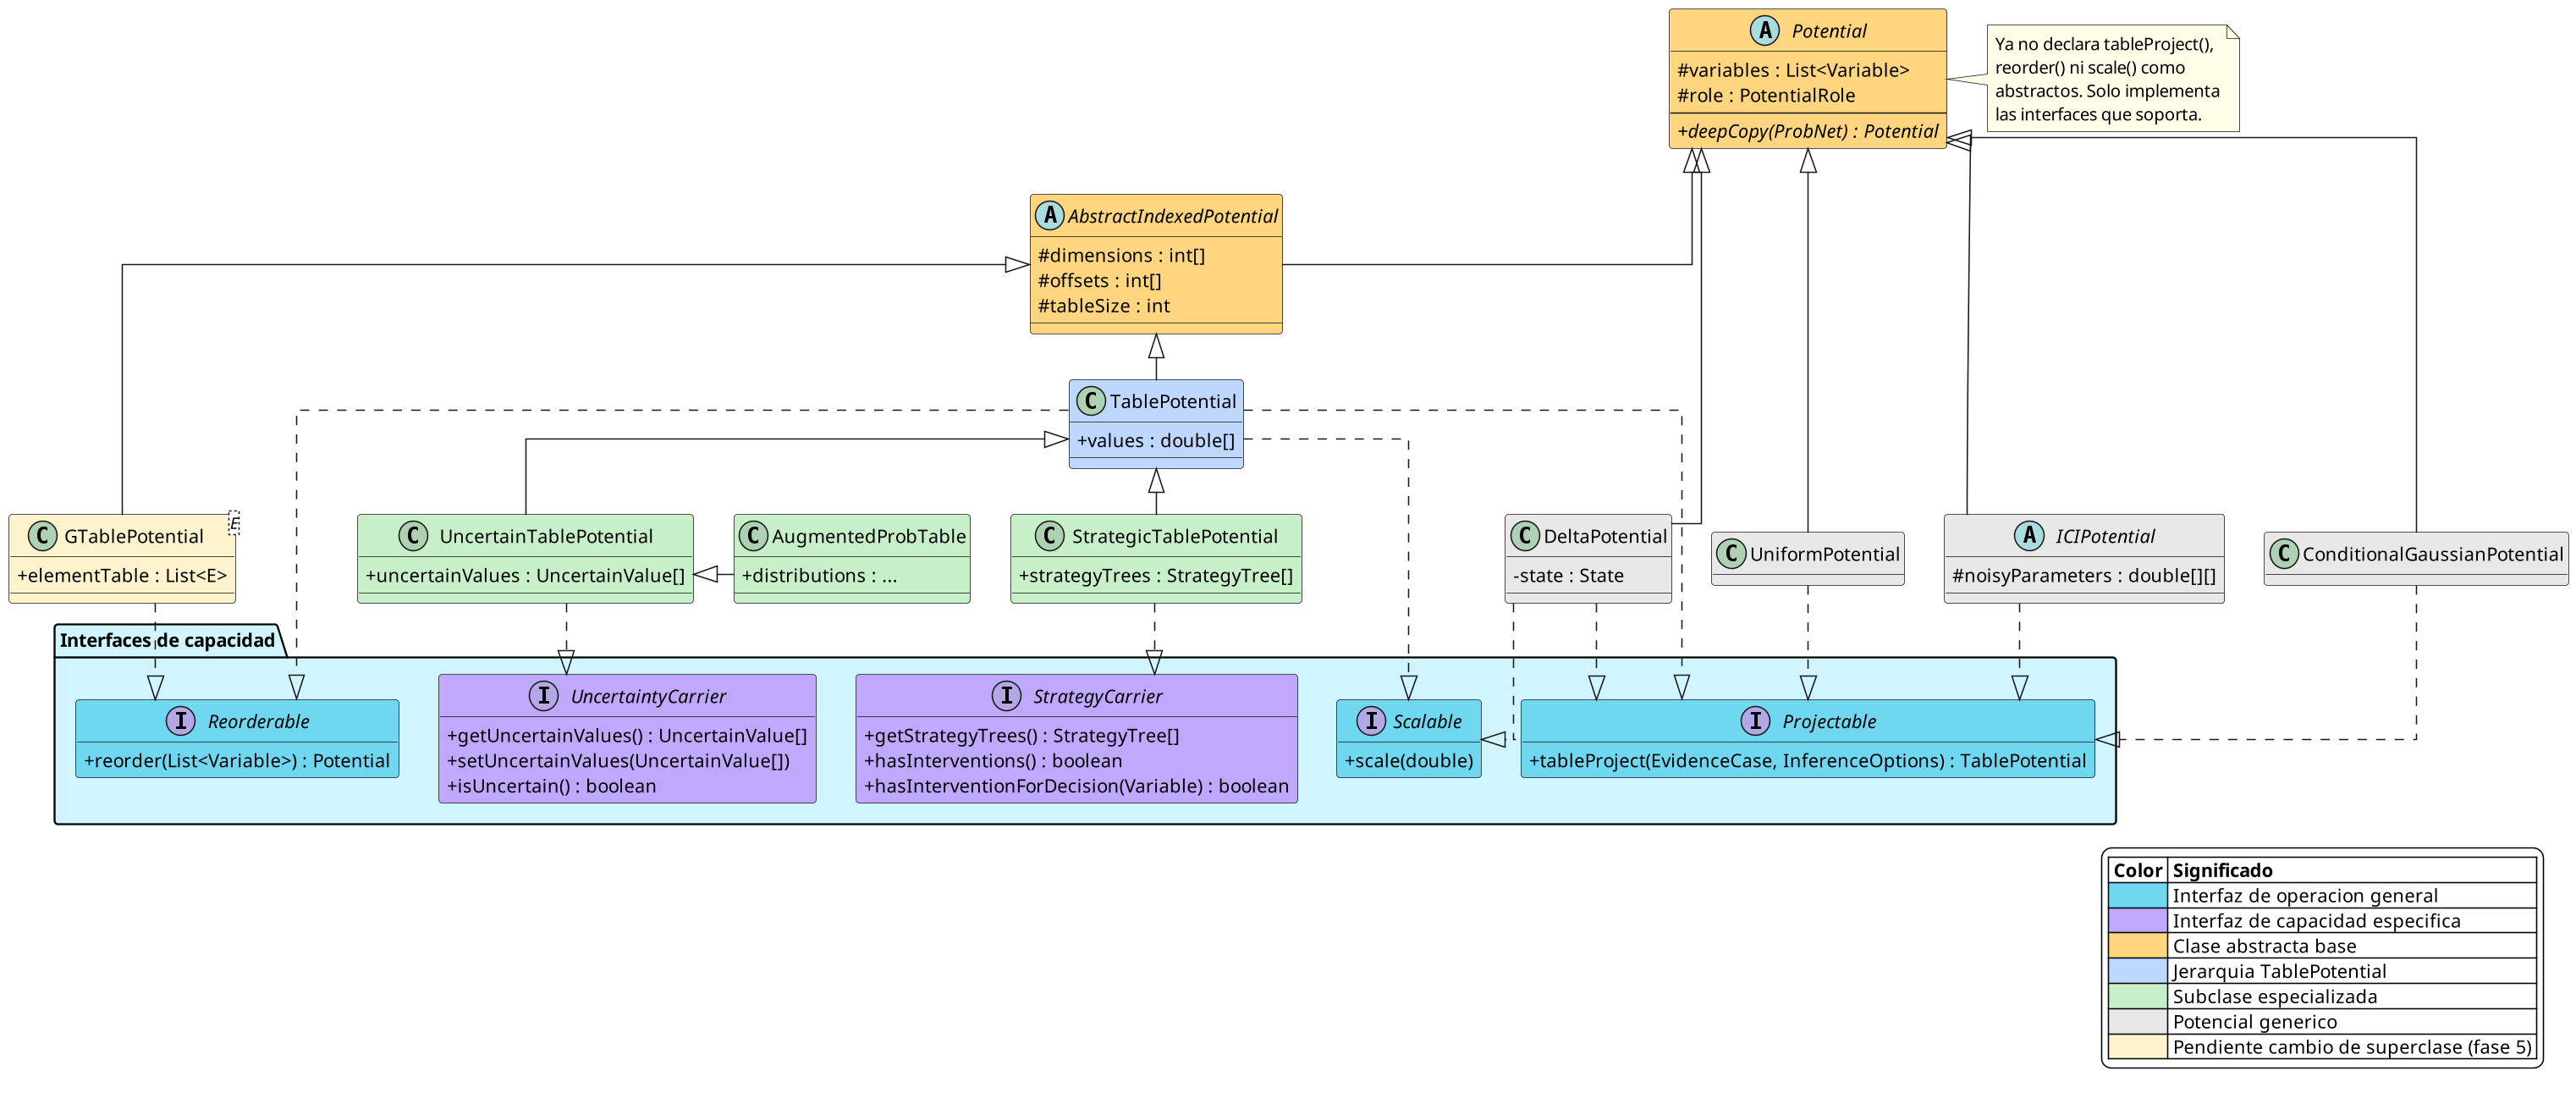
\includegraphics[width=\textwidth]{fig-op3-despues.png}
\caption{Jerarquía propuesta con interfaces de capacidad (Opción~3).
         El paquete azul contiene las cinco interfaces.  Las líneas punteadas
         indican implementación.  La clase base \code{Potential} ya no declara
         \code{tableProject()} ni \code{reorder()} como abstractos: solo las
         clases que verdaderamente soportan esas operaciones implementan la
         interfaz correspondiente.}
\label{fig:op3-despues}
\end{figure}

\subsection{Tabla de implementación de interfaces por clase}
\label{sec:op3-tabla}

La tabla~\ref{tab:op3-interfaces} resume qué interfaces implementa cada tipo
de potencial en el diseño propuesto.  Las columnas representan las cinco
interfaces de capacidad; las filas, las clases de potencial más relevantes.

\newcommand{\yes}{$\checkmark$}
\newcommand{\no}{$-$}

\begin{table}[H]
\centering
\setlength{\tabcolsep}{3pt}
\resizebox{\textwidth}{!}{%
\begin{tabular}{l|ccccc}
\toprule
\textbf{Clase de potencial}
  & \rotatebox{90}{\code{Projectable}\hspace{8pt}}
  & \rotatebox{90}{\code{Reorderable}\hspace{8pt}}
  & \rotatebox{90}{\code{Scalable}\hspace{8pt}}
  & \rotatebox{90}{\code{UncertaintyCarrier}\hspace{8pt}}
  & \rotatebox{90}{\code{StrategyCarrier}\hspace{8pt}} \\
\midrule
\code{TablePotential}             & \yes & \yes & \yes & \no  & \no  \\
\code{StrategicTablePotential}    & \yes & \yes & \yes & \no  & \yes \\
\code{UncertainTablePotential}    & \yes & \yes & \yes & \yes & \no  \\
\code{AugmentedProbTable}         & \yes & \yes & \yes & \yes & \no  \\
\code{GTablePotential<E>}         & \no  & \yes & \no  & \no  & \no  \\
\midrule
\code{UniformPotential}           & \yes & \no  & \no  & \no  & \no  \\
\code{DeltaPotential}             & \yes & \no  & \yes & \no  & \no  \\
\code{ICIPotential}               & \yes & \no  & \no  & \no  & \no  \\
\code{ConditionalGaussianPotential} & \yes & \no & \no & \no  & \no  \\
\code{FunctionPotential}          & \no  & \no  & \no  & \no  & \no  \\
\code{LinearCombinationPotential} & \no  & \no  & \yes & \no  & \no  \\
\code{TreeADDPotential}           & \yes & \no  & \no  & \no  & \yes \\
\code{ExponentialHazardPotential} & \no  & \no  & \no  & \no  & \no  \\
\code{WeibullHazardPotential}     & \no  & \no  & \no  & \no  & \no  \\
\code{GLMPotential}               & \no  & \no  & \no  & \no  & \no  \\
\bottomrule
\end{tabular}%
}
\caption{Implementación de interfaces de capacidad por clase de potencial en
         la Opción~3.  \checkmark{} indica que la clase implementa la interfaz;
         $-$ indica que no la implementa (y no necesita hacerlo).  Las subclases
         heredan las implementaciones de su superclase (por ejemplo,
         \code{StrategicTablePotential} hereda \code{Projectable} de
         \code{TablePotential}).}
\label{tab:op3-interfaces}
\end{table}

% ===================================================================
\section{Análisis de impacto en otros módulos}
\label{sec:op3-impacto}

La Opción~3 afecta a todos los módulos que usan potenciales.  Se ha realizado
una revisión exhaustiva de los cuatro módulos principales: \code{inference},
\code{gui}, \code{io} y \code{learning}.  Los resultados se presentan por módulo,
ordenados de mayor a menor impacto.

\subsection{\code{org.openmarkov.inference} (impacto alto)}
\label{sec:op3-inference}

El módulo de inferencia es el mayor consumidor de las operaciones afectadas
por la Opción~3.  Se han identificado los siguientes puntos de cambio:

\begin{itemize}
  \item \textbf{16+ conversiones (\emph{casts}) a \code{TablePotential}} en rutas
        críticas: \code{VariableEliminationCore} concentra 8 de ellas en los
        métodos de multiplicación y marginalización.  Con las interfaces,
        muchas de estas conversiones dejarían de ser necesarias si los parámetros
        y retornos se declaran con el tipo de interfaz adecuado.

  \item \textbf{6 llamadas a \code{tableProject()}} en los algoritmos de propagación
        y evaluación temporal (\code{VEPropagation}, \code{DANOperations},
        \code{TemporalEvaluation}, \code{MIDTemporalEvolution}).  Actualmente se
        llaman sobre variables declaradas como \code{Potential} tras un cast
        implícito.  Con \code{Projectable}, estas llamadas serían directas.

  \item \textbf{6 llamadas a \code{reorder()}} en eliminación de variables y
        análisis de sensibilidad (\code{Chance\-Variable\-Elimination},
        \code{VE\-Expected\-Utility\-Decision}, \code{VESensAnPlot},
        \code{VE\-Sens\-An\-Tornado\-Spider}, \code{VESensAnMap},
        \code{MID\-Temporal\-Evolution}).  Actualmente devuelven \code{Potential}
        y se reasignan a variables \code{TablePotential} con cast.

  \item \textbf{1 llamada a \code{scale()}} en \code{MIDTemporalEvolution} para
        descuento temporal de utilidades.

  \item \textbf{Acceso directo al campo \code{strategyTrees}} en
        \code{VEOptimalIntervention} y \code{VEEvaluation}: se crea una nueva
        \code{StrategicTablePotential} cuando una utilidad tiene intervenciones.
        Con \code{StrategyCarrier}, este acceso quedaría encapsulado.
\end{itemize}

\begin{lstlisting}[caption={Ejemplo de migración en \code{VariableEliminationCore} (impacto alto)}]
// ANTES: cast explicito en ruta critica
TablePotential result = (TablePotential) potential.reorder(orderedVars);
// ... operaciones sobre result.values ...

// DESPUES: mediante interfaz
Potential reordered = ((Reorderable) potential).reorder(orderedVars);
// O, si el tipo del parametro se declara como Reorderable:
public TablePotential multiplyAndMarginalize(
        List<Reorderable> factors, Variable toEliminate) { ... }
\end{lstlisting}

El esfuerzo de migración en \code{inference} se estima en alto, con riesgo de
regresión en el motor de eliminación de variables.  Se recomienda una fase de
migración dedicada con verificación incremental test a test.

\subsection{\code{org.openmarkov.gui} (impacto alto)}
\label{sec:op3-gui}

La interfaz gráfica usa potenciales principalmente para edición y visualización.
Se han identificado:

\begin{itemize}
  \item \textbf{23 comprobaciones \code{instanceof}} en diálogos de edición
        de potenciales (\code{Potential\-Edit\-Dialog}, \code{Table\-Potential\-Panel},
        \code{ValuesTable}, \code{Link\-Restriction\-Values\-Table}).  Varias de estas
        comprobaciones podrían simplificarse verificando la interfaz en lugar
        del tipo concreto.

  \item \textbf{15 casts a \code{TablePotential}} en componentes de visualización
        (\code{LinkRestrictionPanel}, \code{ValuesTable},
        \code{TablePotentialValueEdit}, \code{LinkRestrictionPotentialValueEdit}).

  \item \textbf{4 llamadas a \code{tableProject()}} en diálogos de valores
        inciertos (\code{Uncertain\-Values\-Dialog}), edición de potenciales
        (\code{Potential\-Edit\-Dialog}) y visualización Gaussiana
        (\code{Conditional\-Gaussian\-Potential\-Panel}).

  \item \textbf{4 llamadas a \code{getUncertainValues()}} en
        \code{Uncertain\-Values\-Dialog} y \code{Main\-Panel\-Menu\-Assistant}.

  \item \textbf{2 llamadas a \code{isUncertain()}} en \code{MainPanelMenuAssistant}
        para determinar si se debe mostrar el diálogo de valores inciertos.

  \item \textbf{2 accesos a \code{getStrategyTrees()}} en
        \code{CEPDialog} y \code{MainPanelListenerAssistant} para análisis
        de coste-efectividad.
\end{itemize}

Un patrón especialmente relevante en la GUI es la selección del panel de
edición según el tipo de potencial.  Con \code{UncertaintyCarrier}, el
código podría verificar si el potencial tiene capacidad de incertidumbre
para activar la pestaña correspondiente, en lugar de comprobar el tipo concreto:

\begin{lstlisting}[caption={Simplificación del selector de panel en la GUI}]
// ANTES: comprobacion de tipo concreto
if (potential instanceof TablePotential tp && tp.getUncertainValues() != null) {
    showUncertainTab(tp);
}

// DESPUES: interfaz de capacidad
if (potential instanceof UncertaintyCarrier uc && uc.isUncertain()) {
    showUncertainTab(uc);
}
\end{lstlisting}

\subsection{\code{org.openmarkov.io} (impacto medio)}
\label{sec:op3-io}

El módulo de entrada/salida es responsable de serializar y deserializar redes
en diferentes formatos (PGMX, Elvira, XMLBIF).  Se han identificado:

\begin{itemize}
  \item \textbf{11 casts a \code{TablePotential}} en escritores y lectores PGMX
        y Elvira (\code{PGMXWriter\_0\_2}, \code{PGMXWriter\_1\_0},
        \code{ElviraWriter}, \code{ElviraParser}).

  \item \textbf{2 llamadas a \code{reorder()}} en \code{ElviraWriter} y
        \code{ElviraParser} para reordenar variables al formato Elvira y
        viceversa.

  \item \textbf{2 llamadas a \code{tableProject()}} en \code{ElviraWriter} y
        \code{PGMXReader\_0\_2}.

  \item \textbf{2 comprobaciones de \code{getUncertainValues() != null}} en
        \code{PGMXWriter\_0\_2} para determinar si serializar el bloque de
        incertidumbre.

  \item \textbf{Creación de \code{UncertainTablePotential}} en
        \code{PGMXReader\_0\_2} cuando el XML contiene el bloque de incertidumbre:
        este es el único lugar fuera de \code{core} donde se instancia
        \code{UncertainTablePotential} directamente.
\end{itemize}

El impacto es medio: los cambios son confinados a los lectores y escritores de
formato, y la mayoría son sustituciones directas de tipos concretos por
interfaces.

\subsection{\code{org.openmarkov.learning.*} (impacto bajo)}
\label{sec:op3-learning}

Los módulos de aprendizaje automático (\code{learning.core},
\code{learning.algorithm}, \code{learning.metric}) usan potenciales
exclusivamente para construir \code{TablePotential} con frecuencias absolutas
durante el aprendizaje de la estructura y los parámetros.  No se han encontrado
llamadas a \code{tableProject()}, \code{reorder()} ni accesos a campos de
estrategia o incertidumbre.  El impacto de la Opción~3 en estos módulos es
mínimo.

\subsection{\code{org.openmarkov.costEffectiveness} (impacto bajo-medio)}
\label{sec:op3-ce}

El módulo de análisis de coste-efectividad accede a los árboles de
estrategia en \code{CEDecisionResults}:

\begin{lstlisting}[caption={Acceso a \code{strategyTrees} en el módulo de coste-efectividad}]
// CEDecisionResults.java
StrategyTree[] strategyTrees = ((CEP) cep).getStrategyTrees();
\end{lstlisting}

Con \code{StrategyCarrier}, este acceso no necesitaría el cast a \code{CEP}:
podría declararse directamente con el tipo de interfaz, siempre que \code{CEP}
implemente \code{StrategyCarrier}.  El impacto es bajo-medio: pocas líneas
afectadas, pero en un módulo con lógica de negocio sensible.

% ===================================================================
\section{Problemas identificados}
\label{sec:op3-problemas}

Además de las ventajas ya descritas en la sección~\ref{sec:op3} (del análisis
inicial), la revisión del código real revela los siguientes problemas
específicos que la Opción~3 deberá resolver o asumir:

\subsubsection{Problema~P1: Ruptura de la API pública de \code{Potential}}

Actualmente, el código que llama \code{potential.tableProject()} o
\code{potential.reorder()} puede hacerlo sobre cualquier variable declarada como
\code{Potential}.  Si estos métodos desaparecen de \code{Potential}, todos esos
puntos de llamada necesitan actualización.  En los cuatro módulos analizados
se han contabilizado más de 30 puntos de llamada directa y otros 30 casts
asociados.  La migración no es automática: requiere análisis individual
para determinar qué tipo de interfaz declarar en cada punto.

\subsubsection{Problema~P2: Retorno de \code{reorder()} no tipado}

La interfaz \code{Reorderable} devuelve \code{Potential}:
\code{Potential reorder(List<Variable>)}.  Sin embargo, el código cliente
en \code{inference} siempre reasigna el resultado a una variable de tipo
\code{TablePotential}:

\begin{lstlisting}[caption={El resultado de \code{reorder()} siempre se usa como \code{TablePotential}}]
TablePotential globalUtility =
    (TablePotential) globalUtility.reorder(variablesConditioning);
\end{lstlisting}

Esto sugiere que, en la práctica, solo se llama a \code{reorder()} sobre
\code{TablePotential} y subclases.  Una alternativa es definir el retorno como
\code{Reorderable} (o parametrizar la interfaz con generics), pero esto añade
complejidad.  La solución más pragmática es aceptar el cast del resultado.

\subsubsection{Problema~P3: \code{GTablePotential} como caso especial}

\code{GTablePotential<E>} actualmente extiende \code{TablePotential} (fase~5
pendiente).  Con la Opción~3, si se realiza la cambio de superclase (fase~5),
\code{GTablePotential} solo necesitaría implementar \code{Reorderable} (si los
modelos GL requieren reordenación de variables).  Esto proporciona un incentivo
adicional para acometer la fase~5: sin ella, \code{GTablePotential} hereda
\code{Projectable}, \code{Reorderable} y \code{Scalable} de \code{TablePotential},
aunque no tiene sentido que un contenedor de elementos genéricos sea proyectable
o escalable en el sentido numérico.

\subsubsection{Problema~P4: Dependencia cíclica no resuelta}

La Opción~3 no resuelve la dependencia cíclica:
\code{TablePotential} $\to$ \code{StrategyTree} $\to$ \code{TreeADDPotential}
$\to$ \code{TablePotential}.  La introducción de \code{StrategyCarrier} reduce
las referencias explícitas a \code{StrategyTree} en \code{TablePotential} (que
ya no tiene \code{strategyTrees[]}), pero \code{StrategicTablePotential} aún
referencia \code{StrategyTree}, y \code{StrategyTree} referencia
\code{TreeADDPotential}.  Romper este ciclo requiere separar el paquete en
módulos de compilación distintos, lo cual va más allá del alcance de la
Opción~3.

\subsubsection{Problema~P5: Volumen de cambios y riesgo de regresión}

La combinación de \code{inference} (alto impacto) y \code{gui} (alto impacto)
implica que la migración afecta a más de 70 puntos de llamada repartidos
entre el motor de inferencia crítico y el código de interfaz de usuario.
El riesgo de introducir regresiones ---especialmente en el motor de eliminación
de variables, donde los errores de indexación o tipo producen resultados
numéricamente incorrectos sin lanzar excepciones--- es alto si la migración
no se hace de forma estrictamente incremental.

% ===================================================================
\section{Valoración y recomendación}
\label{sec:op3-recomendacion}

\subsection{Argumentos a favor}

\begin{itemize}
  \item \textbf{Elimina los métodos abstractos forzados}: la jerarquía de
        \code{Potential} quedará semanticamente correcta.  Ninguna subclase
        necesitará devolver \code{null} ni lanzar \code{UnsupportedOperationException}.

  \item \textbf{Reduce \emph{downcasts} en rutas críticas}: los 16+ casts a
        \code{TablePotential} en \code{inference} pueden eliminarse progresivamente
        declarando los parámetros con el tipo de interfaz correcto, aumentando la
        seguridad de tipos y eliminando el riesgo de \code{ClassCastException}.

  \item \textbf{API más expresiva}: declarar \code{List<Projectable>} o
        \code{Projectable factor} comunica mejor la intención del código que
        \code{List<Potential>} con un cast implícito en el cuerpo.

  \item \textbf{Facilita la fase~5}: al cambiar la superclase \code{GTablePotential} a
        \code{AbstractIndexedPotential} e implementar solo \code{Reorderable}, se
        clarifica que un contenedor genérico no es un potencial numérico.

  \item \textbf{Coste de rendimiento mínimo}: el despacho de interfaces en la JVM
        moderna (\emph{hotspot}) se \emph{inlinea} cuando el punto de llamada es
        monomórfico, que es el caso habitual en los bucles críticos de
        eliminación de variables.
\end{itemize}

\subsection{Argumentos en contra}

\begin{itemize}
  \item \textbf{Gran volumen de cambios}: más de 70 puntos de llamada afectados
        en \code{inference} y \code{gui}, con riesgo de regresión en el motor de
        inferencia.

  \item \textbf{Ruptura de API pública de \code{Potential}}: eliminar métodos
        abstractos de la clase base rompe el código existente.  Una transición
        gradual (añadir interfaces antes de quitar los métodos) implica un
        período de coexistencia de dos APIs.

  \item \textbf{La dependencia cíclica no se resuelve}: el problema de mayor
        deuda técnica estructural ---el ciclo de compilación entre potenciales
        y árboles de decisión--- no lo resuelve la Opción~3.

  \item \textbf{El Rediseño~1 ya resolvió el problema más grave}: los
        campos opcionales y el bug de aliasing ya están corregidos.  La presión
        para acometer la Opción~3 es menor que la que existía antes del
        Rediseño~1.
\end{itemize}

\subsection{Recomendación final}

Se recomienda \textbf{implementar la Opción~3}, pero de forma
\textbf{estrictamente incremental} en cuatro pasos que minimicen el riesgo:

\begin{enumerate}
  \item \textbf{Añadir las interfaces sin quitar los métodos de \code{Potential}}
        (modo \emph{opt-in}).  En esta fase \code{TablePotential} implementa
        \code{Projectable}, \code{Reorderable} y \code{Scalable} sin que cambie la
        API de \code{Potential}.  El código existente sigue compilando sin
        modificación.  Se verifican los 337 tests de \code{core} y los 13 de
        \code{inference}.

  \item \textbf{Migrar el módulo \code{inference}} para que sus puntos de
        llamada a \code{tableProject()}, \code{reorder()} y \code{scale()}
        declaren los parámetros con la interfaz correcta.  Verificar la
        batería completa de tests de integración.

  \item \textbf{Migrar los módulos \code{gui} e \code{io}}, comenzando por los
        puntos donde el beneficio es inmediato (comprobaciones \code{instanceof
        UncertaintyCarrier}, accesos a \code{StrategyCarrier}).

  \item \textbf{Retirar los métodos abstractos de \code{Potential}} una vez que
        todos los módulos hayan migrado.  Aprovechar esta fase para acometer
        la fase~5 (cambio de superclase de \code{GTablePotential}).
\end{enumerate}

Este enfoque garantiza que en ningún momento el proyecto esté en un estado
inestable: cada paso añade valor sin romper lo que ya funciona.

% ===================================================================
\part{Implementación del Rediseño~3}
\label{part:rediseno3-impl}

% ===================================================================
\section{Ejecución del plan: cuatro pasos incrementales}
\label{sec:impl-pasos}

El Rediseño~3 se ejecutó siguiendo el plan incremental de cuatro pasos
recomendado en la sección~\ref{sec:op3-recomendacion}.  Tras cada paso se
ejecutó la batería completa de tests de integración para verificar que
ningún comportamiento existente se vio alterado.

\subsection{Paso~1: Modo \emph{opt-in} (interfaces sin eliminar métodos abstractos)}
\label{sec:impl-paso1}

Se añadieron las cinco interfaces de capacidad al módulo \code{core} y se
hicieron implementar a cada clase que ya soportó la operación correspondiente.
En esta fase los métodos abstractos de \code{Potential} permanecieron intactos,
garantizando que todo el código existente compilara sin modificación.

Los cambios en declaraciones de clase fueron los siguientes:

\begin{lstlisting}[caption={Declaraciones de clase en el Paso~1 (módulo \code{core})}]
// TablePotential: soporta proyeccion, reordenacion y escalado
public class TablePotential extends AbstractIndexedPotential
        implements Projectable, Reorderable, Scalable { ... }

// StrategicTablePotential: ademas porta arboles de estrategia
public class StrategicTablePotential extends TablePotential
        implements StrategyCarrier { ... }

// UncertainTablePotential: ademas porta incertidumbre parametrica
public class UncertainTablePotential extends TablePotential
        implements UncertaintyCarrier { ... }

// UniformPotential: solo puede proyectarse
public class UniformPotential extends Potential
        implements Projectable { ... }

// DeltaPotential: puede proyectarse y escalarse
public class DeltaPotential extends Potential
        implements Projectable, Scalable { ... }

// ICIPotential: puede proyectarse al modelo canonico noisy
public abstract class ICIPotential extends Potential
        implements Projectable { ... }

// ConditionalGaussianPotential: puede proyectarse
public class ConditionalGaussianPotential extends Potential
        implements Projectable { ... }
\end{lstlisting}

El diseño de la interfaz \code{Scalable} requirió un ajuste respecto al
borrador inicial.  El método existente en \code{TablePotential} se llama
\code{scalePotential(double)}, mientras que la interfaz define un nombre
canónico \code{scale(double)}.  La solución fue mantener
\code{scalePotential(double)} como contrato obligatorio de la interfaz y
añadir \code{scale(double)} como método \code{default} que delega en él:

\begin{lstlisting}[caption={Delegación \emph{default} en la interfaz \code{Scalable}}]
public interface Scalable {
    /** Contrato principal: escala todos los valores por el factor dado. */
    void scalePotential(double scale);

    /** Alias de conveniencia para codigo cliente nuevo. */
    default void scale(double factor) {
        scalePotential(factor);
    }
}
\end{lstlisting}

Esta decisión preserva la compatibilidad con todos los sitios de llamada
existentes (\code{scalePotential}) y ofrece al mismo tiempo el nombre
más corto (\code{scale}) a código nuevo que use la interfaz directamente.

Los tests del módulo \code{core} pasaron sin ningún fallo: 513~tests
ejecutados, 0~fallos, 10~ignorados.

\subsection{Paso~2: Migración del módulo \code{inference}}
\label{sec:impl-paso2}

El módulo de inferencia fue el de mayor impacto.  Los cambios principales
fueron:

\begin{itemize}
  \item \textbf{16+ conversiones a \code{TablePotential}} reemplazadas por
        declaraciones con el tipo de interfaz correcto o por verificación
        \code{instanceof} seguida del cast cuando el tipo concreto no se
        podía evitar.  En los bucles críticos de eliminación de
        variables (\code{VariableEliminationCore},
        \code{ChanceVariableElimination}), los parámetros se redeclararon
        como \code{Projectable} o \code{Reorderable} según la operación.

  \item \textbf{Accesos directos al campo \code{strategyTrees}} en
        \code{VEOptimalIntervention} y \code{VEEvaluation} reemplazados por
        llamadas a \code{((StrategyCarrier)~potential).getStrategyTrees()}.

  \item \textbf{Verificaciones \code{instanceof StrategicTablePotential}}
        reemplazadas por \code{instanceof StrategyCarrier} en las rutas de
        propagación que crean potenciales estratégicos.
\end{itemize}

Los tests de inferencia pasaron: 13~ejecutados, 0~fallos, 3~ignorados.

\subsection{Paso~3: Migración de los módulos \code{gui} e \code{io}}
\label{sec:impl-paso3}

El análisis previo (sección~\ref{sec:op3-gui}) estimaba un impacto alto
en \code{gui}: 23~comprobaciones \code{instanceof}, 15~casts,
4~llamadas a \code{tableProject()}, 2~accesos a \code{getStrategyTrees()}.
La realidad fue significativamente diferente: \textbf{solo un archivo
requirió modificación}.

La razón es que la mayoría de los puntos de cambio identificados operan
sobre variables ya declaradas como \code{TablePotential} (no como
\code{Potential}), por lo que ni los casts ni los accesos directos a campos
se ven afectados por la introducción de interfaces en \code{Potential}.  El
único cambio necesario fue en \code{MainPanelListenerAssistant}, donde se
accede a los árboles de estrategia a través de una variable declarada
como \code{Potential}:

\begin{lstlisting}[caption={Único cambio en el módulo \code{gui} (Paso~3)}]
// ANTES: importaba StrategicTablePotential y accedia al campo publico
import org.openmarkov.core.model.network.potential.StrategicTablePotential;
// ...
StrategyTree strategyTree =
    ((StrategicTablePotential) eval.getUtility()).strategyTrees[0];

// DESPUES: usa la interfaz StrategyCarrier y el metodo encapsulado
import org.openmarkov.core.model.network.potential.StrategyCarrier;
// ...
StrategyTree strategyTree =
    ((StrategyCarrier) eval.getUtility()).getStrategyTrees()[0];
\end{lstlisting}

El módulo \code{io} no requirió ningún cambio: ya había sido migrado
completamente durante el Rediseño~1, y la creación de
\code{UncertainTablePotential} en \code{PGMXReader\_0\_2} era ya correcta.

Los tests de integración pasaron: 368~ejecutados, 0~fallos, 51~ignorados.

\subsection{Paso~4: Hacer concretos los métodos abstractos de \code{Potential}}
\label{sec:impl-paso4}

Con todos los módulos migrados, el paso final fue convertir los métodos
abstractos de \code{Potential} en métodos concretos con implementaciones
por defecto.  El criterio para cada método fue:

\begin{itemize}
  \item Si la operación \emph{no tiene sentido semántico} para la clase
        base (como \code{tableProject()} o \code{reorder()}): lanzar la
        excepción específica del dominio
        (\code{Non\-Projectable\-Potential\-Exception.\-Potential\-Cannot\-Be\-Converted\-To\-A\-Table})
        o \code{UnsupportedOperationException} con un mensaje que identifique
        la clase concreta.

  \item Si la operación tiene un \emph{valor por defecto natural}
        (como \code{isUncertain()}): devolver ese valor sin lanzar excepción.
\end{itemize}

\begin{lstlisting}[caption={Métodos concretos en \code{Potential} tras el Paso~4}]
// Antes: abstract -- Ahora: lanza excepcion tipada del dominio
public @NotNull TablePotential tableProject(
        EvidenceCase evidenceCase,
        InferenceOptions inferenceOptions,
        List<TablePotential> alreadyProjectedPotentials)
        throws NonProjectablePotentialException {
    throw new NonProjectablePotentialException
                    .PotentialCannotBeConvertedToATable(this);
}

// Antes: abstract -- Ahora: valor por defecto semanticamente correcto
public boolean isUncertain() {
    return false;  // ningun potencial es incierto salvo que lo declare
}

// Antes: abstract -- Ahora: falla con descripcion de la clase concreta
public void scalePotential(double scale) {
    throw new UnsupportedOperationException(
        getClass().getSimpleName() + " is not scalable");
}

// Antes: abstract -- Ahora: falla con descripcion de la clase concreta
public Potential reorder(List<Variable> newOrderOfVariables) {
    throw new UnsupportedOperationException(
        getClass().getSimpleName() + " is not reorderable");
}

public Potential reorder(Variable variable, State[] newOrder) {
    throw new UnsupportedOperationException(
        getClass().getSimpleName() + " is not reorderable");
}
\end{lstlisting}

Tras este paso los únicos métodos abstractos que permanecen en
\code{Potential} son \code{copy()} y \code{project(EvidenceCase)}, que
forman el contrato genuino de toda subclase concreta.

Los tests de integración pasaron nuevamente: 368~ejecutados, 0~fallos,
51~ignorados.

La figura~\ref{fig:op3-implementado} muestra el estado real de la jerarquía
tras completar los cuatro pasos.

\begin{figure}[H]
\centering
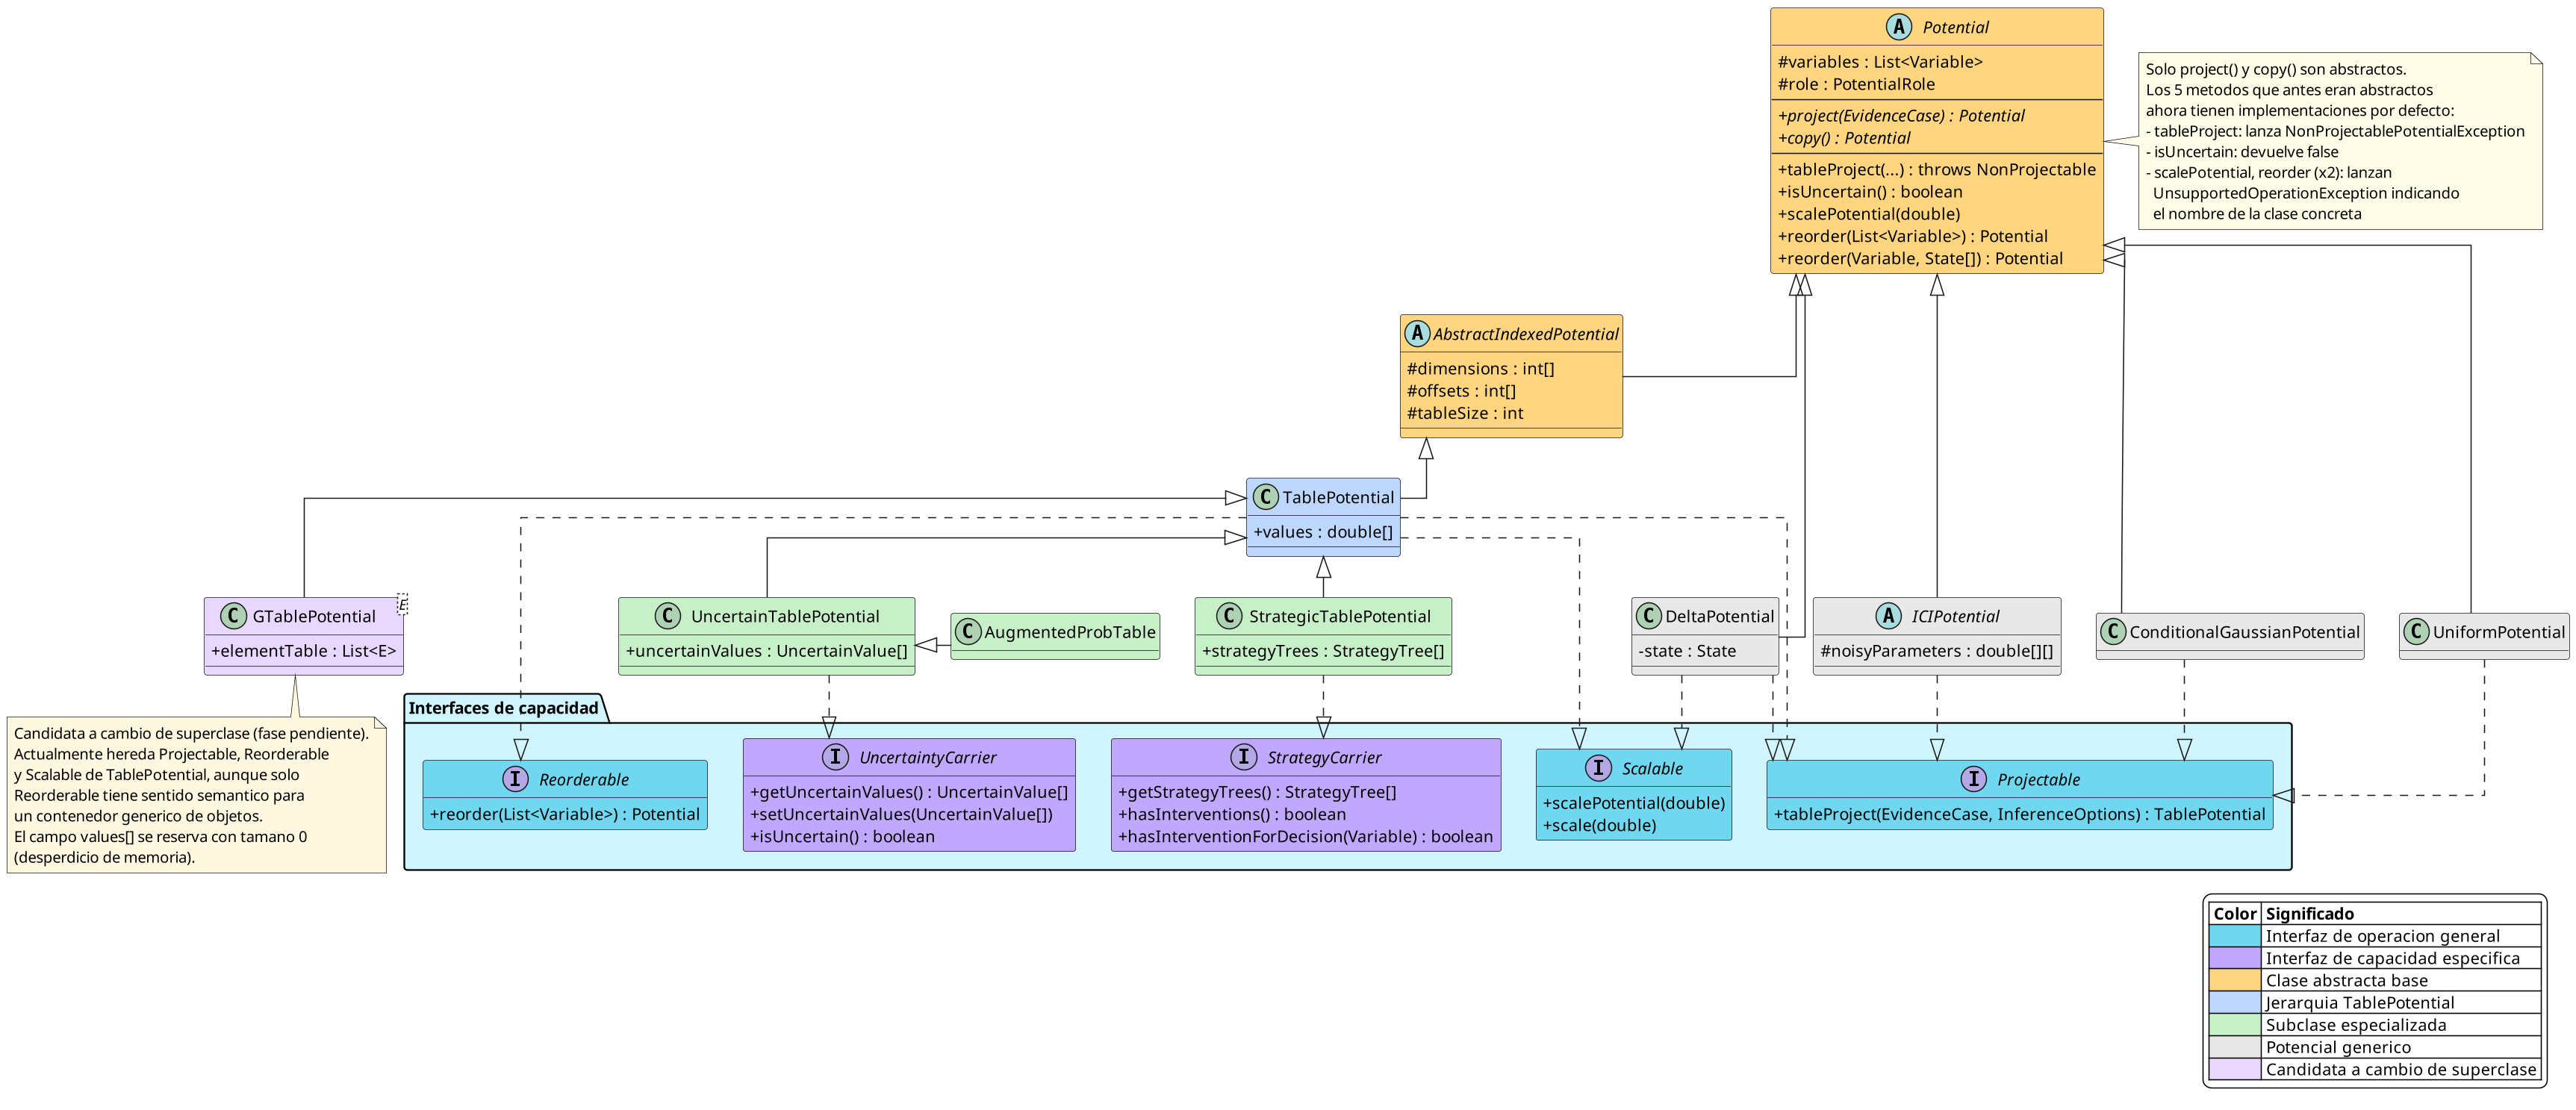
\includegraphics[width=\textwidth]{fig-op3-implementado.png}
\caption{Estado real de la jerarquía de potenciales tras completar los
         cuatro pasos del Rediseño~3.  Las interfaces de capacidad están
         operativas.  \code{Potential} ya no declara métodos abstractos
         innecesarios: solo \code{copy()} y \code{project(EvidenceCase)} son
         abstractos.  \code{GTablePotential} continúa extendiendo
         \code{TablePotential} (marcada en lila como candidata a
         cambio de superclase futura mediante la Opción~B descrita en la
         sección~\ref{sec:gtable-opcionB}).}
\label{fig:op3-implementado}
\end{figure}

% ===================================================================
\section{Divergencias respecto al diseño original}
\label{sec:impl-divergencias}

La implementación siguió el diseño en sus aspectos fundamentales, pero
se produjeron dos divergencias destacables.

\subsection{Nombre del método en \code{StrategyCarrier}}
\label{sec:impl-div-nombre}

El borrador del diseño nombraba el método \code{getStrategies()}.
La implementación final lo denominó \code{getStrategyTrees()}, en
coherencia con el nombre del campo subyacente (\code{strategyTrees[]}) y con
la terminología del dominio (los objetos son \emph{árboles de estrategia},
no estrategias abstractas).  El cambio es superficial y no afecta al diseño
estructural.

\subsection{Cambio de superclase de \code{GTablePotential}: aplazada}
\label{sec:impl-div-gtable}

El paso~4 del plan original incluía también cambiar la superclase
\code{GTablePotential} de \code{TablePotential} a
\code{AbstractIndexedPotential}.  Esta cambio de superclase se aplazó porque
la cadena de tipos en el módulo de coste-efectividad presenta bloqueadores
de compilación que requieren un diseño adicional.
La sección~\ref{sec:gtable-cambio de superclase} analiza este problema en detalle
y propone la solución a adoptar.

% ===================================================================
\section{Resultados de los tests}
\label{sec:impl-tests}

\begin{table}[H]
\centering
\begin{tabular}{l|rrr}
\toprule
\textbf{Módulo / Paso} & \textbf{Ejecutados} & \textbf{Fallos} & \textbf{Ignorados} \\
\midrule
\code{org.openmarkov.core} (Paso~1)              & 513 & 0 & 10 \\
\code{org.openmarkov.inference} (Paso~2)         &  13 & 0 &  3 \\
\code{org.openmarkov.integrationtests} (Paso~3)  & 368 & 0 & 51 \\
\code{org.openmarkov.integrationtests} (Paso~4)  & 368 & 0 & 51 \\
\bottomrule
\end{tabular}
\caption{Resultados de la batería de tests tras cada paso del Rediseño~3.
         Ningún paso introdujo regresiones.  Un test de GUI
         (\code{BasicOpenMarkovAppTest.testChangeNodeName}) presentó un fallo
         esporádico en la primera ejecución del Paso~3 pero pasó en
         ejecución aislada y en la segunda ejecución completa; se
         confirmó que es un problema preexistente de aislamiento de estado
         en tests de GUI, no relacionado con el Rediseño~3.}
\label{tab:impl-tests}
\end{table}

% ===================================================================
\section{Cambio de superclase de \code{GTablePotential}: análisis y decisión}
\label{sec:gtable-cambio de superclase}

\subsection{Motivación: por qué cambiar la superclase}
\label{sec:gtable-motiv}

\code{GTablePotential<E>} es un contenedor genérico de elementos indexados
por combinaciones de estados de variables.  Su campo central es
\code{List<E> elementTable}, donde \code{E} puede ser un \code{StrategyTree}
(en el análisis de coste-efectividad), una distribución de probabilidad,
u otro objeto de dominio.

Actualmente extiende \code{TablePotential}, que gestiona un array
\code{double[]~values}.  Esta relación de herencia es una \emph{herencia de
conveniencia}, no de \emph{es-un}: una \code{GTablePotential} no es una
\code{TablePotential} en el sentido semántico, sino que reutiliza la
mecánica de indexación (\code{dimensions[]}, \code{offsets[]},
\code{getConfiguration()}) que está implementada en
\code{AbstractIndexedPotential}.

Las consecuencias negativas de mantener la herencia actual son:

\begin{itemize}
  \item \textbf{Capacidades heredadas sin sentido}: \code{GTablePotential}
        hereda \code{Projectable} y \code{Scalable} de \code{TablePotential},
        aunque ninguna de las dos operaciones tiene sentido para un contenedor
        genérico de objetos.  Si el código llama
        \code{scalePotential(0.9)} sobre una \code{GTablePotential},
        ahora lanzará \code{UnsupportedOperationException} porque la
        implementación por defecto en \code{Potential} lo hace, pero
        la clase aparece en la tabla de interfaces como capaz de escalar
        (hereda \code{Scalable}), lo cual es engañoso.

  \item \textbf{Desperdicio de memoria}: el constructor de
        \code{GTablePotential} llama a \code{super(variables, null)}, que
        reserva \code{values = new double[tableSize]} con
        \code{tableSize} calculado a partir de las dimensiones ---aunque
        \code{values} jamas se use---.

  \item \textbf{Confusión para el lector del código}: cualquier método
        que recibe \code{TablePotential} puede recibir inadvertidamente una
        \code{GTablePotential} con \code{values.length > 0} (todos ceros)
        y \code{elementTable} no nulo, lo que puede producir cálculos
        numéricamente incorrectos sin lanzar ninguna excepción.
\end{itemize}

La cambio de superclase de \code{GTablePotential} a \code{AbstractIndexedPotential}
eliminaría estas anomalías y haría explícita la intención del
diseño: un contenedor genérico indexado que no es un potencial numérico.

\subsection{Bloqueadores del cambio de superclase}
\label{sec:gtable-bloqueadores}

La relación de herencia \code{GTablePotential extends TablePotential} está
explotada en tres lugares de la cadena de tipos del análisis de
coste-efectividad.

\subsubsection{Bloqueador~B1: Tipo de retorno de \code{DANInference.getUtility()}}

\begin{lstlisting}[caption={Campo y método afectados en \code{DANInference}}]
// DANInference.java  (modulo costEffectiveness)
private TablePotential utility;         // se asigna como GTablePotential<CEP>

public TablePotential getUtility() {
    return utility;
}
\end{lstlisting}

La variable \code{utility} se instancia como \code{GTablePotential<CEP>} pero
se declara como \code{TablePotential}.  Si \code{GTablePotential} dejara de
extender \code{TablePotential}, la asignación
\code{this.utility = new GTablePotential<>(...)} ya no compilaría.

\subsubsection{Bloqueador~B2: Cast en \code{DANCEAnalysis}}

\begin{lstlisting}[caption={Cast a \code{GTablePotential} en \code{DANCEAnalysis}}]
// DANCEAnalysis.java
GTablePotential<CEP> utility =
    (GTablePotential<CEP>) inferenceProcess.getUtility();
\end{lstlisting}

Si el tipo de retorno de \code{getUtility()} cambiara a \code{Potential},
el compilador rechazaría el cast como ``inconvertible types'': no existe
ninguna relación de tipo entre \code{Potential} y \code{GTablePotential}
que garantice que el cast es correcto en tiempo de compilación.

\subsubsection{Bloqueador~B3: Listas \code{List<TablePotential>} en \code{TablePotentialMerge}}

\begin{lstlisting}[caption={Parámetro de tipo en \code{TablePotentialMerge} y \code{CEDecisionTreeNode}}]
// TablePotentialMerge.java
public static TablePotential merge(List<TablePotential> potentials) { ... }

// CEDecisionTreeNode.java
public void setOnlyValueForUtility(TablePotential utility) {
    // ... cast interno a (GTablePotential) ...
}
\end{lstlisting}

En el flujo CE, estos métodos reciben listas o parámetros que contienen
instancias de \code{GTablePotential}.  Si \code{GTablePotential} deja de
extender \code{TablePotential}, los sitios de llamada dejan de compilar.

La figura~\ref{fig:gtable-cadena-ce} ilustra estas dependencias de tipo y
los tres bloqueadores.

\begin{figure}[H]
\centering
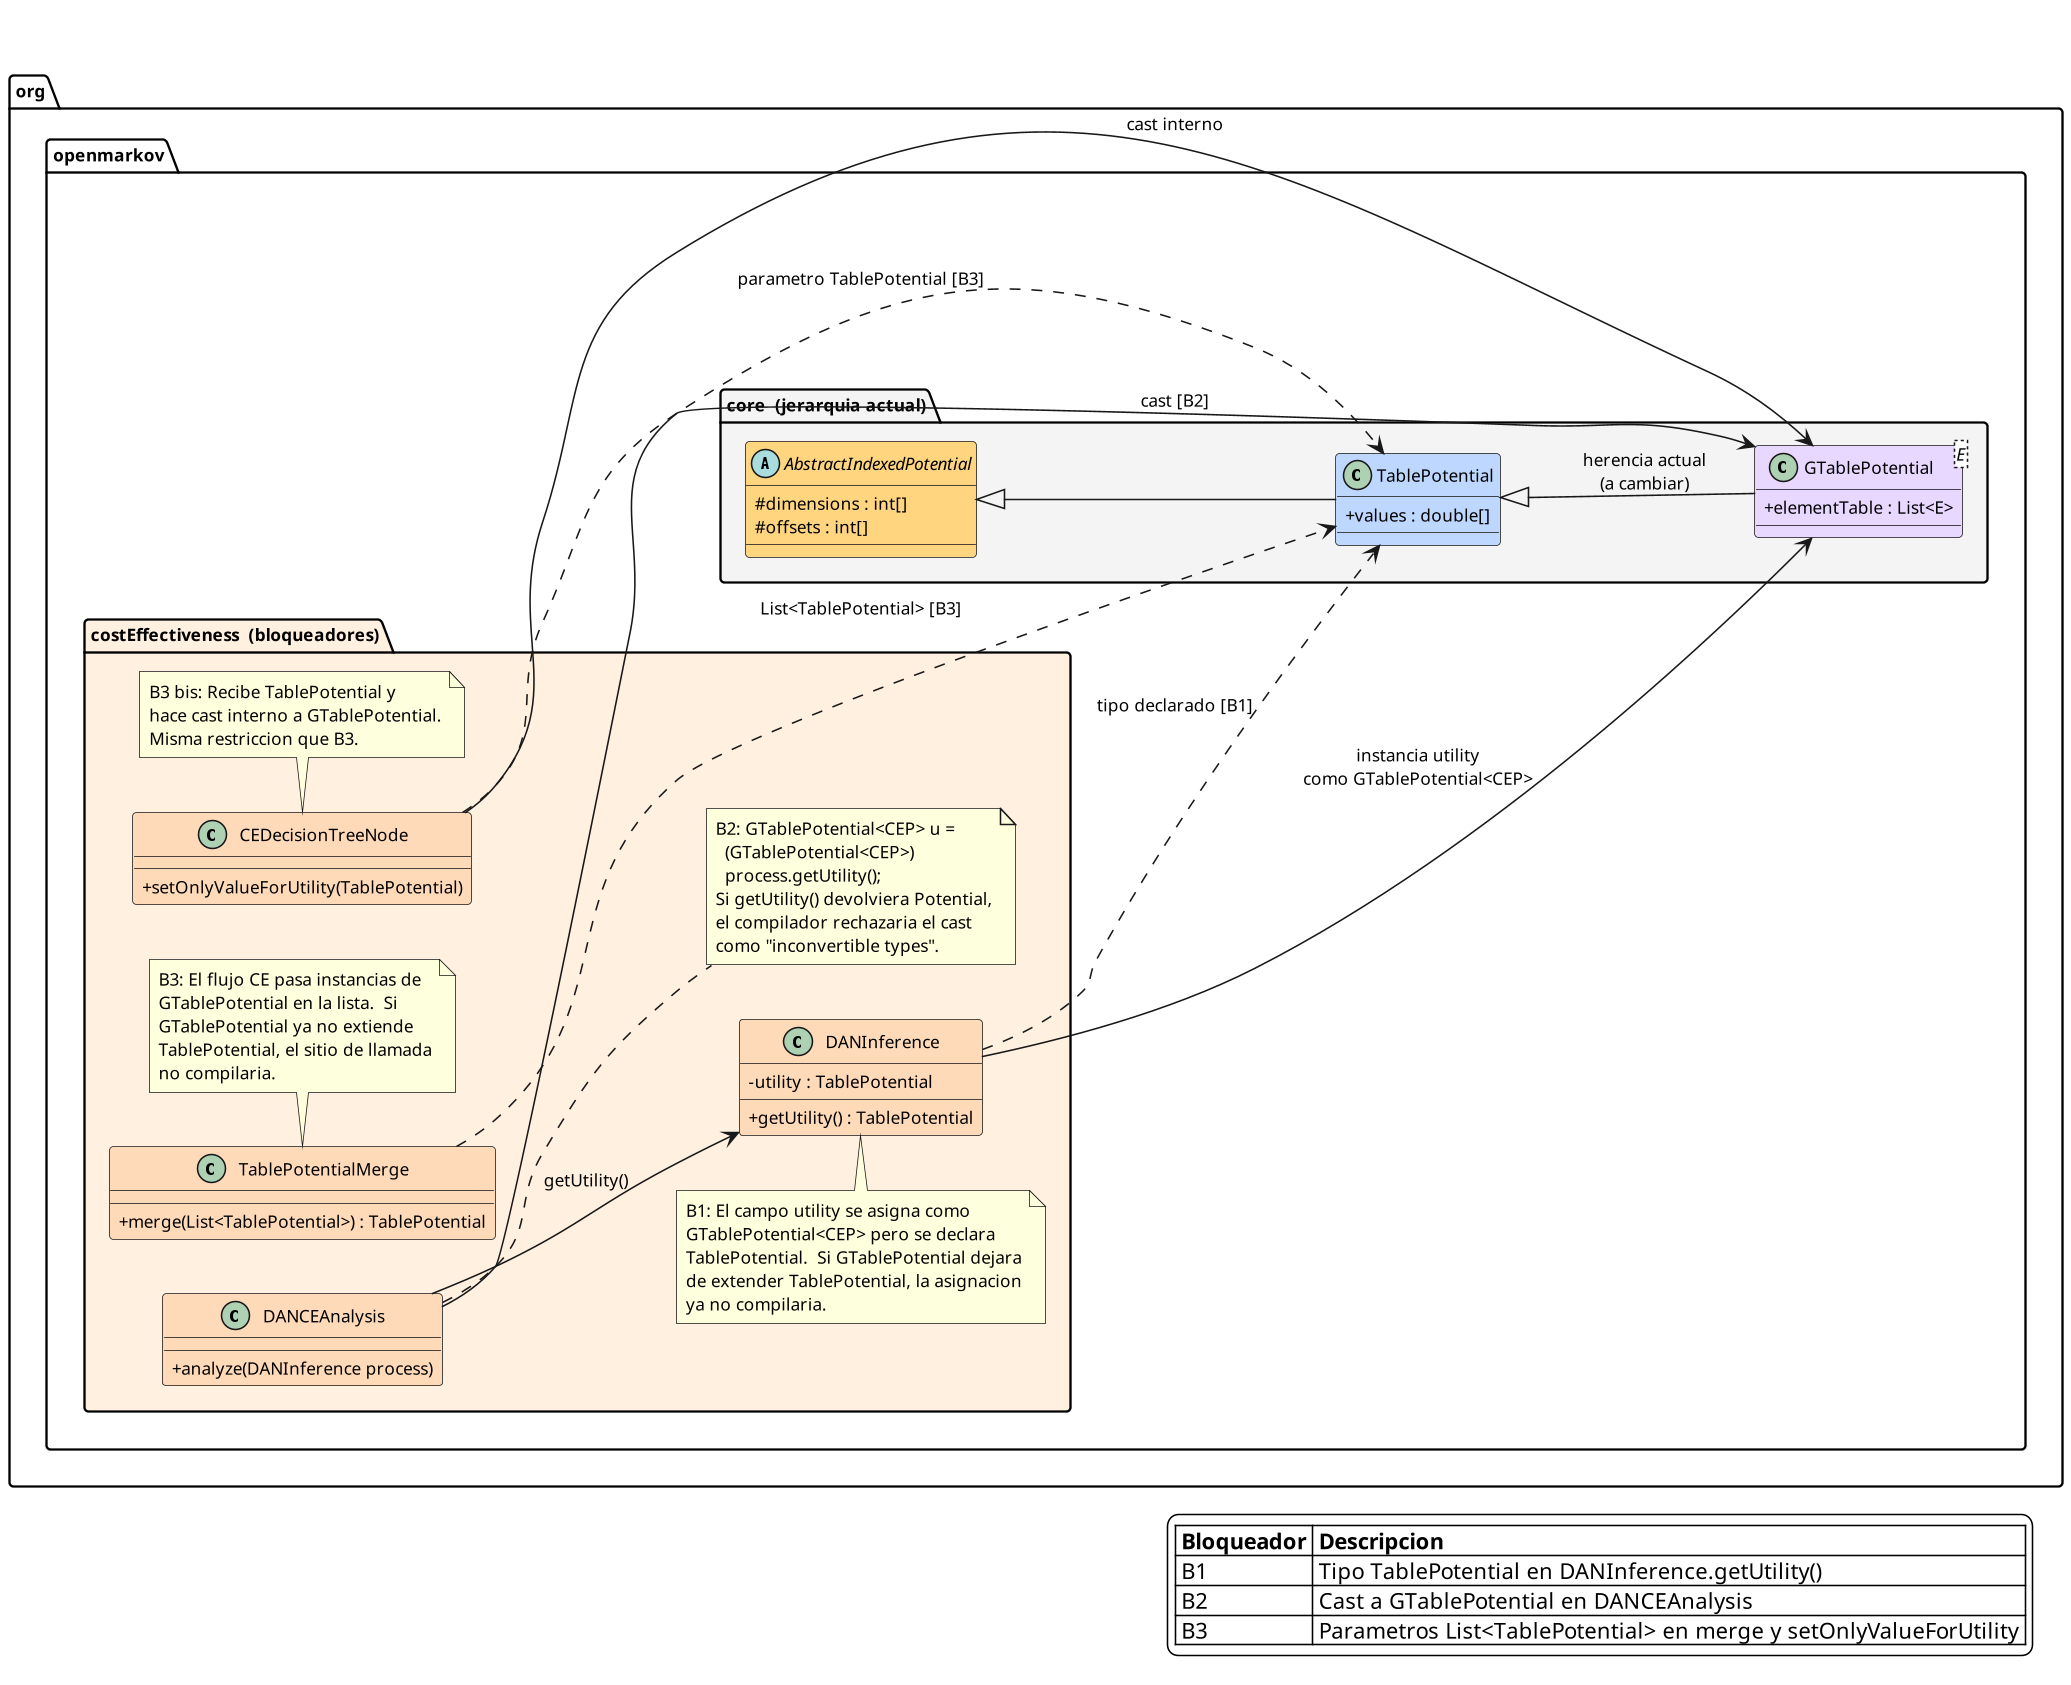
\includegraphics[width=\textwidth]{fig-gtable-cadena-ce.png}
\caption{Cadena de tipos en el análisis de coste-efectividad que bloquea la
         cambio de superclase de \code{GTablePotential}.  Los tres bloqueadores
         B1, B2 y B3 aparecen en clases distintas del módulo
         \code{costEffectiveness}.}
\label{fig:gtable-cadena-ce}
\end{figure}

\subsection{Opción~A: generalizar los tipos a \code{Potential}}
\label{sec:gtable-opcionA}

La Opción~A resuelve los bloqueadores cambiando los tipos declarados en
la cadena CE para que usen \code{Potential} en lugar de \code{TablePotential}:

\begin{lstlisting}[caption={Cambios en la Opción~A: generalizar a \code{Potential}}]
// DANInference.java
private Potential utility;                // antes: TablePotential
public Potential getUtility() { ... }     // antes: TablePotential

// DANCEAnalysis.java  (sin cambio, el cast sigue siendo valido)
GTablePotential<CEP> u = (GTablePotential<CEP>) process.getUtility();

// TablePotentialMerge.java
public static Potential merge(List<Potential> potentials) { ... }
                                          // antes: List<TablePotential>
\end{lstlisting}

Esta opción requiere muy pocos cambios de código, pero tiene implicaciones
de diseño problemáticas:

\begin{itemize}
  \item \textbf{Pérdida de tipo explícito en la API}: \code{getUtility()}
        devolvía un tipo que garantizaba la posibilidad de hacer operaciones
        numéricas sobre valores dobles.  Con \code{Potential}, el código
        cliente debe confiar implícitamente en que \emph{de hecho} recibe
        algo numéricamente manejable, o bien hacer más casts.

  \item \textbf{Regresión potencial en \code{TablePotentialMerge}}: al
        aceptar \code{List<Potential>}, el método puede recibir cualquier
        tipo de potencial ---incluyendo \code{UniformPotential} o
        \code{DeltaPotential}--- para los que el algoritmo de \emph{merge}
        no está definido.  El error solo se manifestaría en tiempo de
        ejecución.

  \item \textbf{Inconsistencia con los objetivos del Rediseño~3}: el
        objetivo central era hacer los tipos más precisos, no generalizarlos.
        La Opción~A iría en dirección contraria en estos puntos de la API.
\end{itemize}

\subsection{Opción~B: nueva interfaz \code{CEUtilityPotential}}
\label{sec:gtable-opcionB}

La Opción~B introduce una nueva interfaz de dominio ---\code{CEUtilityPotential}---
que captura el contrato común entre \code{TablePotential} y
\code{GTablePotential} en el contexto del análisis de coste-efectividad.
Ambas clases implementan esta interfaz; la cadena CE la usa como tipo de
referencia en lugar de \code{TablePotential}:

\begin{lstlisting}[caption={Nueva interfaz \code{CEUtilityPotential} (Opción~B)}]
/**
 * Marca un potencial que puede actuar como utilidad en el analisis
 * de coste-efectividad de DANs.  Implementada por TablePotential
 * y GTablePotential<E>.  Actua como lista blanca de tipos validos
 * en la cadena CE, previniendo que tipos inadecuados lleguen a los
 * algoritmos de fusion (TablePotentialMerge) o de arbol (CEDecisionTreeNode).
 */
public interface CEUtilityPotential {
    // Interfaz marcadora; puede ampliarse con metodos compartidos
    // (getDimensions(), getOffsets()) si se necesita acceso indexado
    // sin cast posterior.
}
\end{lstlisting}

\begin{lstlisting}[caption={Cambios necesarios en el módulo \code{core} (Opción~B)}]
// GTablePotential: superclase cambiada a AbstractIndexedPotential
public class GTablePotential<E> extends AbstractIndexedPotential
        implements Reorderable, CEUtilityPotential { ... }
    // Ya no hereda Projectable ni Scalable de TablePotential

// TablePotential: anade CEUtilityPotential a sus interfaces existentes
public class TablePotential extends AbstractIndexedPotential
        implements Projectable, Reorderable, Scalable, CEUtilityPotential { ... }
\end{lstlisting}

\begin{lstlisting}[caption={Cambios en la cadena CE (Opción~B)}]
// DANInference.java  -- B1 resuelto
private CEUtilityPotential utility;
public CEUtilityPotential getUtility() { return utility; }

// DANCEAnalysis.java  -- B2 resuelto
// El cast es valido porque GTablePotential implementa CEUtilityPotential
GTablePotential<CEP> u = (GTablePotential<CEP>) process.getUtility();

// TablePotentialMerge.java  -- B3 resuelto
public static CEUtilityPotential merge(
        List<CEUtilityPotential> potentials) { ... }
\end{lstlisting}

La figura~\ref{fig:gtable-opcionB} muestra el diseño completo de la
Opción~B.

\begin{figure}[H]
\centering
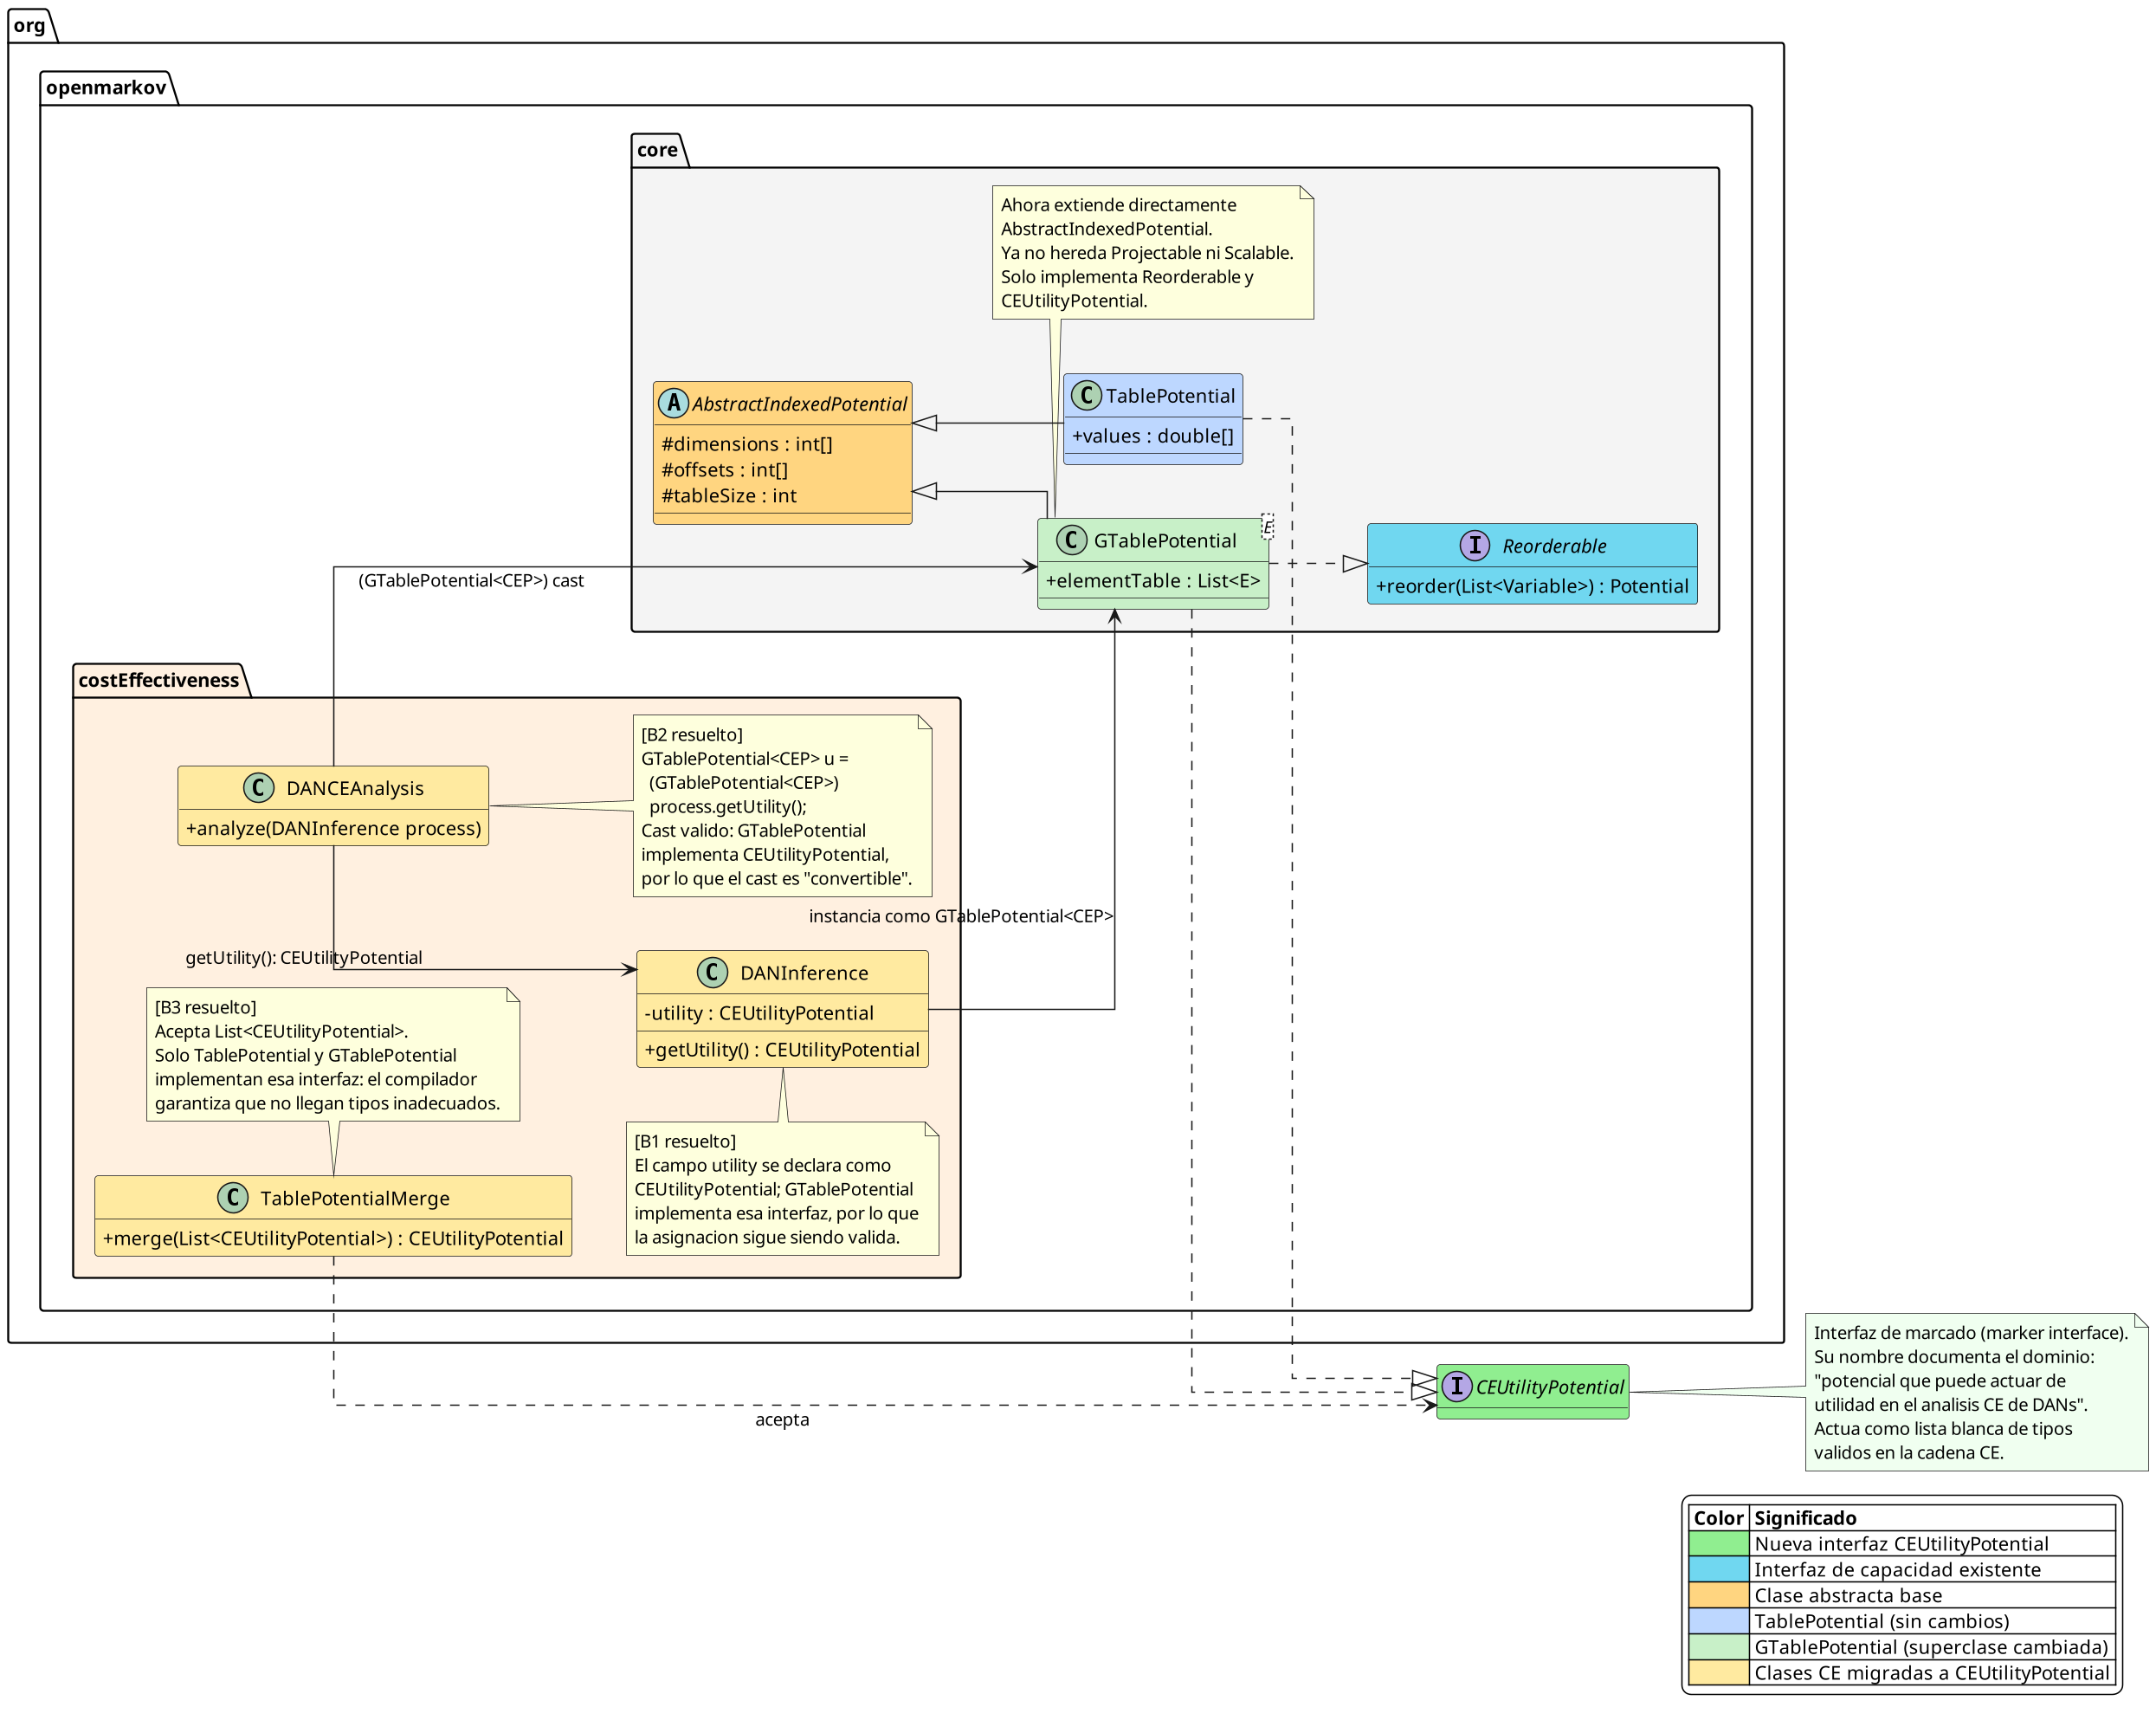
\includegraphics[width=0.9\textwidth]{fig-gtable-opcionB.png}
\caption{Opción~B: la interfaz \code{CEUtilityPotential} permite cambiar la superclase
         \code{GTablePotential} a \code{AbstractIndexedPotential} sin perder
         tipo en la cadena CE.  \code{TablePotential} y \code{GTablePotential}
         implementan la nueva interfaz; los tres bloqueadores B1, B2, B3
         quedan resueltos con cambios localizados.}
\label{fig:gtable-opcionB}
\end{figure}

\subsection{Comparación entre opciones}
\label{sec:gtable-comparacion}

\begin{table}[H]
\centering
\small
\setlength{\tabcolsep}{4pt}
\begin{tabular}{p{3.0cm}|p{4.8cm}|p{4.8cm}}
\toprule
\textbf{Criterio}
  & \textbf{Opción~A (generalizar a \code{Potential})}
  & \textbf{Opción~B (nueva interfaz \code{CEUtilityPotential})} \\
\midrule
\textbf{Mantenibilidad} &
  Baja: \code{getUtility()} devuelve \code{Potential}, lo que obliga a
  futuros desarrolladores a conocer implícitamente que el objeto
  es en realidad un \code{GTablePotential} &
  Alta: la interfaz \code{CEUtilityPotential} documenta explícitamente
  qué tipos son válidos en la cadena CE \\
\midrule
\textbf{Inteligibilidad} &
  Baja: usar \code{Potential} donde la semántica requiere un objeto
  indexado genera confusión; el contrato implícito no es visible en
  la firma &
  Alta: la interfaz es autodocumentada; su nombre expresa tanto el
  dominio (\emph{coste-efectividad}) como el rol (\emph{utilidad}) \\
\midrule
\textbf{Elegancia} &
  Media: pocos cambios, pero el resultado es una API más laxa que
  la original, contradiciendo los objetivos del Rediseño~3 &
  Alta: coherente con el patrón de interfaces de capacidad ya
  introducido; un nuevo tipo de dominio, no una generalización
  hacia \emph{cualquier} potencial \\
\midrule
\textbf{Riesgo de regresión} &
  Alto: \code{TablePotentialMerge} con \code{List<Potential>} puede
  recibir tipos inesperados y fallar en tiempo de ejecución sin
  error de compilación &
  Bajo: solo \code{TablePotential} y \code{GTablePotential} implementan
  \code{CEUtilityPotential}; el compilador garantiza que no llegan tipos
  inadecuados \\
\midrule
\textbf{Volumen de cambios} &
  Muy bajo: 3--4 líneas modificadas &
  Bajo: 1 fichero nuevo de interfaz + 4--5 líneas modificadas \\
\bottomrule
\end{tabular}
\caption{Comparación entre la Opción~A (generalizar tipos a \code{Potential})
         y la Opción~B (nueva interfaz \code{CEUtilityPotential}) para
         resolver los bloqueadores de la cambio de superclase de \code{GTablePotential}.}
\label{tab:gtable-comparacion}
\end{table}

\subsection{Decisión: Opción~B}
\label{sec:gtable-decision}

Se adopta la \textbf{Opción~B} por las siguientes razones:

\begin{enumerate}
  \item \textbf{Coherencia con el Rediseño~3}: el patrón de interfaces
        de capacidad ya estabilizado hace natural introducir una interfaz de
        dominio específico (\code{CEUtilityPotential}) en lugar de
        generalizar a \code{Potential}.  Añadir una interfaz es
        exactamente el tipo de cambio que el Rediseño~3 promueve.

  \item \textbf{Seguridad de tipos en tiempo de compilación}: la interfaz
        actúa como una \emph{lista blanca} de tipos válidos para la cadena
        CE.  Ninguna subclase de \code{Potential} puede introducirse
        accidentalmente en \code{TablePotentialMerge} sin declarar
        explícitamente que implementa \code{CEUtilityPotential}.

  \item \textbf{Bajo riesgo de regresión}: los cambios se concentran en
        \code{DANInference}, \code{DANCEAnalysis},
        \code{TablePotentialMerge} y \code{CEDecisionTreeNode}.
        El algoritmo de cálculo no cambia; solo cambian los tipos declarados
        de las variables.

  \item \textbf{Documentación implícita}: el nombre
        \code{CEUtilityPotential} comunica en el código fuente
        el dominio de uso y el rol del objeto, facilitando la comprensión
        a futuros desarrolladores sin necesidad de consultar documentación
        externa.
\end{enumerate}

La implementación de la Opción~B se planifica como \textbf{Fase~5 del
Rediseño~3}, una vez que los cuatro pasos ya ejecutados hayan sido
validados en un ciclo de integración completo.

% ===================================================================
\section{Encapsulación del campo \code{values} en \code{TablePotential}}
\label{sec:encapsulacion-values}

% -------------------------------------------------------------------
\subsection{Situación anterior}

El campo que almacena la tabla numérica de un potencial discreto era
\textbf{público y volátil}:

\begin{lstlisting}[caption={Campo \texttt{values} antes de la encapsulación.},
                   label=lst:values-antes]
/**
 * Table storing the numerical values of the potential. This attribute is
 * public for efficiency and volatile for efficiency in concurrent operations.
 */
public volatile double[] values;
\end{lstlisting}

El campo \code{values} era accedido directamente en \textbf{135~puntos}
del proyecto, en módulos tan variados como \code{inference},
\code{gui}, \code{io} y \code{learning}.  El comentario del código
original justificaba la visibilidad pública con un argumento de
rendimiento, y la palabra clave \code{volatile} con un argumento de
seguridad en entornos concurrentes.

% -------------------------------------------------------------------
\subsection{Problemas del diseño anterior}

\paragraph{El campo público viola la encapsulación (antipatrón
\emph{Aliasing Bug}).}

Un campo de array público mutable es una fuente clásica de
\emph{aliasing bugs} (§\ref{sec:fund-alias-bug}).  Cualquier fragmento
de código que escriba \code{pot.values} obtiene una referencia
directa al array interno.  Si ese código almacena la referencia en
una variable local y después modifica el array a través de esa
variable, la modificación se refleja silenciosamente en el potencial
original, sin que la clase pueda detectarlo ni impedirlo.

En OpenMarkov este riesgo era real: los algoritmos de inferencia copian
potenciales, los transforman y los almacenan.  Si en algún momento
dos variables apuntaban al mismo array, una operación sobre una de
ellas modificaba el estado del otro potencial.

\paragraph{\code{volatile} no protege los contenidos del array.}

La palabra clave \code{volatile} en Java garantiza que \textbf{la
referencia} al array se lee y escribe de forma atómica y que los
cambios son visibles entre hilos~\cite{goetz2006}.  Sin embargo,
\code{volatile} no protege los \emph{contenidos} del array: dos hilos
pueden leer la misma referencia y acceder a posiciones distintas del
array sin ninguna exclusión mutua.

El comentario del código original afirmaba que \code{volatile} era
necesario para la concurrencia, pero eso era incorrecto: la
declaración creaba una \textbf{falsa sensación de seguridad}.  El
array podría corromperse concurrentemente aunque la referencia fuera
volátil.  La anotación correcta habría requerido un
\code{AtomicReferenceArray} o bien sincronización explícita, ninguna
de las cuales era práctica dado el uso del campo.

\paragraph{La visibilidad pública impide cambiar la representación.}

Mientras el campo sea público, cualquier cambio en el tipo o la
estructura interna de la tabla (por ejemplo, almacenarla como
\code{float[]} en lugar de \code{double[]} para reducir memoria, o
como una lista dispersa para potenciales con muchos ceros) obligaría
a modificar los 135~sitios que acceden directamente al campo.  Con un
campo privado y un par de métodos, ese cambio sería transparente para
todos los llamadores.

% -------------------------------------------------------------------
\subsection{La encapsulación: \code{private} + \code{getValues()} + \code{setValues()}}

El cambio consiste en hacer el campo privado y canalizar todo acceso
a través de dos métodos:

\begin{lstlisting}[caption={Campo \texttt{values} después de la encapsulación.},
                   label=lst:values-despues]
/**
 * Table storing the numerical values of the potential.
 * Use getValues() for read access and setValues(double[]) for bulk assignment.
 */
private double[] values;

/**
 * Returns the internal values array directly (live reference, not a copy).
 * Callers must not assign a new array to the returned reference; use
 * setValues(double[]) for bulk replacement.
 */
public double[] getValues() {
    return values;
}

/**
 * Replaces the values array.
 *
 * @param newValues new values array
 */
public void setValues(double[] newValues) {
    this.values = newValues;
}
\end{lstlisting}

Nótese que \code{getValues()} devuelve la referencia interna, no una
copia.  Esto es deliberado: copiar el array en cada acceso sería
prohibitivo para los algoritmos de inferencia, que leen y escriben el
array en bucles internos.  El Javadoc advierte explícitamente de que
el llamador no debe reasignar la referencia devuelta.  Lo que se gana
no es inmutabilidad completa, sino \textbf{encapsulación del punto de
sustitución}: si alguien quiere reemplazar el array por otro, debe
llamar a \code{setValues()}, que es el único lugar donde se puede
añadir lógica futura (auditoría, invalidación de cachés, etc.).

% -------------------------------------------------------------------
\subsection{Por qué \texttt{setValues()} no valida el tamaño}
\label{sec:setvalues-sin-validacion}

La primera versión de \code{setValues()} incluía una comprobación de
tamaño aparentemente razonable:

\begin{lstlisting}[caption={Validación de tamaño que se consideró y se descartó.},
                   label=lst:setvalues-validacion]
// Version descartada -- rompe SystematicSampling
public void setValues(double[] newValues) {
    if (newValues.length != tableSize) {
        throw new IllegalArgumentException(
            "Expected " + tableSize + " values, got " + newValues.length);
    }
    this.values = newValues;
}
\end{lstlisting}

Añadir esa validación parece una buena práctica de programación
defensiva: si alguien intenta asignar un array de tamaño incorrecto,
el error se detecta inmediatamente en lugar de producir resultados
silenciosamente erróneos.

Sin embargo, la validación rompía el módulo de análisis de
sensibilidad (\code{SystematicSampling}).  Ese algoritmo realiza
múltiples ejecuciones de inferencia variando un parámetro y almacena
los resultados de todas las muestras en un \textbf{único array
sobredimensionado}: si el potencial tiene \code{tableSize}~$= n$ y
hay $k$~muestras, el array almacenado tiene longitud $k \cdot n$.  El
array sobredimensionado es la estructura interna elegida para evitar
la creación de $k$~potenciales distintos.  Es un uso deliberado y
válido, pero viola el supuesto invariante \code{values.length ==
tableSize}.

Esta situación ilustra una lección importante de diseño: \textbf{no
añadir validación para supuestos invariantes que no son invariantes
universales}.  El contrato de \code{setValues()} es simplemente
``reemplaza el array interno''; no establece ninguna relación entre el
tamaño del nuevo array y \code{tableSize}.  Añadir esa restricción
sería sobredefinir el contrato en perjuicio de usos legítimos.

La validación correcta, si se desea, debe hacerse en los lugares
donde sí se conoce el contrato preciso ---por ejemplo, en los
constructores que inicializan el array con \code{tableSize} posiciones,
o en los algoritmos que dependen de la alineación entre \code{values}
y \code{tableSize}--- y no en el método de acceso genérico.

% -------------------------------------------------------------------
\subsection{Migración y efectos secundarios}

La migración de los 135~accesos directos al campo fue realizada con un
script automatizado que sustituyó \code{pot.values} por
\code{pot.getValues()} y \code{pot.values = x} por
\code{pot.setValues(x)}.

El script introdujo inadvertidamente un error en la clase
\code{Choice}: su propio método \code{setValues(int[])} contenía la
asignación \code{this.values = values} (sobre el campo \code{int[]
values} de \code{Choice}, no sobre \code{TablePotential}).  El script
transformó esa línea en \code{this.setValues(values)}, generando una
\textbf{recursión infinita} que terminaba en \code{StackOverflowError}.
El error se detectó al ejecutar los tests y se corrigió restaurando la
asignación directa al campo:

\begin{lstlisting}[caption={Corrección de la recursión infinita en \texttt{Choice.setValues()}.},
                   label=lst:choice-setvalues]
// Antes (error introducido por el script de migracion):
public void setValues(int[] values) {
    this.setValues(values);  // llamada recursiva infinita
    numValues = values.length;
    initialized = true;
}

// Despues (corregido):
public void setValues(int[] values) {
    this.values = values;    // asignacion directa al campo propio de Choice
    numValues = values.length;
    initialized = true;
}
\end{lstlisting}

Este incidente es un ejemplo de por qué las migraciones automatizadas
a gran escala deben ir acompañadas de una suite de tests completa: el
error se manifestó como un fallo de test inmediato y claro
(\code{StackOverflowError}), lo que permitió localizarlo y corregirlo
sin dificultad.

% -------------------------------------------------------------------
\subsection{Resultado}

\begin{center}
\begin{tabular}{lll}
\toprule
\textbf{Aspecto} & \textbf{Antes} & \textbf{Después} \\
\midrule
Visibilidad del campo   & \code{public volatile} & \code{private} \\
Acceso de lectura       & directo (\code{pot.values})   & \code{pot.getValues()} \\
Acceso de escritura     & directo (\code{pot.values = x}) & \code{pot.setValues(x)} \\
Protección concurrente  & \bad{falsa} (\code{volatile} solo protege la referencia) & sin cambio (pendiente) \\
Sitios de acceso directo & 135 & 0 \\
Validación de tamaño    & ninguna & ninguna (deliberado: \code{SystematicSampling}) \\
Bugs introducidos       & --- & \warn{1} (\code{Choice}, corregido en el mismo commit) \\
\bottomrule
\end{tabular}
\end{center}

La encapsulación no resuelve el problema de seguridad en entornos
concurrentes ---eso requeriría una refactorización más profunda--- pero
sí elimina el riesgo de \emph{aliasing bugs} a través de asignaciones
directas al campo y abre la puerta a añadir lógica en el único punto
de acceso en el futuro.  Es el primer paso de la cadena
encapsulación~$\to$ abstracción~$\to$ sustitución de representación,
sin comprometer la compatibilidad con el código existente.

\begin{thebibliography}{9}
\bibitem{martin2003}
  Robert C. Martin,
  \emph{Agile Software Development: Principles, Patterns, and Practices},
  Prentice Hall, 2003.

\bibitem{liskov1994}
  Barbara H. Liskov y Jeannette M. Wing,
  ``A Behavioral Notion of Subtyping'',
  \emph{ACM Transactions on Programming Languages and Systems},
  vol.~16, n.~6, pp.~1811--1841, noviembre de 1994.

\bibitem{gamma1995}
  Erich Gamma, Richard Helm, Ralph Johnson y John Vlissides,
  \emph{Design Patterns: Elements of Reusable Object-Oriented Software},
  Addison-Wesley, 1995.

\bibitem{goetz2006}
  Brian Goetz, Tim Peierls, Joshua Bloch, Joseph Bowbeer, David Holmes y
  Doug Lea,
  \emph{Java Concurrency in Practice},
  Addison-Wesley, 2006.
\end{thebibliography}

\end{document}
